%//////////////////////////////////////////////////////////////////////
% 2013年度 情報学群実験第3C・第4C テキスト
%                                       高知工科大学情報学群
%//////////////////////////////////////////////////////////////////////
\documentclass[10pt]{text2002}
\usepackage{eclbkbox}
\usepackage{alltt}
\usepackage{ascmac}
\usepackage[dvipdfm]{graphicx}
\usepackage{graphicx}
\usepackage{multicol}
\usepackage{fancybox}
\usepackage{jumoline}

\newcommand{\ttt}[1]{\texttt{#1}}

% \makeatletter
%      \def\sloppy{%
%        \tolerance 9999%
%        \emergencystretch 3em%
%        \hfuzz .5\p@
%        \vfuzz\hfuzz}
% \makeatother

%	enumerate 環境の変更
\renewcommand{\labelenumi}{(\theenumi)}

%	keybox(ascmac.sty の \keytop の中身をタイプライタ体に変更)
\def\keybox#1{{\keytop{\tt#1}}}

%	taskbar(文字列を囲む枠)
\def\taskbar#1{\setlength{\fboxrule}{0.5pt}\fbox{#1}}

%	Hline(tabular 環境内の \hline よりも太い横線)
%		from IEICE LaTeX Macro
\def\Hline{\noalign{\hrule height 0.4mm}}
%	enumerate 環境の変更
\renewcommand{\labelenumi}{(\theenumi)}

%	Gcenter(tabular 環境内の縦方向のセンタリング)
%		written by Otobe Yoshiki
\newcommand{\Gcenter}[2]{
    \dimen0 = \ht\strutbox
    \advance\dimen0\dp\strutbox
    \multiply\dimen0 by#1
    \divide\dimen0 by2
    \advance\dimen0 by-.5\normalbaselineskip
    \raisebox{-\dimen0}[0pt][0pt]{#2}}

  \makeatletter
    \newenvironment{cli}%
    {\VerbatimEnvironment
     \begin{center}
     \begin{breakbox}
     \begin{Verbatim}
        }%
    {%
     \end{Verbatim}
     \end{breakbox}
     \end{center}
     }
  \makeatother

  \makeatletter
    \newenvironment{cli-tex}%
    {\begin{center}
     \begin{breakbox}
     \begin{alltt}
        }%
    {%
     \end{alltt}
     \end{breakbox}
     \end{center}
     }
  \makeatother

\newif\ifTA
\TAfalse

\title{}
\author{}
\date{}

\begin{document}
\sloppy
\maketitle
%----------------------------------------------------------------------- 目次
\pagenumbering{roman}
%   目次はローマ数字
\chapter*{序~~論}\label{chapter:introduction}
%
%   はじめに
%        written by Shinichi Yoshida
%        April 13, 2018

昨今,人工知能(機械学習とビッグデータ処理)関連の技術の進展が目覚しく,
人間の行う職業がなくなりつつあるように見受けられる.例えば,自動運転技術
が進展することで,バスやトラック,タクシーなどの職業が衰退することも考え
られる.エンジニア職も例外ではない.ネットワークエンジニアは将来なくなる
職業にとりあげられることもある.しかしながら,人工知能技術は,明確なルー
ルがあるものや,単調な作業などはすぐに置き換えることができるが,複雑なも
のになればなるほど,機械学習アルゴリズムでは学習ができない.一方,ネット
ワーク技術が様々な技術の集合体であり,場所によって異なる形で構築がされる
ような複雑なシステムである.全ての機器が設計通りに動いているのならばまだ
しも,停電や経年劣化,障害等で一部の機器が動作停止や誤動作するようなこと
もある.こうした複雑かつ困難な状況に,即座に柔軟に対処できるような AI は
まだ見当たらない.このような観点から考えると,ますます複雑になるネットワー
クシステムを支える技術者は,今後しばらくは(少なくとも我々が職業を持って
働く間は)なくなることはないであろう.

さらに言えば,Facebook, Twitter, LINE などの SNS,Google, Dropbox,
Amazon, Microsoft 等の様々なサービスやクラウド技術など,インターネットサー
ビスが発展し,多くの人々が利用している.これらは,インターネットのインフ
ラが稼働していないと全く利用できない.すなわち,これらに障害が起きると生
活に支障が出るくらい,重要な生活のインフラストラクチャ(基盤)になってい
ると言え,これらを支えることは現代では電気・エネルギーや水道,運輸インフ
ラを支えると同じくらい重要なことである.

また,セキュリティも重要な事項であり,他のインフラと異なり,インターネッ
トインフラはサイバー攻撃による影響がとても大きく,一つの企業や国の生活に
影響を与えるほどである.実際に,通常の軍隊と同様に,サイバー軍を創設し他
国への攻撃,他国からの攻撃に備える国も増えている.さらには,先ほどの人工
知能も人々のインターネットの利用が進み,さらには IoT (Internet of
Things) などで多くの機器がインターネット接続され,多くのデータが蓄積され
たことで,はじめて人工知能が構築可能になったとも言える.

以上のことから,インターネット技術を実際に体験し習得することは,今後の情
報技術者にとって重要なことであるのは間違いない.この実験では,こうしたイ
ンターネット技術を支える技術について,実際に構築をしながら,幅広い角度か
らネットワーク技術を学ぶ.本実験で扱う技術は,必ずしも最新のサービスでは
なく,今後も長く使われ続ける基礎技術に重点を置いている.UNIX系OS(Ubuntu
Linux,CentOS), Windows, Macintosh といった広く普及しているオペレーティ
ングシステムを用いて,それぞれのコンピュータのネットワーク設定ならびに,
サーバでのWWWやデータベースシステム,暗号化など,身近に使われているネッ
トワークサービスの構築を行う.さらに,ルーティング,ネットワーク設計,ス
イッチ設定,VLAN,セキュリティといったインターネットを支える基盤技術の構
築を,ネットワーク業界で広く使われる Cisco IOS を実際に用いて学ぶ.IOS 
は CCNA 試験など,ネットワーク業界で認められている資格試験にも使われてお
り,多くのベンダが IOS 互換のコマンド体系を採用していることからネットワー
クを学ぶのに最も適したシステムといっても良い.

本実験の内容は初学の者にとっては十分に複雑で難しいものであるかも知れな
い.しかし,本実験の内容はまだまだ基礎であり,この先にはさらに複雑で設
計の難易度の高いシステムが数多く存在している.ぜひ,この実験を通して基
礎技術,基盤技術を身に付け,将来,更なる発展技術の習得,および新技術,
新サービスの開発へと進んでいき,インターネットの発展に寄与して欲しいと
考える.

全ての専攻の学生が,このテキストと実験での経験をもとに,ネットワーク技術
の仕組みを理解し,様々な業界で活躍することを心より期待し,巻頭の言とする.

\begin{flushright}
 2019年4月13日

 情報学群実験3i・4C 教育担当スタッフ一同
\end{flushright}

\clearpage
\chapter*{レポートについて}\label{chapter:report}


レポートは,下記の体裁にて提出すること.\textbf{全てのレポートについて,
1つでも下記に該当する場合,採点および単位認定されない} ので注意すること.

\begin{itemize}
 \item \textbf{指定された期日・時刻までに提出されない場合}
 \item \textbf{指定された様式でない場合,特に抜けている項目がある場合}
\end{itemize}

加えて,\textbf{下記の場合は,単位認定されない上に,不正行為として処罰さ
れる行為}であるので,厳に慎むこと.

\begin{itemize}
 \item \textbf{他人のレポートからの転載}
 \item \textbf{他の Web ページ,本などからの転載}
\end{itemize}

本科目のレポートは,全て,KUT LMS (Learning Management System,
https://lms.kochi-tech.ac.jp )の本科目の項目から PDF にて提出する.提出
されたレポートは,\textbf{Turnitin システムにより,過去も含む他人のレポー
ト,Webページ,出版された本などと一致する文章があるか照合され,剽窃チェッ
クが行われる.}

LaTeX (platex) にて,実験の冒頭で指定されたテンプレートを用いて作成する
こと.

\textbf{章立ては下記の通りとすること.下記の項目に従っていないもの,一部の項目に
抜けがある不完全なものは,提出されても受理しない.}

\begin{description}
 \item[1. 目的] それぞれの回で,どのようなことができるシステムを構築する
	    のかと,なぜそのシステムが必要であるか,構築することでどのよ
	    うな機能・サービスが実現できるのかを述べる.ただし,自らの学
	    習目的,学ぶ内容を説明しないように注意する(○○を習得する,
	    学ぶ,などと書かない)(2点満点).
 \item[2. 内容] 構築するシステムの技術的な説明(どのような要素技術を用い
	    て,どのような仕組み・原理で実現するのか)を,システムの全体
	    像が分かるような\textbf{説明図を1つ以上含めて説明する}.図を用いて,
	    実際の挙動の例などを説明する(2点満点).
 \item[3. 要素技術] システムで用いられる要素技術について,指定されたもの
	    について,それがどのようなものであるか,技術的背景,仕組み,
	    構造,動作について説明する.ただし,あくまで技術の解説をし,
	    単なる用語説明にならないように注意する.また,適切な参考文献
	    を挙げて根拠を示すこと(2点満点).
 \item[4. 作業記録] システムを構築するために,具体的にどのような作業をし
	    たかを記録する.用いたソフトウェア,行った操作,コマンド,設
	    定した内容,編集したファイルなどをもれなく書く.システムが壊
	    れた場合など,一から構築するときも,記述された作業を行うこと
	    で,全く同じシステムを構築することができるように書く(2 点満
	    点).
 \item[5. 考察] 考察のポイントを踏まえて,取り扱うシステム・技術の利点や
	    欠点,その技術の本質,類似システムとの相違・相似などの比較・
	    考察を行い,自分なりの考え,結論を書く(結論は感想ではない.
	    ○○という技術は▽▽の一種であるから本質的にこのような問題を
	    抱えている.ゆえに,将来□□を改良・解決した◇◇などの研究・
	    開発が重要である,など)(2点満点).
 \item[参考文献] 第1節から第5節までで述べたことのうち,自ら考案したオリ
	    ジナルの意見でなければ(あるいは考案したことであっても,過去
	    同じことが発明・提案されているならば),その内容について述べ
	    ている文献を適切に挙げること.記述の例として,下記のように書
	    くこと.\textbf{最低5つ程度の参考文献は挙げること.また,一
	    般のWebページの引用は原則できない.文中で適切に引用すること.
	    参考文献がほとんどないものは項目抜けとして扱う.}

	    \begin{itemize}
	     \item 本を参考にする例\\

	    (例) 佐伯サチオ,福冨エイジ著,福本昌弘監修,吉田真一訳:
	    「情報実験の方法論」,pp. ○〜○ (どのぺージに書いてあるか),
	    KUT出版,2012(発行年).

	     \item 雑誌を参考にする例\\

	    (例) 吉田真一:「情報実験の方法論(記事名)」,○○雑誌名,
	    ○巻,○号,pp. ○〜○ (ぺージ to ページ),KUT出版,2012 
	    (発行年).

	     \item 英文等の例\\

	    (例) Shinichi Yoshida, Sachio Saiki, and Eiji Fukutomi, ``
		   Computer Network,'' Journal of KUT, Vol. 3, No. 4,
		   pp. 501-511, 2012.\\

		   2種類のダブルクォーテーション,始まり「``」(LaTeXでは,
		   バッククォーテーション \verb|`| を2つタイプ \verb|`| \verb|`|) と,
		   終わり '' (LaTeXでは,シングルクォーテーション
		   \verb|'| を2つタイプ \verb|'| \verb|'|)に注意し,項
		   目の区切りには半角コ
		   ンマ「,」を使い,コンマの後ろには必ず半角空白を1つタ
		   イプする.終わりのダブルクォーテーションの後に項目を
		   続ける場合は,コンマはダブルクォーテーションの前に入
		   れ,最後は半角ピリオド「.」で終わる.


	    \end{itemize}

 \item[(付録や感想)] その他,気がついたことで報告しておきたいことを付
	    録として報告しても良い.また感想を付けても構わない.ただし,
	    節番号を付けないこと.ただし,「付録」「感想」とも直接的には
	    採点の対象とはならない.また,「付録」「感想」に書かれた内容
	    は,レポートの採点には(良い方にも悪い方にも)影響しない.

\end{description}

忘れがちな点を下記に示す.
\begin{itemize}
 \item {\bf 日本語文の場合,コンマ「.」やピリオド「.」は全角を
		   用いる.}
 \item {\bf 英文の場合,コンマ「,」やピリオド「.」は半角を用い,コン
       マの後に半角空白を1つ,ピリオドの後に半角空白を2つタイプする.}
 \item 意味的に1つのトピックごとに段落分け(パラグラフ)し,パラ
       グラフの区切りには,\LaTeX の場合,{\bf 空行を1行}入れると,自動的に次
       段落1行目を1文字インデントするので,これを用いる.{\bf 強制改
       行「\verb|\|\verb|\|」あるいは「\bf \yen\yen」は段落分けには用いず},段落の1行目の最初にも全角空
       白「 」は挿入しない.
\end{itemize}


分量は特に指定しないが,目的,内容,考察の各項目を十分に説明するには,そ
れぞれ,数百字程度は必要であると期待される.また,要素技術について
も,それぞれの技術項目について数百字程度は期待される.

\textbf{著作権 (Copyright)} やその他の知的財産権(Intellectual Property),
の処理については,十分に注意をすること.具体的には,著作者の許可を得ずに
本・教科書・Webページ等の記述・図・表の転載などを行わないようにすること.

また,\textbf{倫理上の問題やコンプライアンス(法令,政令等の法律や国の規定,通達,学則
や「高知工科大学における研究活動の不正行為への対応等に関する規程」等の学
内規則,判例等の司法判断,一般的な常識(社会通念上の規範)の遵守)} につ
いても十分留意すること.具体的には,不正と認定されるような行為(例えば他
人のレポート,文書,本,雑誌,Webからの転載)などを行わないこと.

最初にも述べたが,\textbf{他の文書(インターネット上の情報や他人のレポー
ト等)から文書の転載は,上記に違反するものであり,Q末試験におけるカンニ
ング等の不正行為と同様のものとして扱う.}


%  目次を出力
 \tableofcontents
\clearpage
%----------------------------------------------------------------------- 本文
%   本文のページ番号はアラビア数字
\pagenumbering{arabic}


%===================================================================== 第一部
\part{情報学群実験第3C}\label{part:1}

\chapter{オペレーティングシステム}\label{ch:os}
\input{./01_os/01main.tex}
% OS install
% Windows7, Linux, Macintosh, Laptop

\chapter{ネットワークの設定}\label{ch:nwconfig}
\clearpage
\section{実験内容 (2)}

様々なサーバソフトウェアを動作させるためには,オペレーティングシステムに対して適切なネットワーク設定を行う必要がある.サーバは通常アプリケーション層(あるいはセッション層以上)で動作するため,必要なネットワーク設定は,物理層からネットワーク層(実質はトランスポート層)までの設定である.

そこで,インストールされたOSに対して,イーサネットとIPネットワークの設定を行う.
\begin{enumerate}
 \item もしコンピュータにネットワークインターフェースが認識されていない
       場合は,ネットワークインターフェースのハードウェアの種類と,使用
       するOSのバージョンに合致したデバイスドライバをインストールする.
 \item ネットワークケーブルを用意し,レイヤー2スイッチに適切に接続する.
  %%%UTP カテゴリ5の場合は,適切な長さのケーブルを作成することができる.
 \item ネットワークインターフェースに IP アドレス・サブネットマスク・デフォ
       ルトゲートウェイ,DNSサーバを設定する.
 \item インターネットへ接続ができるようにする.
 \item 下記ネットワーク管理に有用なソフトウェアをインストールする
 \begin{itemize}
     \item Linux: net-tools, telnet, traceroute
     \item Windows: telnet, Putty, WinSCP
     %\item ChromeOS: Linux (ping, ssh等) を使えるようにする.Android アプリが使えるようにする.「Wifi Analyzer」をインストール
 \end{itemize}
 \item 全ての端末から,全てのユーザ名で,ssh でログインできるようにする.
 \item 前回と今回で作成したユーザ名,設定したIPアドレス,使用するインターフェースのMACアドレスをGoogle Drive の指定場所に記録しておくこと.
 \item 今後の実験で早いうちに,各OSをアップデートしておくこと(今日中でなくとも良い).
\end{enumerate}

まず,図\ref{fig:01:system}を参照し,各グループに必要なLANケーブルを準備
する.作成したLANケーブルで各機器を正しく接続した後,IPアドレス,サブネッ
トマスク,デフォルトゲートウェイ,DNSサーバなどの設定を行い,各機器が通
信を行える環境を構築する.%% また,外部Webサイトを閲覧できるように,各クラ
%% イアントPCのブラウザにHTTP Proxyサーバの設定を行う.

\begin{figure}[tb]
    \centering
        \includegraphics[width=\textwidth]{\chapos system-network.pdf}
        \caption{各グループのネットワーク接続図とA260全体ネットワーク}
        \label{fig:01:system}
\end{figure}

\section{必要となる情報}

\subsection{各機器のネットワーク情報}

各グループのネットワーク構成は図\ref{fig:01:system}で示す.

機器の設定一覧を表\ref{tab:02:compip}に示す.なお,Xは各グループ番号である.ま
た,サブネットマスク,デフォルトゲートウェイ,DNSサーバは表
\ref{tab:02:otherinfo}のように設定する.DNSサーバについては,後の章で各
グループに構築されるが,ここでは大学が提供するDNSサーバを用いる.

%さらにメインサーバ192.168.0.1のポート7999にはHTTP Proxyサーバが稼動している.

%なお,同じ LAN 内のサーバにアクセスする際は,プロキシの設定を無効にしなければならない場合があるので,注意する.

ここで設定するIPアドレスはプライベートアドレスであり,直接インターネットと送受信が行えるIPアドレスではない.本実験室には,\textbf{ネットワークアドレス変換装置 NAT (Network Address  Translation)} があり,実際には各端末のアドレスはグローバルアドレスに変換されてインターネットと送受信が行われる.

\begin{table}[ht]
 \caption{各コンピュータとIPアドレスの対応}
 \label{tab:02:compip}
 \vspace*{1zh}
 \begin{center}
  \begin{tabular}{l|l}
    \Hline
     コンピュータ & IPアドレス \\
    \hline
     サーバ & 192.168.0.X1 (有線LANイーサネット, I/F: enp3s0)\\
     Ubuntu Desktop Linux  & 192.168.0.X2 (有線LANイーサネット)\\
     Windows 10 HP ノート & 192.168.0.X3 (有線LANイーサネット)\\
     Macbook macOS ノート & Wi-Fi DHCP 自動割当\\
     Chromebook ChromeOS ノート & Wi-Fi DHCP 自動割当\\
    \Hline
  \end{tabular}
 \end{center}
\end{table}

\begin{table}[ht]
 \caption{ネットワーク設定情報}
 \label{tab:02:otherinfo}
 \vspace*{1zh}
 \begin{center}
  \begin{tabular}{l|l}
    \hline
     サブネットマスク & 255.255.255.0\\
     デフォルトゲートウェイ & 192.168.0.9 (NATルータ)\\
     DNSサーバ & 172.30.0.2 (大学が提供しているDNSサーバ)\\
    \hline
  \end{tabular}
 \end{center}
\end{table}

\clearpage
\section{LANの構成機器}
%本節では,コンピュータをLAN(Local Area Network) に接続し,TCP/IP による
%通信が行えるよう,各コンピュータの設定を行う.
通常,単体のコンピュータはスタンドアロン(Stand Alone)の形で利用すること
もできるが,現代では,インターネット通信や携帯端末をはじめとするコンピュー
タ通信技術が一般社会にも広く普及しており,計算機間を接続するネットワーク
技術は,現代のコンピュータにとって標準的な機能になっている.

計算機ネットワークを構成するには,まず,LAN 技術を用いて相互に接続を行う.
LAN は,Local Area Network の略で,「狭い」範囲のコンピュータネットワー
クを意味する.「狭い」の定義は場合によって異なる.本来,一つの組織の
(大学や会社,学群や部署,研究室など)中のみの接続を意味しているが,
ルータを用いずに通信する範囲を意味することも多い.典型的には,研究室や自
宅の中の接続などがこれに該当するが,より広い範囲に適用されることも多い.

現在,LAN 技術としては,IEEE\footnote{The Institute of Electrical and
Electronics Engineers} 802.3 の規格で定められているイーサネット
(Ethernet) が事実上の世界標準 (defacto standard) である.イーサネットは,
OSI 7階層モデルにおける,Layer 1 物理層,Layer 2 データリンク層の通信を
担う.Layer 1 では,ケーブルやコネクタ形状,電気信号での電圧・電流・イン
ピーダンス\footnote{交流での抵抗=電流の通りやすさのようなもの}や,光信
号での波長,ビットの表現(ライン符号化)が規定されている.イーサネットで
は,これらの違いにより様々な規格があるので,知識として知っておくことは重
要である.Layer 2 では,イーサネットで用いられる伝送単位であるフレーム
\footnote{パケットと呼んでも間違いではないが,IP など他のレイヤーのパケッ
トと混同しやすいので注意する.}や,フレームの送信元・宛先アドレス(MAC
\footnote{Media Access Control}アドレスと呼ぶ)などが決められている.

これらのうち,運用現場で特に重要な情報は,イーサネット規格のうちのどの規
格を用いるかと,使用するケーブルやコネクタに関する情報である.

イーサネット LAN を構成する機器は,下記の通りである.

\begin{itemize}
\item コンピュータ
\item ネットワーク(TCP/IP) 対応のオペレーティングシステム
\item ネットワークインタフェース(カード) (I/F または NIC)
\item ケーブル
\item ネットワーク(イーサネット) デバイスドライバ
\item スイッチ(基本機能のみのものは,スイッチングハブあるいは単にハブとも呼ばれる)
\item (ルータ(Router):ここではまだ用いない)
\end{itemize}

以下では,その中からケーブルとネットワークインタフェース,およびスイッチ
ングハブについて説明を行う.

%TCP/IP に対応したオペレーティングシステムコンピュータ,およびネットワーク I/F を備えたコンピュータ,ネットデバイスドライバは既にあるので,
%ここでは,イーサネットケーブルを作成し,IPアドレス,サブネットマスク,デフォルトゲートウェイ,DNSサーバの設定を行い,TCP/IP プロトコルを用いた相互通信の環境を構築する.

\subsection*{ケーブル}

\begin{table}
\begin{center}
\caption{LANの種類とメタルケーブル}
\label{tab:02:cables-metal}
\vspace*{1zh}
\begin{tabular}{c||c|c|c}
\Hline
{\bf LANの種類}&{\bf 10BASE-T} &{\bf 100BASE-TX} & {\bf 1000BASE-T} \\
\Hline
{\bf 使用ケーブル}& UTP &UTP & UTP\\
 & カテゴリ 3以上& カテゴリ 5以上& カテゴリ5エンハンスト以上\\
\Hline
{\bf 伝送速度}& 10Mbps&100Mbps&1Gbps\\
\hline
{\bf セグメント長}& 100m&100m&100m\\
\hline
{\bf リピータ最大段}& 4 & 1 & 原則用いない \\
\hline
\end{tabular}
\end{center}
\end{table}

リピータは,L1 の接続機器であり,ケーブル長に制限がある場合にリピータを
用いて延長することができる.例えば,10BASE-T であれば,ケーブル長が最大
100mで,リピータを4段\footnote{ネットワーク全体としては5個以上リピータ存
在しても良いが,全ての機器同士の通信において,経路上に5回以上リピータを
通過してはいけない.この通過回数を「段」と呼んでいる.}まで接続できるの
で,500m 離れた機器同士を接続することができる.

リピータの役割は,長いケーブルで減衰やノイズの重畳がされた信号を,Layer
1 レベル,すなわちビットレベルで,本来の信号の電圧値に増幅し,信号波形や
タイミングの整形を行う.ビットレベルの整形のみを行うので,Layer 2 のイー
サネットフレームとしての認識は行わないため,コリジョン(Collision:衝突)
信号などのイーサネットとしては意味をなさない信号も伝送する.

ただし,リピータは現在の高速化したイーサネットではハブとして用いられるこ
とはない.現在は,10BASE 等の低速イーサネット用でもリピータハブは販売さ
れておらず,過去の機器であると考えて良いが,その仕組みは理解しておく必要
がある.また,L1機器としては,他にトランシーバ(光信号と電気信号に変換し
て機器に入力するデバイス.GBIC や SFP など)やリピータ型メディアコンバー
タ(光と電気の変換)などがある.

非常に古いタイプのハブ\footnote{2000年以前の 10BASE 専用ハブ等}はリピー
タハブの可能性も全く無いわけではないが,現在は,ほぼ完全にハブとしては,
Layer 2 のスイッチングハブ(Ethernet スイッチ,ブリッジ)が用いられる.

\begin{table}
\begin{center}
\caption{LANの種類とケーブル(光)}
\label{tab:02:cables}
\vspace*{1zh}
\begin{tabular}{c||c|c}
\Hline
{\bf LANの種類}& {\bf 1000BASE-SX} & {\bf 1000BASE-LX}\\
\Hline
{\bf 使用ケーブル}&%
光ファイバ & 光ファイバ \\
&%
主にマルチモード(GI) & シングルモード \\
\Hline
{\bf 伝送速度}&%
1Gbps&1Gbps\\
\hline
{\bf セグメント長}&%
550m&5-10Km\\
\hline
\end{tabular}
\end{center}
\end{table}

\begin{table}
\begin{center}
\caption{LANの種類とケーブルの一覧(10G)}
\label{tab:02:cables-10g}
\vspace*{1zh}
\begin{tabular}{c||c|c|c}
\Hline
{\bf LANの種類}& {\bf 10GBASE-SR} & {\bf 10GBASE-LR} & {\bf 10GBASE-ER}\\
\Hline
{\bf 使用ケーブル}&%
光ファイバ & 光ファイバ & 光ファイバ\\
&%
主にマルチモード(GI) & シングルモード & シングルモード\\
\Hline
{\bf 伝送速度}&%
10Gbps&10Gbps&10Gbps\\
\hline
{\bf セグメント長}&%
26m〜300m&10Km&40Km\\
\hline
\end{tabular}
\end{center}
\end{table}

\begin{table}
\begin{center}
\caption{UTPの分類}
\label{tab:02:utp}
\vspace*{1zh}
\begin{tabular}{c|p{8.6cm}|c}
\Hline
{\bf 分類}&\multicolumn{1}{|c|}{\bf 適用}&{\bf 対応速度の目安}\\\Hline
\Gcenter{2}{カテゴリ1,2}&%
    音声や低速のデータ伝送に用いられる.&%
    \Gcenter{2}{---}\\
&LAN 配線システムの規格外&\\\hline
\Gcenter{3}{カテゴリ3}&%
    一般に音声や 10Mbps までのデータ伝送に用いられる.&%
    \Gcenter{3}{1〜10Mbps}\\
&   IEEE802.3 の 10BASE-T や IEEE802.5 のトークンリング(4Mbps)&\\\hline
\Gcenter{2}{カテゴリ4}&%
    カテゴリ3の用途と16Mbps(IEEE802.5のトークンリングまで)のデータ伝送&%
    \Gcenter{2}{4〜16Mbps}\\\hline
\Gcenter{2}{カテゴリ5}&%
    カテゴリ4までの用途,音声や 100Mbps(100BASE-TX),更には 156Mbps の ATM-LAN    にも用いられる.&%
    \Gcenter{2}{10〜100Mbps}\\\hline
\Gcenter{3}{カテゴリ5e}&%
    カテゴリ5までの用途,Gigabit Ethernet(1000BASE-T)
    現在売られているLANケーブルは殆どがこのカテゴリ5e以上である.&%
    \Gcenter{3}{1Gbps}\\\hline
\Gcenter{2}{カテゴリ6}&%
    カテゴリ5eまでの用途,Gigabit Ethernet(1000BASE-TX),10GBASE-T,ATM(622Mbps)ATM(1.2Gbps)&%
    \Gcenter{3}{1〜10Gbps}\\\hline
\Gcenter{2}{カテゴリ6a}&%
    カテゴリ6までの用途,Gigabit Ethernet(1000BASE-TX),10GBASE-T&%
    \Gcenter{3}{1〜10Gbps}\\\hline
\Gcenter{2}{カテゴリ7}&%
    カテゴリ6aまでの用途,Gigabit Ethernet(1000BASE-TX),10GBASE-T&%
    \Gcenter{3}{1〜10Gbps}\\\Hline
\end{tabular}
\end{center}
\end{table}

\subsection*{ネットワークインタフェース}
\label{subsec:02:nic} 
LAN ネットワークを構築する際に,それぞれのコンピュータをケーブルで接続する必要がある.
 コンピュータとケーブルを接続するインタフェースのことを,{\bf ネットワークインタフェース} (I/F または Network
Interface Card, NIC),あるいは {\bf LAN 端子} 等と呼ぶ.

\subsection*{レイヤー2スイッチまたはハブ(Hub)}
\label{subsec:02:hub}
LANにおけるスイッチ(レイヤー2スイッチ)またはハブは,各 PC(の NIC )に接続されたケーブルを
お互いに接続するための集線装置のことを意味する.
現在のイーサネットでは,ハブのポートと PC の I/F とを一対一で接続する.
Cisco社のCatalyst スイッチなどが代表的な製品の1つである.

ハブには,OSI ネットワーク階層モデルでのレイヤ1 (物理層)で接続するリピー
タハブと,レイヤ2 (データリンク層)で接続するスイッチングハブ(イーサネッ
トスイッチ,単にスイッチ,あるいはブリッジなどとも呼ばれる)とがあるが,
現在では,100BASE-TX 以上の規格ではスイッチングハブのみが使われている.
このため,単にハブと言う時,事実上(L2)スイッチを指すことがほとんどである.

なお,ハブ同士を接続(カスケード接続とも言う)し,さらに大きな LAN を構
築することも可能である.ただし,ハブ同士の接続の注意点として,下記のよう
な点に注意する必要がある.

\begin{itemize}
 \item リピータの場合は,最大4段(4個ではない)以上接続できない.スイッ
       チ(ブリッジ)では制限はない.
 \item ハブ同士の接続は,10BASE-T または 100BASE-T ではクロスケーブルが
       必要か,片方をハブの特別なポート(カスケードポート,MDI-X ポート)
       に接続する必要がある.近年のスイッチ,PCのインターフェースは,AUTO-MDI/MDI-X と呼び,ストレートケーブルのみで,自動的に対抗がどのような機器でも接続できるように内部配線が変更される.そのためクロスケーブルはほとんど必要ない(古い10/100BASE機器でのみ必要となる).
 \item 1000BASE-T では,リピータは存在せず,1000BASE-T 規格ではAUTO
       MDI/MDI-X による MDI・MDI-X 自動認識が必須であるためストレートケー
       ブルのみで接続する.
\end{itemize}

なお,ネットワーク管理機能,接続状況やパケット流量(フロー)の計測,VLAN
等の高度な機能を備えたスイッチングハブは,\textbf{インテリジェントスイッチ}とも呼
ばれる.

\section{必要となる知識}
\subsection*{カテゴリ5エンハンストケーブルの作成方法}
\subsubsection{ケーブルの準備}
ケーブル両端の外被(一番外側の皮膜)を皮むき器(ケーブルストリッパ),あ
るいはニッパなどを用いて先端から 1cm ほどむき,中の芯線を出す.この時,
芯線の外被まで切ったり傷つけたりしてケーブルに障害を与えないよう注意する.
各芯線そのものを覆っている外被を剥く必要はない.外被を剥くとツイストペア
ケーブルは芯線が2本づつよじれていることが確認できる.

次にモジュラジャックにケーブルを差し込むため,各芯線のヨリをときほぐし,
芯線をまっすぐ伸ばし,8 本が平面になるように揃える.芯線の長さも揃えてお
いておく(はさみやニッパで切りそろえる).

\subsubsection{ケーブルとモジュラジャックの圧着}
ケーブルを作る前にケーブルの芯線の色と線の番号の対応を知る必要がある.
ケーブルの配色と番号の対応を表~\ref{tab:02:cable}~に示す.

この番号は,モジュラジャックのツメ(フック)がある側を上にして,
奥をケーブル側,手前を端子側とし左から順番に1,2,$\cdots$,8となる.
色との対応は,EIA/TIA 568B にて規格化されているので,ストレートケーブ
ルだからといって,勝手に変更しないようにする\footnote{ノイズやインピーダン
ス,クロストークの問題が発生するため,ケーブルチェッカなどで警告が出され
る他,通信障害の原因になる}.

\begin{table}
\begin{center}
\caption{ケーブルの芯線の色と番号の対応}
\label{tab:02:cable}
\vspace*{1zh}
\begin{tabular}%
{|p{1.2cm}|p{1.2cm}|p{1.2cm}|p{1.2cm}|p{1.2cm}|p{1.2cm}|p{1.2cm}|p{1.2cm}|}\hline
\multicolumn{1}{|c}{1}&%
\multicolumn{1}{|c}{2}&%
\multicolumn{1}{|c}{3}&%
\multicolumn{1}{|c}{4}&%
\multicolumn{1}{|c}{5}&%
\multicolumn{1}{|c}{6}&%
\multicolumn{1}{|c}{7}&%
\multicolumn{1}{|c|}{8}\\\hline\hline
\multicolumn{1}{|c}{\bf 白/橙}&%
\multicolumn{1}{|c}{\bf 橙}&%
\multicolumn{1}{|c}{\bf 白/緑}&%
\multicolumn{1}{|c}{\bf 青}&%
\multicolumn{1}{|c}{\bf 白/青}&%
\multicolumn{1}{|c}{\bf 緑}&%
\multicolumn{1}{|c}{\bf 白/茶}&%
\multicolumn{1}{|c|}{\bf 茶}\\
\hline
\end{tabular}
\end{center}
\end{table}

% 加筆
UTPには,導線の配置がケーブルの両端で一致しているストレートケーブル(単
にストレートともいう)と,導線の一部が交差するように配置するクロスケーブ
ル(単にクロスともいう)の二種類の配線がある.ストレートケーブルは,端末
とハブとの接続やルータとハブとの接続に使われ,クロスケーブルは,端末同士
あるいはハブ同士の接続に使われる.
%ここでは,ストレートケーブルを必要な本数だけ作成する.
なお,表\ref{tab:02:cable}の1--3,2--6をそれぞれ結線させれば,
クロスケーブルとなる.

ケーブルの各芯線が,対応したモジュラジャック先端の電極に接触するように,
ケーブルをモジュラジャックに差し込む.この時,モジュラジャックを横から見
て,電極の一番奥(つまり図~\ref{fig:02:cable3}~においてはモジュラジャッ
クの最上端)まで芯線が届くようにする.もし届かなければ接触不良で信号が通
らないので,ニッパなどを用いて芯線の長さを整えるなどの処理を施す.

次に,圧着器にモジュラジャックを差し込み,ケーブルと圧着する.一度圧着し
たモジュラジャックは二度と使えなくなるので,圧着する前に,再度芯線の順序
を確認すること.反対側の端子についても同様である.

\begin{figure}
\begin{minipage}{.39\columnwidth}
\begin{center}
%\includegraphics[width=0.45\linewidth]{./02/image/cable3.ps}
\includegraphics[width=0.45\linewidth]{\chapnet lan.eps}
\vspace*{1zh}
\caption{ジャックを下から見た場合}
\label{fig:02:cable3}
\end{center}
\end{minipage}
\begin{minipage}{.6\columnwidth}
\begin{center}
\includegraphics[width=0.4\linewidth]{\chapnet cable4.ps}
\vspace*{1zh}
\caption{圧着器にジャックを差し込んだ場合}
\label{fig:02:cable4}
\end{center}
\end{minipage}
\end{figure}

\subsection{サーバのネットワーク設定}
サーバOSではあらかじめネットワークの設定を行う必要がある.

\begin{itemize}

\item{\bf IPアドレスの確認・一時的な設定方法}\\

\textbf{この方法は,一時的に設定するときに使うもので,Linux/UNIX全般で使える方法であるが,電源を切ると設定は消えるので,一般的なサーバネットワーク設定では使わない.後述の netplan 設定を使う}.

Mac を含めたUNIX 系 OS においては,ネットワークインターフェースの設定(IPアドレス・
ネットマスク・データリンク層)は,伝統的にに ifconfig コマンドが使われてきており,知っておくと様々なサーバ設定で役に立つ.

なお,Linux では,2018年頃からの新しい Linux では, ip コマンドを用いるよう変更されている(ifconfig も存在し,apt コマンドをタイプするとパッケージシステム追加インストールするよう指示される).

GUI などの設定ツールも,内部で ip, ifconfig コマンドを内部で呼び出している.

また,OS起動時の IP アドレスの自動設定も,起動スクリプトがファイルに保存
されている IP アドレス情報を読みだし,ip, ifconfig コマンドを実行してIP アド
レスの付与を行っている.

ip コマンドでは,address オプションを付けて実行することで,現在のインター
フェース設定を確認することができる.

ifconfig コマンドでは -a オプションを付けて実行する.
-1 オプションなしであれば,設定の一部情報のみの確認ができる.

\begin{cli}
ip コマンド実行例:(新しい linux)
(現在のIPアドレスの確認)

exp@server:~$ ip address    (←ip a と省略できる)
1: lo: <LOOPBACK,UP,LOWER_UP> mtu 65536 qdisc noqueue state UNKNOWN group de...
    link/loopback 00:00:00:00:00:00 brd 00:00:00:00:00:00
    inet 127.0.0.1/8 scope host lo
       valid_lft forever preferred_lft forever
    inet6 ::1/128 scope host
       valid_lft forever preferred_lft forever
2: enp3s0: <NO-CARRIER,BROADCAST,MULTICAST,UP> mtu 1500 qdisc mq state DOWN...
    link/ether e0:cb:4e:87:4f:12 brd ff:ff:ff:ff:ff:ff
3: enp2s0: <BROADCAST,MULTICAST,UP,LOWER_UP> mtu 1500 qdisc mq state UP gro...
    link/ether e0:cb:4e:87:4e:b7 brd ff:ff:ff:ff:ff:ff
    inet 192.168.0.150/24 brd 192.168.0.255 scope global dynamic enp2s0
       valid_lft 65985sec preferred_lft 65985sec
    inet6 fe80::e2cb:4eff:fe87:4eb7/64 scope link
       valid_lft forever preferred_lft forever

OSからは2つのインターフェースが見えていて,1つ目がループバック(自分自身),その他,イーサネットが,enp2s0 と enp3s0 の2つがある.

link/etherの項目には,データリンク層アドレス (MACアドレス) が確認できる.
その他の項目は,
NO-CARRIER → ケーブルが接続されていない
UP → 有効 (管理設定の状態)
state → 状態 (実際の状態),DOWN でダウン,UP でアップ

それぞれのPCでは,メーカなどに応じて別の名前が付くため(enp?? や eth? 等も),確認する.

I/F名がどちらがどちらかは,実際に差して,有効になった方の I/F 名を確認する.

IPアドレスを一時的に設定する例:
(インターフェース enp3s0 に 192.168.0.131/255.255.255.0 を設定)

exp@server:~$ ip address add 192,168.0.131/24 dev enp3s0

~~~~~~~~~~~~~~~~~~~~~~~~~~~~~~~~~~~~~~~~
ifconfig コマンド実行例:(mac, linux)


$ ifconfig -a
enp0s3    Link encap:Ethernet  HWaddr 08:00:27:6d:11:70
          inet addr:172.21.39.110  Bcast:172.21.39.255  Mask:255.255.255.0
          inet6 addr: fe80::7508:7196:26f1:3aae/64 Scope:Link
          UP BROADCAST RUNNING MULTICAST  MTU:1500  Metric:1
          RX packets:65936905 errors:0 dropped:14 overruns:0 frame:0
          TX packets:26458399 errors:0 dropped:0 overruns:0 carrier:0
          collisions:0 txqueuelen:1000
          RX bytes:79994773867 (79.9 GB)  TX bytes:53642932020 (53.6 GB)

lo        Link encap:Local Loopback
          inet addr:127.0.0.1  Mask:255.0.0.0
          inet6 addr: ::1/128 Scope:Host
          UP LOOPBACK RUNNING  MTU:65536  Metric:1
          RX packets:1928 errors:0 dropped:0 overruns:0 frame:0
          TX packets:1928 errors:0 dropped:0 overruns:0 carrier:0
          collisions:0 txqueuelen:1
          RX bytes:224307 (224.3 KB)  TX bytes:224307 (224.3 KB)

ifconfig コマンドで一時的にIPアドレスを設定する例

$ ifconfig enp0s3 inet 192.168.0.113/24 up



ipconfig コマンド実行例:(Windows)

PS C:\Users\user> ipconfig

Windows IP 構成

イーサネット アダプター イーサネット:

   接続固有の DNS サフィックス . . . . .:
   IPv6 アドレス . . . . . . . . . . . .: 2404:1b00:1:39:cd2b:34d4:a0d2:1290
   一時 IPv6 アドレス. . . . . . . . . .: 2404:1b00:1:39:352b:a09e:f9f2:3d71
   リンクローカル IPv6 アドレス. . . . .: fe80::cd2b:34d4:a0d2:1290%17
   IPv4 アドレス . . . . . . . . . . . .: 172.21.39.22
   サブネット マスク . . . . . . . . . .: 255.255.255.0
   IPv4 アドレス . . . . . . . . . . . .: 192.168.1.2
   サブネット マスク . . . . . . . . . .: 255.255.255.0
   デフォルト ゲートウェイ . . . . . . .: fe80::212:e2ff:fe6e:79db%17
                                          172.21.39.7



\end{cli}
%$

ip の実行例では,インターフェース enp71s0 の IP アドレスが,222.229.69.82 であることがわかる.

ifconfig の実行例は,ネットワークインターフェース enp0s3 の IP 
     アドレスは,172.21.39.110 であることが確認できる.

lo というインターフェースは,ループバックと呼ばれコンピュータの内部間の
     通信に使われる.IP アドレスは,常に 127.0.0.1 であり,自分自身とし
     か通信できない.

その他の主な項目についての説明を表\ref{tab:02:ifconfig-show}に示す.

\begin{table}
 \caption{ifconfig コマンドの主な表示内容}
 \label{tab:02:ifconfig-show}
 \begin{center}
  \begin{tabular}{c|l}
   \Hline
   {\bf Flag} & UP: インターフェース有効,BROADCAST: ブロードキャストを
   行うリンク,\\
 & RUNNING: 動作中,RUNNING: 動作中 \\
   {\bf MTU}& Maximum Tranfer Unit\\
 & 最大のペイロード長(1フレームの\\
& データ量)(オクテット)\\
   {\bf HWaddr} & NIC の MAC アドレス (L2アドレス)\\
   {\bf inet addr, Mask, Bcast} & IPアドレス,ネットマスク,ブロードキャストアドレス(設定
   されていれば) \\
   \Hline
  \end{tabular}
 \end{center}
\end{table}

下記のコマンドは,メディア(光ファイバーやツイストペア),リンク速度や 
     Duplex (全二重か半二重)などを調べることができる.

\begin{cli}
$ ethtool インターフェース名 

exp@server:~$ ethtool enp2s0
Settings for enp2s0:
        Supported ports: [ TP ]
        Supported link modes:   10baseT/Half 10baseT/Full
                                100baseT/Half 100baseT/Full
                                1000baseT/Half 1000baseT/Full
        Supported pause frame use: No
        Supports auto-negotiation: Yes
        Supported FEC modes: Not reported
        Advertised link modes:  10baseT/Half 10baseT/Full
                                100baseT/Half 100baseT/Full
                                1000baseT/Half 1000baseT/Full
        Advertised pause frame use: Symmetric
        Advertised auto-negotiation: Yes
        Advertised FEC modes: Not reported
        Link partner advertised link modes:  10baseT/Half 10baseT/Full
                                             100baseT/Half 100baseT/Full
        Link partner advertised pause frame use: No
        Link partner advertised auto-negotiation: Yes
        Link partner advertised FEC modes: Not reported
        Speed: 100Mb/s
        Duplex: Full
        Port: Twisted Pair
        PHYAD: 1
        Transceiver: internal
        Auto-negotiation: on
        MDI-X: off

Speedは100Mbpsで,ツイストペアケーブル,Full Duplex (全二重)で接続されている例.

\end{cli}
%$

次に,ifconfig で IP アドレス設定方法について説明する.

この方法は,OS に対して確実に IP アドレスを付与することができるが,
再起動した際には,再度同様のコマンドを発行しなければならないため,
通常は,一時的に IP アドレスを付与・変更するために用いる.

インターフェースへの IP アドレス設定は,スーパーユーザしか行うことができ
     ないので,root になる.

下記のように,付与したいインターフェース名を指定して,inet に続き IPアド
レスを,netmask に続きネットマスクを入力する.

そしてインターフェースを有効にするために,up と記述する.

\begin{cli}
# ifconfig IF名 inet IPアドレス netmask ネットマスク up
(↑臨時的にIPを変更するとき以外はあまり用いない)
\end{cli}

この後,正しい UP アドレス・netmask が設定されていることを確認する.

また,ケーブルの接続を行い,インターフェースが,UP 状態で active となっ
     ているか確認する.

\item{\bf デフォルトゲートウェイの設定}\\

デフォルトゲートウェイの確認を行うには,\texttt{netstat} コマンドを用い
る.\texttt{-rn} オプションをつけて用いる.以下は使用
例である.

\begin{cli}
# netstat -rn
Routing tables

または,

# ip route (← ip r と省略可)
\end{cli}

ここで表示されるものは,ルーティングテーブル(Routing Table 経路表)であ
     り宛先 IP ネットワーク毎に,次に転送するルータ(Next Hop Router)が
     示されている.

ルーティングテーブルでは,ネットマスクがプレフィクス表記(/24 等)になっ
ているので,適宜読み変えること.

宛先ネットワーク(destination) が default と書かれた行がデフォルトゲート
     ウェイであり,この例では192.168.0.1 となっている.

宛先ネットワークが,0.0.0.0/0 になっている場合もあるが,デフォルトネット
     ワークと同様の意味である.

設定・変更する場合は,route コマンドを発行する.
\begin{cli}
#route delete default (既に default が設定れている場合は,削除する)
#route add default gw X.Y.Z.W  ←X.Y.Z.W はデフォルトゲートウェイのIPアドレス
(↑臨時的にIPを変更するとき以外はあまり用いない)
\end{cli}

設定後は,ルーティングテーブルを確認する.

\item{\bf ホスト名の設定・確認}\\
UNIX ではホスト名の確認・設定は,\texttt{hostname} コマンドで行う.
\begin{cli}
# hostname serverX  (設定)
\end{cli}
\begin{cli}
# hostname  (確認)
serverX
\end{cli}

更に,OS に標準の名前解決システムである Hosts ファイルに,自分の名前を登
録する.

\begin{cli}
# vi /etc/hosts
 下記の1行を追記
192.168.0.X2            serverX

\end{cli}

\end{itemize}

以上で L3 の設定は完了であるが,この状態では再起動後に設定がなくなってし
まうので,次節の netplan にて設定をしておく必要がある.

\subsection{Netplan によるサーバのネットワーク設定}

ディレクトリ \texttt{/etc/netplan} にある,YAML 形式のファイルに記述して設定する.YAML 形式とは,データを記述する形式で,YAML ain't a Markup Language の略であり,基本的に設定項目:設定値で書き込む.ただし,\textbf{インデントに意味がある}ため,インデントに注意する.インデントの幅が合っていないと,ファイルは正常に解釈されない.

\begin{cli}
設定には管理者権限が必要である
$ sudo su

netplan ディレクトリへ移動
# cd /etc/netplan

# ls
YAML形式の設定ファイルがあるため,ファイル名を確認

00-installer-config.yaml あるいは 01-network-manager-all.yaml 等

設定ファイルは

viエディタで編集
# vi 上記のYAMLファイル

まず,中身を確認
# This is the network config written by 'subiquity'
network:
  ethernets:
    enp2s0:
      dhcp4: true
    enp3s0:
      dhcp4: true
  version: 2

この場合,enp2s0 と enp3s0 の2つがある.

このうち enp3s0 にIPアドレスを固定で割り振る.
(物理的に,どちらのポートが enp2s0, enp3s0 なのかは,差してみて確認)


以下のようにファイルを書き換える(インデントが意味を持つので注意)

# This is the network config written by 'subiquity'
network:
  version: 2
  ethernets:
    enp2s0:
      dhcp4: true
    enp3s0:
      addresses:
        - IPアドレス/プレフィックス
      gateway4: デフォルトゲートウェイ
      nameservers:
        addresses:
          - DNSサーバIPアドレス
      dhcp4: no

Ubuntu Desktop の方も ethernets: 以下の設定を同様に記述する.

\end{cli}

以上の書き込みができたら,vi で保存し,下記コマンドを実行.

\begin{cli}
vi でYAMLファイルを書き込み後,下記コマンドで設定を「適用」する.

# netplan apply

\end{cli}



\begin{itemize}
\item \textbf{ネットワーク接続の確認}\\
TCP/IPネットワークの接続確認には,以下に示す \texttt{ping} コマンドを利用する.
\end{itemize}


%% \begin{cli}
\begin{center}
\begin{breakbox}
\begin{alltt}
# \underline{ping X.Y.Z.W} ←相手のIPアドレス
PING X.Y.Z.W (X.Y.Z.W): 56 data bytes
64 bytes from X.Y.Z.W: icmp_seq=0 ttl=64 time=0.451 ms
       :
   (何行が表示されたら適宜 Ctrl-C で止める)
64 bytes from ... time=0.nnn ms と表示されたら相手から返信が
0.nnnミリ秒で返って来たこと示し,ping が成功している.

なお,64バイトは最小長のパケットサイズ
\end{alltt}
\end{breakbox}
\end{center}
%% \end{cli}

ping コマンドは,指定した IP アドレスの端末に,パケットを送り,相手から
     返信のパケットが届いた場合は,送信から受信までにかかった時間を表示
     する.エラーが出る場合は,送信に失敗したり,受信が行えないなど,正
     常に送受信ができなかった場合であり,トラブルシューティングを行う.

ping が正常に行えた場合は,Layer1, Layer2, Layer3 では問題なく通信が行え
     ていることを示す.


\subsection*{クライアント OS のネットワーク設定}

\begin{itemize}
\item{\bf Windows 10の場合}\\
Windows 10 では,左下スタートボタン\footnote{白い台形四角形に十字の線がある窓の形のアイコン.「田」を斜めにしたような形}を,右クリック→「設定」→「ネットワークとインターネット」→「アダプターのオプションを変更する」→「イーサネット」右クリック→「プロパティ」→「インターネットプロトコルバージョン4 (TCP/IPv4)」選択→「プロパティ」にて,IPアドレス,サブネットマスク,デフォルトゲートウェイ,DNSサーバーを設定する.\\
 「OK」をクリックし,「閉じる」をクリックする(OKと閉じるをして変更設定が有効になる).
\end{itemize}

\section{Ubuntu でのソフトウェアのインストール}

Ubuntu 等の Debian 系 Linux では,apt コマンドでソフトウェアをインストールする.

\begin{cli}
$sudo su

まずソフトウェア情報を最新状態に更新
# apt update

インストール
#apt install ソフトウェアパッケージ名
(または,apt-get install)

削除(アンインストール方法は各自で確認)

\end{cli}

\section{Windows でのソフトウェアのインストール}

Windows はインストーラをダウンロード,実行し,インストールする方法と,「Microsoft Store」からのストアアプリの2通りがあり,ソフトウェアにより配布方法が異なる.

\textbf{telnet コマンドなど,OS に付属する拡張機能を有効にする場合}は,
スタートボタン右クリック→アプリと機能→一番下の関連設定 プログラムと機能→Windows の機能の有効化または無効化から,
\textbf{Telnet クライアント}のチェックを付けて「OK」をクリックする.

\section{Mac でのソフトウェアのインストール}

Mac は,インストーラをダウンロード,実行する方法と,アップルストアからインストールする方法とがあり,ソフトウェアにより配布方法が異なる.

\section{Chrome でのソフトウェアのインストール}

Chrome は,Chrome アプリ,Android アプリ,Linux アプリが使えるが,Chromeはウェブストア, AndroidはPlayストア,Linux は apt コマンドでインストールする.

なお,上記以外のインストール方法もある(ZIPやtarで圧縮されたファイルを展開して,あるいは配布された実行ファイルをそのまま実行する方法(インストールしないで実行する方法)や,C/C++等のソースコードを make などでコンパイルしてインストール,実行する方法などがあり,Linux, Windows, Macとも,このような方法あるが,後者は開発ツール(コンパイラや開発環境 gcc, make, Visual Studio, Xcode 等)が必要である.

\section{SSH でのログイン,SCPでのネットワークファイルコピー}

SSH (Secure SHELL)は,リモートログインを行ってサーバでシェル操作を行うためのソフトウェアである.

ssh コマンドを使って,リモート接続する.

\begin{cli}
$ ssh  ユーザ名@IPアドレス
\end{cli}

SCP (Secure Copy) でファイルコピーも行える.

\begin{cli}
ローカルからリモートへ

$ scp ファイル名(パス)  ユーザ名@IPアドレス:サーバのファイルパス

例:カレントディレクトリにある file.txt をサーバの/etc/file.txt にコピーする

$ scp file.txt  exp@192.168.0.5:/etc/file.txt

リモートからローカルへ

$ scp ユーザ名@IPアドレス:サーバのファイルパス  ファイル名

カレントディレクトリに同じファイル名でコピーする場合は,

$ scp ユーザ名@IPアドレス:サーバのファイルパス .

でも良い

\end{cli}

Windows は,PowerShell から,ssh, scp コマンドを呼び出しても良いが,Putty (sshの代替) や WinSCP (scpの代替)を使うことが多い.

\section{動作確認}
\begin{itemize}
% \item ケーブルチェッカにて,正しくケーブルが作成されているか確認する.
 \item また,端末同士がネットワーク接続されているか確認を行う.
 \item ハブやNICのリンクが正しく(グリーンランプ)点灯するか確認する.
 \item Wi-Fiの場合は,Wi-Fiが接続されているかを確認する.
 \item ip/ifconfig/ipconfig コマンドで,UP/Active/Running になっているか確認する(インターフェースがリンクアップしているかの確認
 ).
 \item ping コマンドで宛先コンピュータから正しくパケットが返信されるか確
       認する.ping はグループ内の各コンピュータ間,およびメインサーバ
       192.168.0.1,Yahoo Japan www.yahoo.co.jp と行う.
 \item Windows は,デフォルトでは,ping に応答しないよう,Windows
       Firewall が設定されているため,Windows Firewall を無効にして確認
       する(Firewall を設定したままでも,ARPで確認することもできるが,適
       用場面はローカルネット内に限定される).
 \item Ubuntu の各ユーザ名,端末の使用 IP アドレス,MACアドレスをGoogle Driveに書いてあるか確認.
 \item 今後の実験で,早いうちに各グループで各OSのアップデートを実行しておくこと.
\end{itemize}

\section{考慮すべき点}
今回の実験を行うにあたり,以下のようなことについて考慮する必要がある.

\paragraph{イーサネット規格} イーサネットには様々な規格があるが,それぞ
れの規格の比較(用いるケーブルの種類や利点・欠点など)を行い,どのような
場合にはどのような規格が有効であるかを考える.10BASE の頃用いられた,共
有バス型ネットワークとCSMA/CD の役割や,100BASE まで用いられたクロスケー
ブルの役割についても考えてみる.

\paragraph{ネットワーク機器の種類}
OSと同様に,ネットワーク機器にもさまざまな種類があり,それぞれの用途や特徴が異なっている.
どのようなネットワーク機器がどのような動きをするのか把握し,目的に応じて
正しいネットワーク構築をする必要がある.
また,それぞれのネットワーク機器には,どのような設定を必要かを考える.

\paragraph{ネットワークを構成するための情報}
コンピュータ・端末を TCP/IP ネットワークに接続する際に設定しなければなら
ない情報と,その役割を考える.

\paragraph{構築時・障害時の注意} 構築する際,あるいはうまく稼働していな
いネットワークに対し,どのような手順で,どのような点を確認していくのが良
いか,その考え方や理由について考えてみる.

\clearpage


% Cable, PC network settings, Router/Switch
% IP address (netmask, gateway)
% Network printer

\chapter{セキュリティアップデート}\label{ch:patch}
\input{./03_patch/03main.tex}

\chapter{OS管理}\label{ch:osadmin}
WWW は情報の公開を目的とした TCP/IP 上のサービスである.近年は,単なる情
報公開にとどまらず,情報検索,電子メール,チャット,地図やルート,時刻表
の検索,ショッピングやオークション,ホテルやチケットの予約など,さまざま
なサービスの基盤としても使用されている.そのため,今日ではインターネット
上のサービスのインフラの一つとなっている.WWW を介して提供されるサービ
スには繊細な情報を扱うものがあり,正当性を確認するための認証技術や第三者
に内容が分からないように情報を変換する暗号化技術が併用される機会も増えて
いる.暗号化技術は認証技術の基盤としても用いられ,WWW 上のセキュリティ確
保のための重要な役割を果たしている.

\section{WWW システム}
World Wide Web (WWW, W3, the Web) は,インターネットにおいて利用されてい
るサービスの一つである.

WWW はインターネット上で情報を公開・流通・閲覧する方法の一つであり,その
根幹をなす概念にハイパーテキスト (hypertext) がある.ハイパーテキストは,
文書を表現するテキストの中の語句に対して,関連する他の文書へ関連付けを定
義し,ユーザはその関連をたどることで,関連する情報を閲覧することができる.
この文書間の関連付けをハイパーリンク (hyperlink) と呼ぶ.現在の WWW では,
テキストのみならず,画像,音声,映像など,多くのコンテンツを表現すること
ができる.また,静的な情報だけでなく,動的な情報,インタラクティブなコン
テンツの流通基盤としても用いられている.

現在の WWW は,1990年,CERN\footnote{the European Organization for
Nuclear Research: 欧州合同素粒子原子核研究機構}の Tim Berners-Lee により
開発され,CERN の研究所内の論文・データ閲覧の手段として用いられた.この
時,Web サーバ (web server, WWW サーバ, HTTP サーバ)および Web ブラウザ
(web browser, Web クライアント, HTTP クライアント) として用いら
れたコンピュータは NeXT コンピュータであった.1993年,
NCSA\footnote{National Center for Supercomputing Applications,
University of Illinois at Urbana-Champaign, イリノイ大学付属 米国立スー
パーコンピュータ応用研究所} の Marc Andreessen\footnote{その後,Netscape 
社を創業} により Web サーバであるNCSA http サーバ,Web ブラウザである 
Mosaic が開発された.1994年には,Tim Berners-Lee により World Wide Web
Consortium (W3C)が設立され,WWW の仕様の標準化などを行うようになった.

現在では,多くの Web ページが公開されており,Web サーバ,Web ブラウザと
も多くのプログラムが提供されるようになっている.

Web サービスを用いた情報公開により,情報公開者はインターネットに情報を公
開することが可能となり,全世界へ広く情報を発信することができる.インター
ネットの利用者は,それら世界中で発信された情報を自由に閲覧することができ
る.

一方で,インターネットが社会一般に広まったことにより,利用者層や利用者の
考え方も様々なものとなっている.それらの中には,悪意を持つ利用者も存在す
る.こうした現在のインターネットの置かれている状況下では,適切な情報の発
信が重要になる.すなわち,公開しても良い情報なのか,公開すべきではない情
報なのかを,個々の情報発信者が気を付ける必要がある.一度インターネットへ
公開された情報は,インターネット上へ広く拡散することになり,仮に,公開す
べきでない情報を公開してしまった場合,この情報を回収することは困難なもの
となる.

また,全世界へ公開するのではなく,一部の利用者のみに限定した情報を公開を
行いたい場合がある.このような場合には,Web サーバのアクセス制限や認証
の機能を用いることで,一部の利用者のみに情報を公開することが可能となる.

WWWを構成する技術として,データ形式を定義する HTML と,そのデータのやり
とりを行うプロトコルである HTTP がある.

\subsection{HTML}
WWW でよく用いられるデータは,HTML (Hyper Text Markup Language) と呼ばれ
る記述形式で書かれた文書である.HTML は,SGML(Standard Generalized Markup 
Language) の書式を踏襲したマークアップ言語である.

HTML は,ハイパーテキストを記述するためのマークアップ言語であり,ハイパー
リンクを用いて他の情報への関連付けを行う.また,通常のテキストに対して,
タグと呼ばれる記法で文書の構造やハイパーリンクなどの要素に関する意味づけ
を行う.

ハイパーリンクは,他の HTML 文書だけでなく,JPEG などの画像情報や,音声,
動画像,テキストファイル,PDF ファイルなど,コンピュータが取り扱う様々な
形式のファイルに関連づけることができる.このためマルチメディア情報を取り
扱うことにも適している.

\subsection{HTTP}

%WWW サービスを実現するために用いられるプロトコルが,HTTP (Hyper Text
%Transfer Protocol) である.HTTP は RFC 2616 で規定され,現在は 1999年に
%策定されたバージョン 1.1 が用いられる.

WWW サービスを実現するために用いられるプロトコルが,HTTP (Hyper Text
Transfer Protocol) である.
HTTP は,Web サーバと Web ブラウザの間で,HTML やその他の様々なファイル
をやりとりするための転送手順を決めている,アプリケーション層プロトコルで
ある.

HTTP は1999年に策定されたバージョン 1.1 において基本的な機能が整備された.
HTTP/1.1 は RFC 2616 として規定されたが,現在では RFC 7230 から RFC 7235 
として整理された.また,多重化などの拡張が施されたバージョンである HTTP/2 
についても RFC 7540 として策定された.

また,HTTP では HTML 以外にも様々な情報の送受信を行うため,それらの属性
を定め,正しく情報の受信側で認識・閲覧・再生できるよう,電子メールでも用
いられる MIME (Multipurpose Internet Mail Extension) によりファイルの属
性を定義し,送信時に通知している.

\subsection{URI}
WWW 上のリソースを一意に表すものとして用いられるのが URI (Uniform Resource 
Identifier) である.URI はプロトコルに依存せず,インターネット上の任意の
ホストの任意の公開情報を指定することが可能である.クライアントは,Web サ
ーバとのコネクションを確立すると,リクエストとして表示したい WWW ページの
 URI を送信する.これに対し Web サーバは,自分が持つその URI の示す文書を
クライアントに送信する.

\begin{cli}
 <スキーム>://(ログイン情報@)<ホスト名>(:ポート)/<絶対パス>
 (例: http://www.kochi-tech.ac.jp/index.html)
\end{cli}

スキームとは,データ取得のために用いる手段であり,具体的には http やftp,
https などのプロトコルを表し,:// の後に,ホスト名\footnote{インターネッ
トでは FQDN (Fully Qualified Domain Name: DNS システムを用いた命名規則に
よる世界唯一のホスト名) を用いる} が続き,パスを絶対パスで記述する.
\footnote{必ずしもサーバ上のファイルシステムのファイルのパスとは限らず,
情報(resource) が一意に (uniformly) 特定 (identify)できさえすれば,何で
も良い} ポート番号は,\texttt{/etc/services} に指定された通りの番号
\footnote{IANA で規定されている番号.HTTP は 80,FTP は 21,HTTPS は 443 
など} である場合は,省略する.

URL (Uniform Resource Locator) は URI のサブセットであり,明示的にリソー
スが存在する場所を指し示したい場合に用いられる.WWW においては,URI とし
て URL が用いられることが多い.

\subsection{HTTP におけるリクエストとレスポンス}

図\ref{fig:04:http}に示すように,HTTP のメッセージは,Web クライアントか
ら Web サーバへの Request と,Web サーバからの返信である Response のやり
とりでデータが交換される.トランスポート層プロトコルとして TCP を用いて
おり,Web サーバのポート番号は 80 が一般に用いられる.

\begin{figure}[ht]
 \begin{center}
  \includegraphics[width=10cm, bb=0 0 720 550, clip]{\chapwww http.pdf}
  \caption{HTTP のプロトコル概要}
  \label{fig:04:http}
 \end{center}
\end{figure}

まず,Web ブラウザは,HTTP Request を Web サーバへ送信する.
HTTP Request は,ヘッダに続き,空行を1行送信した後,送信データがあればデータを送る.
HTTP Request の冒頭にはメソッドと呼ばれるどのような情報交換をのぞむかの指定が含ま
れる.よく用いられるものは,GET(サーバからのデータ取得要求)などである.
それぞれのメソッドでは,データの場所を指定する URI を記述する.
たとえば,Web ブラウザは入力された URL を
\begin{cli}
GET <絶対パス> <メソッド> Host:<ホスト>
(例 GET /index.html HTTP/1.1 Host www.kochi-tech.ac.jp)
\end{cli}
という GET メソッド(ここでは GET だが,他には PUT や POST 等がある)に変換し,
Web サーバへリクエストを送る.

この GET メソッド以外のメソッドには以下のようなものがある.
\begin{description}
 \item[\texttt{HEAD}] \ \\
       識別したURLからHTTPヘッダ情報を検索(取得)する.
 \item[\texttt{POST}] \ \\
       指定したURLにデータを送る.
 \item[\texttt{PUT}]  \ \\
       指定したURLにPOSTされたデータを入れて,既存のデータを置き換える.
\end{description}

HTTP Request を受信したサーバは,HTTP Response を送信する.
HTTP Response もヘッダとデータからなり,空行1行で
隔てられる.ヘッダには,冒頭に Status Code が記述され,Request に対する
結果(状態)を番号で返す.例えば,200 は要求は受理され実行されること,
404 は URI で指定されたデータが存在しないこと,500 はサーバ内でエラーが
生じたことなどを示す.ヘッダには,その他,データの長さ,データの種類(テ
キスト,映像,etc.)や,テキストの文字コード,エンコーディング,データの
タイムスタンプなどが記述され,空行の後,データ本体が続く.

たとえば,Web サーバは,
\begin{cli}
<HEAD>
<TITLE> ..... </TITLE>
:
</BODY>
\end{cli}
というような,HTML のデータを返す
(今述べた「GET /index.html」は,URL として該当する HTML データを要求していることを
表している).
Web ブラウザは受け取った HTML のデータを解析し,表示する.

このような Web サーバとクライアントとの通信の様子は,telnet%
\footnote{ネットワーク経由の仮想端末ソフトウェア} %
を使用して簡単に確認する
ことができる(一般に HTTP のポート番号は 80 番を使用する).


\subsection*{Cookie}
%Content Management System の構築のためには,どのユーザがどのような処理を
%しているかを Web サーバ側で把握するために,\textbf{Cookie} の仕組みが用
%いられる.
HTTP はステートレスなプロトコルであり,
%ブラウザからのリクエストのたびに TCP 接続が行われ,そのリクエストに対するレスポンスが終了する
%と,接続は切断される.次のリクエストに対しては,あらたに TCP 接続が作成される.このため,
サーバからは,個々のリクエストについて同一のユーザか否
かを判定することができない(IP アドレスだけではクライアントを識別する情
報としては不足していることに注意する).Cookie は,このような問題を解決
するために
%HTTP のプロトコルで
定義されている仕組みであり,サーバからブ
ラウザに対して識別情報を送り,ブラウザはその情報を受け入れると,次回の同
一サーバに対する接続から,リクエストにその情報を付与して送る.この情報を
Cookie と呼ぶ.


\subsection{Web サーバの種類}
Web サーバはそもそも学術目的の文献を交換することを目的として
開発された.最初の Web サーバはスイスの欧州粒子物理学研究所(CERN)で
開発された CERN httpd である.

現在,Web サーバのソフトウェアには Microsoft の IIS(Internet Informaiton
Server),Sun Microsystems 社の Java で書かれた Java Web Server,
Igor Sysoev による nginx,そして,Apache などがある.

\subsection*{Apache}

Apache とは NCSA\footnote{National Center Supercomputing} httpd Ver.1.3 を
ベースに,機能拡張が図られた Web サーバである.その特徴は,
機能が豊富で高性能であり,多くのプラットフォームに対応している.

Apache の構成は,モジュールの追加によって行っているので,
必要な機能だけ使用する事ができ,最新の機能もモジュールを追加する事により
簡単に使用することができる.また,メモリ管理がしっかりしており,
速さ・メモリ共に効率的である.Apache は Solaris,Linux などの UNIX はもちろん,
Windows(Win32 版),OS/2 などほとんどの OS で使用することができる.

Apache は HTTP Apache Server Project において開発が行われており
グループのメンバーは,世界中のボランティアで構成されている.
ホームページは \texttt{http://www.apache.org/} である.
%apache の現在の安定したバージョンは 1.3.12 である.
%\setcounter{subsubsection}{0}
%\subsubsection{Apacheの代表的な機能}

Apacheの持つ代表的な機能を以下に示す.

\begin{description}
 \item[Proxy サーバ] \ \\
      Proxy の機能を提供する.

 \item[CGI(Common Gateway Interface)] \ \\
      Web サーバのバックエンドでサーバアプリケーションを動かすとき,
      Web サーバからサーバアプリケーションを呼び出す標準的なインタフェース.

 \item[SSI(Server Side Includes),XSSI(eXtended Server Side Includes)] \ \\
      Web サーバの機能の一つで,HTML ファイル中に別のファイルの内容やプログ
      ラムの実行結果を挿入する機能.
      XSSI は SSI の拡張機能.

 \item[バーチャルホスト] \ \\
      サービスホストが複数の IP アドレスをもったマルチホームホストである場合
      や,複数のドメインホスト名を持っている場合に,リクエストを受けた %
      IP アドレスごと,あるいは HTTP リクエストの Host:フィールドの値ごとに
      異なる設定のサービスを行う機能.

 \item[認証機能] \ \\
      ホスト名,ユーザ名,あるいはパスワードによる認証機能によりアクセス制
      限を行う.

 \item[ハンドラ機能] \ \\
      特定の MIME タイプ,あるいはハンドラタイプが呼び出されたときの
      動作を定義したコード.
\end{description}

\section{WWW における認証と暗号化}

Web サーバ・クライアント間において用いられる認証技術として
\begin{itemize}
\item Basic 認証と Digest 認証
\item 接続元による認証
\item SSL/TLS によるサーバ認証・クライアント認証
\end{itemize}
が挙げられる.

\subsection{Basic 認証と Digest 認証}
Basic 認証は HTTP が備える認証手法であり,ユーザ名とパスワードを Base64 
というエンコード方式によって変換して送信する.Base64 によるエンコードは
暗号化ではないため盗聴や改ざんのリスクが大きい.一方,Digest 認証は,
ユーザ名とパスワードを MD5 によってハッシュ値へと変換して送信する.

\subsection{接続元による認証}
HTTP Request の送信元 IP アドレスによる認証である.接続を受け付ける,ある
いは拒否する IP アドレスに関するリストやルールを作成し,それに照らし合わ
せることで接続の可否を判断する.

%\section{SSL: Secure Socket Layer}
\subsection{SSL および TLS}

まず,
SSL (Secure Socket Layer) は,トランスポート層(ソケット)の暗号化を意図
して作成されたプロトコルである.WWW が普及しはじめた1994年に,Web ブラウ
ザ・サーバソフトウェア開発の大手企業であった Netscape Communications 社
\footnote{世界発の画像表示機能を持った Web ブラウザである NCSA Mosaic を
開発した Marc Andreesen と画像処理の高いグラフィックスワークステーション
を開発する Silicon Graphics Inc. 社を率いていた James Clark が,高性能 
Web ブラウザ Netscape Navigator を開発・配布・販売していた会社.Netscape
Navigator はテーブル表示機能,フレーム,クッキー,SSL,JavaScriptなど,
その後のWeb サービスの発展を促すための先進的機能を多数備え,その後の 
Mozilla, Firefox へ発展する.Mozilla は Netscape のコードネームであり,
Mosaic に代わるものという意図があったといわれる.NCSA とはイリノイ大学内
のアメリカ国立スーパーコンピューティングセンターのことで,NCSA HTTPd と
いう HTTP サーバも公開していた.NCSA HTTPd は後の Apache へと発展する.}
が,WWW の通信の安全性を高め商用利用を普及させることを目的に,SSL を開発
した\footnote{それまで,TCP/IP における暗号通信は一般的ではなく,インター
ネットで通信の秘匿性を確保したい場合は,アプリケーションにおいてデータの
暗号化を行う必要があった.}.
現在は,RFC 2246, 4346, 5246 において TLS (Transport Layer Security) と
して規格化されているが,現在でも一般に SSL の呼称で呼ばれることも多い.
HTTP との組み合わせによる HTTPS (HTTP over SSL) がよく用いられるが,TCP を
用いるトランスポート層プロトコルであれば,原理的にはほぼすべてのプロトコ
ルにおいて,SSL による暗号化が可能である.電子メールに用いられる SMTP,
POP, IMAP の SSL 化 (STARTTLS,POP over SSL, IMAP over SSL) もしばしば用
いられる他,TELNET, FTP の SSL 化も存在する.stunnel という任意のプロト
コルを SSL 上で通信させるためのソフトウェアもある.

SSL 上で通信を行う場合は,元の 非 SSL プロトコルとは互換性がないため,サー
バとクライアントとで同時に SSL 化を行う.公開サーバのように,クライアン
トが不特定多数で,SSL 化したプロトコルと元のプロトコルを併用する場合は,
ポート番号を分け,異なるソケットで LISTEN させて用いる.例えば,HTTP が
TCP 80 を用いるのに対して,HTTPS は TCP 443 を用いる.これについては,
\texttt{/etc/services} や
\texttt{http://www.iana.org/assignments/port-numbers} を参照すると良い.

\textbf{OpenSSL} は,SSL/TLS 標準の通信を実現するための,オープンソース
 の SSL 通信環境構築ソフトウェア・ライブラリである.最近の OS では,通信
 のセキュリティは重要な機能であり,Linux, BSD をはじめ,多くの OS で標準
 配布されている.


\section{暗号方式}

よく知られた暗号方式として,共通鍵暗号方式と公開鍵暗号方式がある.

共通鍵暗号方式は,情報の送信者と受信者とが同じ鍵を用いる方式で,古くから
用いられてきた方式である.例えば,古代ローマのシーザー暗号などが該当し,
送信者と受信者は同じ鍵を,いわば合言葉のように秘密で共有し,これを知るも
ののみが暗号文を復号できる.

一方,公開鍵暗号方式は,1970年代に Diffie, Hellmann らにより考案され,
Rivest, Shamir, Adleman による RSA 暗号で実装され,暗号鍵と復号鍵を別々
に分けることで,暗号鍵は自由に配送することができ,誰も見られても問題ない.
この鍵は世界に公開することができるので公開鍵と呼び,復号に用いる
鍵は,受信者以外が持ってはいけないので(第三者に復号されることは,すなわ
ち暗号が破られることになる),秘密鍵と呼ぶ.

実際のアルゴリズムの設計においては,共通鍵暗号はビットの置換操作を行うこ
とが処理の基本になるので,暗号・復号処理に必要な処理能力は公開鍵暗号に比較する
と低い.一方,公開鍵暗号は,体の演算(多項式演算,すなわち加減乗除演算)
を行うので,比較的高い処理能力が必要になる.

通信においては,鍵の配送の問題から,通信の開始時に公開鍵暗号方式で一度通
信路を暗号化し,その通信路を用いて送受信者の間で共通鍵暗号に使う鍵を,そ
の場で生成しお互いに共有し,その後,実際のデータ通信を高速に行うため,共
有した共通鍵を用いて,共通鍵暗号方式で実際の通信を行う.

\begin{figure}[ht]
 \begin{center}
  \includegraphics[width=15cm,bb=0 0 720 540,clip]{\chapwww crypt.pdf}
  \label{fig:04:crypt}
  \caption{共通鍵暗号と公開鍵暗号}
 \end{center}
\end{figure}

\subsection{共通鍵暗号}

\begin{description}
 \item[AES] \ \\
            Advanced Encryption Standard の略で,アメリカ政府が策定した標
	    準的な暗号方式である.策定に際して,世界の暗号研究者への公募
	    が行われ,ベルギーの Daemen, Rijmen による Rijndael と呼ばれ
	    た暗号が採用されたので,Rijndael と呼ばれる場合もある.ヨー
	    ロッパ,日本でも標準に採用され,世界的に最も広く使われている
	    暗号方式である.鍵長は,128, 192, 256 ビットから選択できる.
 \item[DES] \ \\
            Data Encryption Standard の略で,AESよりも以前にアメリカで標
	    準だった暗号方式である.設計が古く鍵長が56ビットと短いことも
	    あり,AES に比較すると安全性は低い.また,総当たり以外の解読
	    方法も既に知られている.UNIX OS のパスワードのハッシュ化に用
	    いられたが,現在の UNIX のパスワードのハッシュ化には MD5 を使
	    うことが多い.DES を3回,異なる鍵で暗号化するトリプル
	    DES(3DES, DES3)という派生方式も一時期使われた.
 \item[RC4] \ \\
            Rivest が開発した暗号方式で,無線LANのWEP, WPA, Windows 標準
	    の PPTP 方式 VPN,リモートデスクトッププロトコル,Skype,PDF
	    の暗号化 など,広く用いられている.40ビット(56ビットと呼ばれ
	    ることもある)のものと,104ビット(128ビットと呼ばれることも
	    ある)のものがあるが,40ビットのものは鍵長が短いので現在は使
	    用に適さない.また,128ビットのものでも,総当たり以外の解読方
	    法が知られている.暗号・復号の速度の点から広く使われているが,
	    AES や DES に比較すると安全性は低い.
\end{description}

\subsection{公開鍵暗号}

\begin{description}
 \item[RSA] \ \\
            Rivest, Shamir, Adleman による公開鍵暗号方式の初の実装で,現
	    在でも主流の方式で広く使われている.発明した三者はチューリン
	    グ賞を受賞している.特許により保護されていたので,一時期は他
	    の方式(PGPやDSA)も用いられたが,現在は RSA が一般的である.
 \item[PGP] \ \\
            Zimmermann による公開鍵暗号方式で,フリーソフトウェアとして広
	    く配布され,電子メールの暗号化や,ファイルの暗号化などに用い
	    られることがある.
\end{description}

\section{認証手法}

\subsection{電子署名}

公開鍵暗号は,通信路暗号化に用いる際は,公開鍵で暗号化したものを秘密鍵で
復号するが,逆に秘密鍵で暗号化したものを公開鍵で復号することもできる.

これを利用して,電子署名や認証が実現される.具体的には,ある公開鍵で復号
化できるような暗号を作れる者は,対応する秘密鍵を持つ者のみであるので,公
開鍵に対応する秘密鍵を持つ者が特定できるということから,送信者を特定する
ことができる.第三者が送信者になりすまして,情報を偽造することはできない.

認証や電子署名で用いられる公開鍵のことを,証明書と呼ぶ.

\begin{figure}[ht]
 \begin{center}
  \includegraphics[width=15cm,bb=0 200 720 540,clip]{\chapwww publickey-auth.pdf}
  \label{fig:04:publickey-auth}
  \caption{公開鍵暗号認証}
 \end{center}
\end{figure}

しかし,証明書は確実にある認証対象の送信者であることを保証しなければなら
ない.このためには,ある証明書に対して,対応する秘密鍵を持つ者が誰なのか
を保証するための仕組みが別途必要である.これをPKI (Public Key
Infrastructure) 公開鍵認証基盤と呼ぶ.

一般には,下記のようなものが用いられる.

\begin{enumerate}
 \item 別途,安全な手段で証明書(公開鍵)を取得しておく
 \item 信頼できる第三者により電子署名された公開鍵を取得する
 \item 送信されてきた証明書を,自己申告のまま信頼する
\end{enumerate}

3番目の方法は,実際には個人を認証として用いることはできず,暗号化通信の
みを意図してサーバの公開鍵をそのまま受け入れる,サーバ証明書で使われる程
度である.SSH や HTTPS のサーバ証明書では,簡易運用の際にこの方法もしば
しば用いられる.しかし,問題点としては,悪意を持つ者がサーバのかたったと
しても,その証明書を受け入れてしまうことになり,サーバと認識しながら実は
本来のサーバでない者へ情報を送信することになる.具体的にはログイン・パス
ワード情報を誤って送信してしまうなどがある.これをフィッシング(Phishing)
と呼ぶ.このため,インターネットへ一般公開するサーバなどで用いることは望
ましくない.

そこで,認証を行う際は,証明書の作成者から確実・安全に証明書を送付しても
らう必要がある.SSL では,送信者・受信者ともに確実に信頼できる第三者(そ
の公開鍵=証明書は既知)が,その秘密鍵で証明書を暗号化し,証明書の受信者
は,信頼できる第三者の公開鍵でこの証明書を復号し,復号できた場合は信頼す
る仕組みがある.これを公開鍵基盤と呼ぶ.信頼できる第三者の公開鍵は,あら
かじめ全ての通信者が知っている.信頼できる第三者のことを,認証局
(Certificate Agency: CA)と呼ぶ.具体的には,CAは,ベリサイン社などの公
開鍵の認証を請け負う機関であり,それらの機関の証明書は,Web ブラウザとと
もに配布されている.CAの秘密鍵による,未知の証明書への暗号化を,署名 
(Sign) と呼ぶ.ブラウザとともに配布されすべてのWeb クライアントが既知で
ある証明書のことをルート証明書とよび,ルート証明書を持つ機関を,ルート認
証局あるいは,ルートCAと呼ぶ.

\begin{figure}[ht]
 \begin{center}
  \includegraphics[width=15cm,bb=0 0 720 540,clip]{\chapwww sign.pdf}
  \label{fig:04:sign}
  \caption{認証局による証明書への署名}
 \end{center}
\end{figure}

なお,SSH の公開鍵認証では,認証局による署名の仕組みはなく,安全で信頼性
が確保できる手段であらかじめ公開鍵を送ることを求められる.具体的には,サー
バの管理者宛に,自分の公開鍵を電子メールで送付し,サーバの管理者はその文
面ややりとり,電話などの別の手段での確認などを経て,サーバの所定の保存場
所に,認定された公開鍵として保存される.

\subsection{証明書と認証局}

公開鍵暗号において,ある公開鍵で暗号化したものは特定の秘密鍵を持つ者にし
か復号できないが,公開鍵だけを与えられても受信者が本当の受信者か,本来
の受信者になりすました者かは判定できない.このため,公開鍵で本当に安全な
通信を行うためには,公開鍵を特定の受信者のものであることを証明する仕組み
が必要である.具体的には,ある公開鍵に対して,送信者が信頼できる者が,こ
の鍵が本来の受信者であることを証明する必要がある.

これに用いられるものが,電子署名である.つまり,世界中から信頼される者が,
ある公開鍵に対して,確かに特定の受信者のものであることを証明する.具体的
には,信頼された者(すなわち,公開鍵が分かっている)が,送信者の公開鍵と,
送信者の情報(名前や所属機関など,個人を特定する情報,あるいはホスト名など,
特定のホストであることを特定する情報)の組を,秘密鍵で暗号化する.信頼さ
れた者の公開鍵はわかっているので,これ復号した内容には偽造や改ざんの心
配はない.このため,復号した内容も正しい.これを公開鍵に対する電子署名
(あるいは,単に署名)と呼び,これを保証する内容を証明書と呼ぶ.

「信頼された者」とは,具体的には,認証局サイト(CA)を差し,VeriSign 社を
はじめ,数多くの機関がある.これらの機関の公開鍵と証明書ははじめからブラ
ウザなどにインストールされている.この証明書の信頼関係は,親子関係を作る
ことができるので,信頼された証明書を持つ機関は,別の機関の証明書を発行す
ることができる.

なお,認証局は,各証明書の申請に対して,メールでのやりとりの他,電話や郵
便,クレジットカードの引き落としなどを通して,証明書の保有者の身元を確認
する.

\section{実験内容(1)}

\subsection*{Web サーバの構築}

今回の実験では,世界中で使われており,高機能で安定した動作をする Apache 
を用いて Web サーバを構築する.Server 用のコンピュータに,パッケージシス
テムを用いて Apache (Apache2) をインストールする.

\subsection*{コンテンツの作成と公開}

HTML によるコンテンツを作成し,公開用ディレクトリへ配置する.
その後,Web ブラウザ上でそのコンテンツを表示できることを確認する.

Apache2 の設定ファイルにて \url{http://www.g12.exp.info.kochi-tech.ac.jp/} や \url{http://192.168.0.121/} のように,ファイル名を省略して URI が指定されたときは,index.html ファイルが表示されるようになっており,これを変更することもできる(省略時には別のファイルを表示する,または,ファイル名省略時はエラーを表示する等).ここでは,index.htmlを表示するようにしておく.

\begin{itemize}
 \item Apache2 インストール直後に,\texttt{/var/www/html}の下に\texttt{index.html}としてデフォルトのものがあるので,これが表示できるか確認する
 \item デフォルトの index.html を mv コマンドで別のファイル名にリネームする
 \item グループ独自のコンテンツファイルを作成し,index.html として公開する
\end{itemize}


\subsection*{Web サーバでの認証設定}

2種類のアクセス制限(送信元IPアドレス,ユーザ認証)を施したコンテンツを作成する.

\begin{itemize}
 \item コンテンツ公開ディレクトリに,2つのサブディレクトリを作成し,それぞれにコンテンツを作成
 \item 一方のコンテンツディレクトリには HTTP クライアントの接続元の IP アドレスによるアクセス制限
 \item もう一方のコンテンツディレクトリには Basic 認証によるユーザ認証
\end{itemize}

それぞれのアクセス制限の仕様は,下記の通り.
\begin{itemize}
 \item 送信元IPアドレス制限によるものは,グループ内の固定IPアドレスのPC3台のみから閲覧可能にし,それ以外は閲覧できないようにする.
 \item ユーザ認証によるアクセス制限は,HTTP Basic 認証により,限定されたユーザ名とパスワードを入力した場合のみ閲覧できるようにする(グループで決めたユーザ名・パスワードで良い).
\end{itemize}



\textbf{注意! 認証用パスワードは,実験内で平文(ひらぶん)が表示される場
所があるので,普段使用しているものとは異なるものにすること.}

\subsection*{Wireshark によるパケットモニタ}

2種類のアクセス制限の設定を行い,その通信をモニタする.

構築したシステムが正しく意図した動作しているかをパケットモニタで確認する.

Wireshark は高機能パケットキャプチャ(捕捉)・アナライザ(解析)である.
スニファ(嗅ぐ)などとも呼ばれる.LANのパケットを調査する用途に用いるが,
クラッキングツールにも悪用できるものであり,取り扱いには注意する.

プログラムはインターネットからもダウンロードできる.Linux では,apt コマンドなどからもインス
トール可能である.

これを用いて,HTTP のリクエスト・レスポンスの過程や,Basic 認証の際のパ
スワードのパケット内での取り扱いを確認する.

 \begin{itemize}
 \item Wireshark をクライアントにインストールし,サーバへの通信のモニタ
       を行う.
 \item Windows はメインサーバの FTPに,Cent OS はソフトウェアの画面から
       インストールすれば良い.
 \item HTTP 接続にて Basic 認証を行う通信のモニタし,パスワードの情報な
       どを確認する.
 \end{itemize}


\section{実験内容(2)}

\subsection{HTTPS サーバの設定}

HTTP 通信の暗号化を SSL/TLS を用いて行う.

\begin{itemize}
\item SSL/TLS 通信 (HTTPS) 対応設定
\end{itemize}

\subsection{HTTPS 通信のモニタ}

Wireshark によって Windows からサーバへの HTTPS 通信をモニタする.
\begin{itemize}
 \item HTTPS 接続による Basic 認証を行う通信のモニタ
\end{itemize}

HTTP通信がどのようになっているか,Basic 認証の認証情報がどのようになって
いるかを確認する.

\subsection{動的コンテンツ}

動的コンテンツを生成するための設定と動的コンテンツの配置を行う.
\begin{itemize}
\item Apache にて SSI,CGI が実行できる環境の設定
\item 簡単な動的コンテンツの作成
\item PHP の動作環境をサーバに作成
\end{itemize}

簡単な動的なコンテンツの作成として,時刻を表示するプログラムをそ
れぞれ下記の技術を用いて作成し,それぞれの技術的違いを考えてみよ.
\begin{itemize}
 \item SSI
 \item CGI (用いる言語は何でも良いが,本テキストではシェルスクリプトを提供)
 \item PHP
\end{itemize}

次に,CGI でカウンタプログラムを作成せよ.カウンタプログラ
ムはユーザからリクエストを受けるたびに,カウンタの値を1つずつ増加させ,
そのウェブページに何回のリクエストがあったかを表示するものである.プログ
ラムやカウンタを記録するデータファイルの書き込み権限に注意すること.

\section{Apache のインストールと各種設定}

\subsection{Apache のインストール}

Ubuntu への Apache インストール方法について述べる.

スーパーユーザになって下記を実行する.
\begin{cli}
# apt install apache2
\end{cli}

以上で,インストールは終了し起動している.ps コマンドでプロセスを確認する.
\begin{cli}
# ps auxww

 → apache プロセスの行があるかを確認

(行が長くて流れる場合は,パイプ「|」で出力内容を grep コマンドに渡し,
grep コマンドで「apache」の行が残るところのみを抜き出し表示する)

# ps auxww | grep apache

\end{cli}

apache2 プロセスがいくつか動作していることを確認する.もしない場合は,インストールに失敗しているか,実行に失敗している.

\begin{cli}
# ps auxww | grep apache2
root      4873  ...  起動時刻 /usr/sbin/apache2 -k start
www-data  4876  ...  起動時刻 /usr/sbin/apache2 -k start
www-data  4877  ...  起動時刻 /usr/sbin/apache2 -k start
\end{cli}

systemctl コマンドでも下記のように確認できる.

\begin{cli}
# systemctl | grep apache2
apache2.service loaded active running  The Apache web server

# systemctl status apache2

Active: active (running) の行を確認する
\end{cli}

ps コマンドによるプロセス確認が最も信頼できる確認手段であるので,ps コマンドでプロセスが起動していることを,今後も全ての実験内容で確認するのが良い.

起動と終了は,下記で行う.

\begin{cli}
起動
# systemctl start apache2

停止
# systemctl stop apache2

再起動
# systemctl restart apache2
\end{cli}

\subsection{Apache の動作に関連するディレクトリ}

下記に,Ubuntu で配置される主なディレクトリとそこにどのようなファイルが置かれるかを示す.

\begin{description}
 \item[/etc/apache2] \ \\
            設定ファイルがある.apache2.conf が起動時に読み込まれる.
 \item[/etc/apache2/apache2.conf] \ \\ 起動時に読み込まれる設定ファイル.
	    この設定ファイルには全体の構成のみが書かれ,動作する(LISTEN
            する)ポートや,機能の有効化・無効化などは別のファイルを読み
            込むようになっている.全体のデフォルトはここで設定できるので,
	    セキュリティ情報等を他のファイルに引き継ぐよう設定できる.
 \item[/etc/apache2/ports.conf]  \ \\ 動作するポート.デフォルトは TCP
	    80,HTTPS は TCP 443.
 \item[/etc/apache2/sites-available/000-default.conf] \ \\
	    /var/www/html 以下の公開設定などを行う.実際には,
	    apache2.conf の末尾にて sites-enabled のあるファイルが番号順
	    に読み込まれるようになっているが,それらは site-available へ
	    のシンボリックリンクとなっている.
 \item[/var/www/html] \ \\
            公開用ファイル(HTMLファイルや画像ファイル,CGI等のプログ
	    ラムファイル)が置かれる.外部からアクセスされるディレクトリ
	    である.
 \item[/etc/apache2/envvars] \ \\ Apache が動作するユーザ権限や,ログファイルの位置な
	    どを設定する.
 \item[/var/log/apache2] \ \\
            ログファイルがある.アクセスログ・エラーログには常に注意する.
\end{description}

なお,余談であるが,このような配置(デプロイ)は,Debian (Ubuntuの元とな
るディストリビューション)独特のものであり,Debian のパッケージシステム
で,モジュール単位での自動でのコンフィギュレーション,インストール,アン
インストールに対応するためにこのようになっていると,apache2.conf ファイ
ルの冒頭で説明されいる.

Apache をソースコードからコンパイル・インストールすると,デフォルトでは
/usr/local/apache2 以下に全てのプログラム・設定・公開用コンテンツが配置
され,httpd.conf にその設定をすべて記述するようになっている.

\subsection{コンテンツの公開}

/var/www/html 以下に,HTML ファイルを置くことで公開できる.

\subsubsection*{index.html}

index.html は,URI でファイル名が省略されディレクトリ名のみの場合 (URI
が / で終わる場合)に,デフォルトで表示される HTML ファイルである.

通常は,index.html にそのサイトの入り口(ポータル=表玄関)を記述する.

index.html ファイルが無い場合,Apache 設定の Directory /var/www/html の 
Options 設定で,Indexes の項目があれば,そのディレクトリのファイル一覧が
表示される(しばしばこの設定は誤って情報漏洩する原因となるので注意).こ
の項目が無ければ,「403 Forbidden」エラーとなる.

\subsection{HTTP認証(Basic)の設定}

ユーザ・パスワードを入力しての認証つきアクセスの設定は下記のように行う.

まずは,htpasswd でユーザ・パスワードの設定を行う.下記は,ファイル 
.htpasswd にユーザ情報を格納する例である.

\begin{cli}
# htpasswd -c /etc/apache2/.htpasswd testuser
\end{cli}

-c は .htpasswd がまだ無い時に,作成 (create) するオプションで,既に存在
   していれば必要ない."testuser" というユーザを作成し,そのパスワードを
   尋ねてくるので入力する.

/var/www/html の下に basic というディレクトリを作成し,ここにアクセス制
限をかける場合の設定例を示す.

\begin{cli}
# vi /etc/apache2/sites-available/000-default.conf

(下記を <VirtualHost *:80> ディレクティブ内に追加)

<Directory /var/www/html/basic>
        AuthType Basic
        AuthUserFile /etc/apache2/.htpasswd
        AuthName "basic auth"
        
        Satisfy any
        Order deny,allow
        Deny from all
        Require valid-user
</Directory>
\end{cli}

\subsection{IPアドレスによるアクセス制限の設定}

社内専用ページや研究グループ内のみ閲覧可能な内部専用ページの作成には,IPアドレス
よる制限などが用いられる.

/var/www/html の下に inside というディレクトリを作成し,ここにアクセス制
限をかける場合の設定例を示す.

\begin{cli}
# vi /etc/apache2/sites-available/000-default.conf

(下記を <VirtualHost *:80> ディレクティブ内に追加)

<Directory /var/www/html/inside>
        Order deny,allow
        Deny from all
        Allow from IPアドレス1
        Allow from IPアドレス2
</Directory>
\end{cli}

IPアドレスについては,ネットワークアドレス/プレフィックス(例,192.168.100.0/24)
やネットワークアドレス/ネットマスク(例,192.168.100.0/255.255.255.0)で複数のアドレスをまとめて
指定することもできる. 

2つ以上のIPアドレスを指定する場合は,Allow from の行を複数書く.




\subsection{HTTPS による暗号通信設定 (mod\_ssl)}

Ubuntu の Apache で SSL/TLS を有効にするために必要なモジュールを使用する
ための設定を行う.

\begin{itemize}
 \item モジュール mod\_ssl を有効にする.
 \item conf ファイルで,SSL を有効化する.
 \item Apache の再起動
\end{itemize}

\begin{cli}
# a2enmod ssl
# a2ensite default-ssl
# systemctl restart apache2
\end{cli}

HTTPS で通信できることを確認する.

ただし,通信そのものは暗号化されているが,証明書は乱数で作成しただけの真
正のものではないため(俗にオレオレ証明書などとも呼ばれる),コミュニティ
内のみの通信であればまだ良いが,このまま公開運用するのは問題がある.

SSL 設定ファイル /etc/apache2/sites-available/default-ssl.conf の下記の2 
行が,それぞれ,証明書(署名された公開鍵),秘密鍵となっていて,現在は,
make-ssl-cert generate-default-snakeoil コマンドが自動的に実行されて作成
された,PEM,KEY ファイルが指定されている.

\begin{cli}
 SSLCertificateFile /etc/ssl/certs/ssl-cert-snakeoil.pem
 SSLCertificateKeyFile /etc/ssl/private/ssl-cert-snakeoil.key
\end{cli}

ブラウザからアクセスした際に,認証されていない証明書である旨の警告が出る
(正規のサイトを詐称しているフィッシングサイトと区別がつかない).

なお,サイトのコンテンツ(DocumentRoot)等の設定内容は,\texttt{000-default.conf}とは別のファイルになるので,内容をあらためて確認し,必要があれば設定を行う\footnote{default-ssl.conf}.


\section{動作確認}

\subsection*{Web サーバ}

全ての設定を終了後,起動を行い,クライアントコンピュータからブラウザを起
動し,ホームページが表示できるか確認する.

また下記を確認する.
\begin{itemize}
 \item URI は設定したドメイン名・ホスト名を使用した URL とする.
 \item 意図したコンテンツが表示されることを確認すること.
 \item アクセス制限(ユーザ認証,IPアクセス制限)をかけたものは,各グルー
       プで別途 URI を指定し,確認を行う.
 ただしくアクセス制限が行えているか,TA などの他のコンピュータなどからの
 アクセスも確認する.
 \item  また,Apache のログも確認し,アクセスの痕跡,アクセスが成功したか否かな
 どを全てチェックし,作業記録に残すこと.意図しないアクセスなどがあればこ
 れも確認する.
 \item HTTPS 通信も確認する.
 \item この時点で,自己署名証明書のため,ブラウザからエラーが出ること,またそのエラーの内容を理解しておく.
  \item Wireshark にて Basic 通信の認証内容(パスワード等)が,HTTP では
       表示され,HTTPS では暗号化されていることを確認する.
\item https でもアクセス制限が同様にかかっているか.
\end{itemize}

\section{考慮すべき点}

\subsection*{WWW・Web サーバ}

\begin{itemize}
 \item HTTP が広く用いられる理由.
 \item データ公開・転送に HTTP を用いる利点・欠点.
 \item バーチャルホストはどのように用いられるか.
 \item 自己署名証明書では,どのようなことは守られ,どのような危険があるか.
\end{itemize}

\clearpage

\subsection*{これまでの確認}

\subsubsection*{サーバの環境変数の設定}

環境変数や良く用いるシェルのコマンドなどを,あらかじめ初期化ファイルに記
述することで,ログイン時に自動的に設定することができる.

初期化ファイルは,Linux 標準シェルの Bash であれば ~/.bashrc,BSD系標準
の Csh であれば ~/.cshrc,商用 UNIX や古い Bsh 系であれば ~/.profile で
ある.

例えば,http\_proxy.https\_proxy を root の環境変数に設定しておきたい場
合は,下記のようにする.

\textbf{(2022年度の情報実験室ではプロキシは必要ない.下記は研究室やセミナー室などのプロキシが必要な環境で使う例である)}

\begin{cli}
$ sudo su  (システムによっては su)
# vi ~/.bashrc

下記を末尾に追記.

export http_proxy=http://proxy.noc.kochi-tech.ac.jp:3128
export https_proxy=http://proxy.noc.kochi-tech.ac.jp:3128
(KUTの場合httpsのプロキシもhttpで指定する)
\end{cli}%$

以上で,毎回入力する必要がなくなる.


\chapter{DNS}\label{ch:dns}
\section{目的}

インターネットを使った様々なアプリケーションでは,通信の宛先・送信元を識
別するのにホスト名を用いることが多い.ホスト名とは,通信を行う端末に対し
何らかの意味を持たせた文字列を用いて名前を付けたものである.一方,インター
ネットの通信プロトコル IP では,IPアドレスを用いて端末の識別を行う.そこ
で,アプリケーションが通信を行うためにホスト名を指定した後,IPパケットで
データを伝送するために,そのホスト名に対応する IP アドレスを求める必要が
ある.これを名前解決と呼ぶ.

DNS(Domain Name System)は,インターネットの標準的な名前解決システムで
あり,ホスト名を用いた通信を行うために DNS サービスを構築する必要がある.

電子メールは,DNSを用いる代表的なアプリケーションの一つであり,DNS と同
じく1980年代より使われ,現在でもインターネットでの主要なアプリケーション
として広く利用されている.電子メールで用いられる電子メールアドレスでは,
メールドメインと呼ばれる部分にDNS で指定される名前が用いられる.

\section{DNS とは}
ネットワーク層プロトコルである IP では,ホストの識別をするのに IP アドレ
スを用いる.IP アドレスは32ビットで表される整数であり,表記する際は,
\texttt{192.168.0.1} というように,1 オクテット(8ビット=1バイト)ずつ 
10 進法で,ピリオドで区切って表記される\footnote{現在のバージョン 4 は 
32 ビットのアドレス空間を持つが,次のバージョン 6(IPv6)では,128 ビッ
トに拡大される.}.これを,英語では dotted-quad decimal notation (ドット
付きの4つの10進表記)と呼ぶ.

一方で,ホストの管理は IPアドレスとは独立して組織あるいは運用者単位で行っ
ている.このため,ホストの識別は,会社や企業,部署の構成や,サーバで提供
するサービスに対応して行えることが望ましい.このように,サービスの種類や,
組織の構成などの情報をもとに決めるホストの識別情報として,\textbf{ホスト
名} を用いる.

実際の IP 通信は,IPアドレスを識別情報として通信を行うので,ホスト名とIP 
アドレスの対応付けを行い,適宜変換する仕組みが,名前解決 (Hostname
Resolver) である.名前解決で最も単純なものは,\textbf{Hosts ファイル} と
呼ばれるもので,IP アドレスとホスト名の対応を,テキストファイルで格納し
ておき,OS はその情報を参照して,両者の変換を行う.

Hosts では,大規模なネットワークの名前管理は困難であるため,インターネッ
トのような大規模なネットワークにおいても実用的に管理・運用できる名前解決
の仕組みとして,DNS (Domain Name System)が使われている.DNS により,電
子メールや WWW などのサービスを利用する際に,利用者はホスト名の情報のみ
を用いて \verb|anyone@ugs.kochi-tech.ac.jp| や 
\verb|http://www.kochi-tech.ac.jp/| などのアプリケーション層アドレスを用
いることが可能となっている.

\section{実験内容 (1)}

DNSサービスを構築する.ここでは,DNSサービスとは下記に挙げる2つ,他ドメイン向けにDNSで自サーバ名の名前提供を行うサービスと,自ドメインのクライアントPC向けの他ドメインのサーバ名解決を行うサービスを構築する.

\begin{itemize}
  \item サーバコンピュータでの DNS サービスの構築
	\begin{itemize}
	 \item 自ドメインのネームサーバ(権威ネームサーバ,コンテンツサーバ)の構築
	 \item キャッシュサーバ(フルサービスリゾルバ)の構築
	\end{itemize}
  \item クライアントから DNS サーバ(キャッシュサーバ)への問い合わせ設定(クライアントのリゾルバ設定)
\end{itemize}
である.

\section{必要となる情報}
\subsection*{DNS設定の方針}
本実験では次のような設定の方針に基づいて,DNS を設定する.
\begin{enumerate}
 \item Ubuntu server でネームサーバを構築する.ソフトウェアは BIND9 を
       用いる.
       \begin{itemize}
	\item 各グループごとにドメインを構成し,それぞれのグループのドメインの
	      ネームサービスを server にて行う.
	\item ドメイン名は,\texttt{gX.exp.info.kochi-tech.ac.jp} とする.Xはグループ番号であり,グループ13であれば,\texttt{g13.exp.info.kochi-tech.ac.jp}である.
	\item 各グループのホスト名から IP アドレスを引けるようにする(正引き)
	\item 逆引き設定は行わない(逆引き=内部の IP アドレスからホスト名を引けること).
	\item ドメインの Web サーバは,
	      \texttt{www.domain名} でアクセスできるようにし,
	      実際の Web サーバは,\texttt{server} となるように
	      する.
       \end{itemize}
    \item \texttt{server} にDNSキャッシュサーバ\footnote{フルサービスリゾルバともいうが,ISC BINDでの正確な用語を使えば,各クライアントPCからの再帰問い合わせ(recursive query)要求を受け付け,自らは root server をはじめ,各ドメインのサーバと直接の問い合わせ(非再帰的=non recursive query)を繰り返す (iterative) リゾルバである.}の機能を構築する.
		\begin{itemize}
        \item \texttt{server} 上のDNSキャッシュサーバにて,各グループ
	      内のコンピュータは \texttt{server} をDNSサーバ(再帰リゾルバ)として名前解決できるよ
	      うにする.
		 \item 各クライアントのドメイン名,ネームサーバアドレスを,各クライアントが \texttt{server} の DNS サーバを検索す
		       るよう設定する.
		\end{itemize}
\end{enumerate}

また,各グループ内の端末の IP アドレス,およびホスト名は,
表~\ref{tab:05:addrname}~となる.

\begin{table}
\begin{center}
\caption{各グループ内の端末の IP アドレスとホスト名}%% (ただし,Yはグルー
 %% プ番号 X に 10 を加えた数)
\label{tab:05:addrname}
\vspace*{2zh}
\begin{tabular}{lcl}
\Hline
計算機 & ホスト名 & IPアドレス \\ \Hline
サーバ& \texttt{server} & serverのIPアドレス \\\hline
Ubuntu Desktop & \texttt{linux} & Ubuntu Desktop のIPアドレス \\\hline
Windows 10 & \texttt{win} & Windows 10 のIPアドレス \\\hline
Macbook & \texttt{mac} & DHCPのためここでは設定しない \\\hline
ChromeBook & \texttt{note} & DHCPのためここでは設定しない \\\hline
%ルータの内側I/F & router & ルータのFE1のIPアドレス \\\Hline
%スイッチ & sw & スイッチのIPアドレス \\\Hline
\Hline
\end{tabular}
\end{center}
\end{table}

その他に追加するレコードとして,ネームサーバ(=server 自身)の NS レコー
ドも忘れずに設定すること.

また,今後,Web サーバ,メールサーバをこのドメインに追加設置する際は,
CNAME レコード,MXレコードをそれぞれ追加する必要がある.

\subsection*{設定ファイルの場所}

設定ファイルは以下の場所に置くこと.

\begin{description}
 \item[named.conf] \ttt{/etc/bind}
 \item[ゾーンファイル等のデータを置くディレクトリ] \ttt{/etc/bind}
 \item[ゾーンファイル名] \ttt{/etc/bind/gX.zone}(Xはグループ番号)
 \item[ワーキングディレクトリ] \ttt{/var/cache/bind}
\end{description}

\section{必要となる知識}
先に述べたように,普段我々は計算機を識別するためにホスト名を用いている.
しかし TCP/IP では計算機の識別に IP アドレスを指定しなければならなず,実際の
運用にあたって,この問題を解決しなければならない.ホスト名から IP アドレスを
求めることを{\bf 名前解決}(Name Resolution)といい,以下に示す方法がある.

\subsection*{hosts ファイル}
最も簡単な名前解決の方法は,各ホストが,ホスト名と IP アドレスとの
対応表を持っておき,それを参照するというものである.この対応を記した
ファイルは hosts ファイルと呼ばれ,以下に示すような書式
となっている.hosts ファイルは,通常 \texttt{/etc} の下に置かれる.
ただし,Microsoft Windows では,
\verb|C:\Windows\system32\drivers\etc\hosts| である.


\begin{cli}
#■/etc/hosts ファイルの例

127.0.0.1    localhost
192.168.0.1  mainserver.info.kochi-tech.ac.jp  mainserver

### 上記の例では,ホスト名「mainserver.info.kochi-tech.ac.jp」
### または,「mainserver」と指定したら,192.168.0.1
### と解決することを示す.
\end{cli}

この方法は単純であり,数が限られている組織内であれば,DNSサーバを構築することなく,
全てのホスト名とそのIPアドレスを上記のテキストファイルに記述するだけで,
簡単に実現できるホスト名解決方式である.しかし,大規模なネットワークでの名前解決や,インター
ネット規模での名前解決には適さない.また,動的なネットワーク構成の変更に
は対応しづらい,すべてのホストが同じファイルを保持しなければならない,な
どという欠点がある.比較的ホスト数が少なく,内に閉じた LAN であればこれ
でも構わないが,世界中のホストと通信するインターネットでは,ホスト名よる
名前解決は不可能である.

\subsection*{LAN内のディレクトリサービス}

組織やLANの中であれば,ディレクトリサービスを使ってホスト名情報(hostsファイルに相当する情報)を,クライアントに提供する方法もある.LDAP (Lightweight Directory Access Protocol),NIS (Network Information Service, yp:yellow page(電話帳)とも),マイクロソフトの NT ドメイン を利用したホスト名解決は,現在でも使われる場面がある.

\subsection*{複数の名前解決手段の併用}

hostsファイル,LDAPやNIS,次に説明するDNSなど,複数の名前解決サービス(name service) 手段を併用することができるが,この場合は問い合わせに優先順位が付けられ,先に問い合わせたもので答えが見つかったものから適用される.

この優先順位は,ネームサービススイッチファイル \texttt{/etc/nsswitch.conf}  に書いてある.

例えば,Ubuntu 20.04 では,
\begin{cli}
...
hosts:          files mdns4_minimal [NOTFOUND=return] dns
...
\end{cli}
と書いてあり,files (hostsファイル)が最優先,次に mDNS,それで見つからない場合は,DNSを調べるよう設定されている.

もし,DNS の設定が反映されていないようであれば,hosts ファイルなどが優先されている場合があるので,注意する.

\subsection*{DNS}
インターネットにおける名前解決の方法として用いられているのが DNS である.
前説の hosts ファイルでは,インターネット全体の名前解決は不可能であるの
で,分散管理ができる DNS が用いられている.

DNS は,分散型データベースであり,クライアントからの名前解決要求(ポート
番号 53 への接続)に対して回答を行なう機能を有する.そして,同一ドメイン
内の各ホスト(クライアント)にこのようなデータベース索引サービスを提供
するサーバである.DNS では,サーバでホスト名のデータベースが一元管理さ
れるので,hosts ファイルの欠点であった動的なネットワーク構成の変化にも
容易に対応できる.

DNS では,名前を管理する名前空間を図~\ref{fig:05:dns-domain}のような階層
的なツリー構造で構成しており,ホスト名は,図~ \ref{fig:05:dns-domain}~に
示したツリーのラベルを最下層から順に並べ,``\verb|.|''で区切って表記する.
例えば \verb|www.kochi-tech.ac.jp| や \verb|ugs.kochi-tech.ac.jp| などであ
る.そして,これらの場合 \verb|kochi-tech.ac.jp| をドメイン名という.す
なわちドメインとは,名前空間の分割の単位であり,階層的なツリー構造の名前
空間のあるノードから先を構成するサブツリーである.このドメインを単位とし
て,名前空間での名前の命名・変更の権利を,世界中の組織に分散させる.ある
ドメインが自分のドメインの一部のサブツリーを別の組織の管理に任せることを,
ドメインの委譲と呼び,委譲されたドメインをサブドメインと呼ぶ.世界で唯一
の名前であるドメインが,唯一の組織にサブドメインを委譲する形で名前空間を
分割する.このような名前の命名方法を用いれば,世界中で計算機のホスト名を
重複することなく,命名することができる.なお,ルート階層のラベルは空ラベ
ル(`` '')であり,実際のホスト名では見えなくなっている.ルート階層での
命名権は IANA にあり,IANA がルートのサブドメインであるトップレベルドメ
イン(TLD)をサブドメインとして定義し,それぞれのサブドメインを委譲する.
   
図~\ref{fig:05:dns-dns}~ は DNS による名前解決処理の様子を示している.
DNS では階層的な名前空間を用いているため,ホスト名 
\verb|www.kochi-tech.ac.jp| のアドレスを取得する際の処理は次のようになる.

\begin{figure}[ht]
  \begin{center}
   \includegraphics[width=.5\linewidth]{\chapdns dns-domain.eps}
   \vspace*{1zh}
   \caption{階層型ドメイン空間}
   \label{fig:05:dns-domain}
  \end{center}
 \end{figure}

 \begin{figure}[ht]
   \begin{center}
    \includegraphics[width=.8\linewidth,bb=0 0 720 540,clip]{\chapdns dns1.pdf}
    \vspace*{1zh}
    \caption{DNSによる名前解決}
    \label{fig:05:dns-dns}
   \end{center}
  \end{figure}
  
  \begin{enumerate}
   \item クライアントがローカルネームサーバに %
         \verb|www.kochi-tech.ac.jp| のアドレスを問い合わせ.
   \item ルートネームサーバにアドレスの問い合わせ.ルートネームサーバは %
         \verb|jp| ネームサーバのアドレスを教える.
   \item \verb|jp| ネームサーバにアドレスの問い合わせ.\verb|jp| ネームサー
         バは \verb|ac.jp| ネームサーバのアドレスを教える.
   \item \verb|ac.jp| ネームサーバにアドレスの問い合わせ.\verb|ac.jp| ネー
         ムサーバは \verb|kochi-tech.ac.jp| ネームサーバのアドレスを教える.
   \item \verb|kochi-tech.ac.jp| ネームサーバにアドレスの問い合わせ.%
         \verb|kochi-tech.ac.jp| ネームサーバは\\
         \verb|www.kochi-tech.ac.jp| のアドレスを教える.
   \item ローカルネームサーバがクライアントにアドレスを応答する.
  \end{enumerate}
  
DNS サーバは世界中のコンピュータのホスト名と IP アドレスを知っているわけではな
い.名前空間の第一階層にある \verb|jp| ネームサーバは,
第二階層である \verb|ac.jp|,\verb|co.jp|,\verb|ne.jp| などドメインのネー
ムサーバのホスト名と IP アドレスを知っている.
同様に,\verb|kochi-tech.ac.jp| ネームサーバは,
\verb|ugs.kochi-tech.ac.jp|,\verb|www.kochi-tech.ac.jp| のホスト名と IP %
アドレスを知っているのである.このようにおのおののネームサーバ
は,ゾーンとよばれるドメイン空間の一部についての情報(データベース)を
完全に保持している.この場合,「ネームサーバはこのゾーンに対する
権威(authority)をもっている」という.

図~\ref{fig:05:dns-domain}~のドメイン名空間の場合,ホスト名から IP アドレスを検
索することはできるが,IP アドレスからホスト名を検索することができない.
つまり,このドメイン名空間ではドメイン名を索引としてしているため,ドメ
イン名から IP アドレスを検索することは容易であるが,IP アドレスからドメイ
ン名を検索するためにはすべてのデータを調べなければならないからである.
そこでDNSでは,図~\ref{fig:05:dns-ip-domain}~ に示すようなアドレスをラベルとす
る \texttt{in-addr.arpa} というドメインを作りこの問題に対応している.

  \begin{figure}[hbtp]
   \begin{center}
    \includegraphics[width=.5\linewidth]{\chapdns dns-ip-domain.eps}
    \vspace*{1zh}
    \caption{in-addr.arpaドメイン名空間}
   \label{fig:05:dns-ip-domain}
   \end{center}
  \end{figure}

図~\ref{fig:05:dns-ip-domain}~に示すのは,\verb|www.kochi-tech.ac.jp| の IP アド
レス 210.163.144.42 の \texttt{in-addr.arpa} ドメイン名である.ドメイン名の読み方の
規則に従うと,このホストの \texttt{in-addr.arpa} サブ
ドメイン名は \texttt{42.144.163.210.in-addr.arpa} となる.DNS はこ
のような IP アドレスを索引とするドメイン名空間により,ホスト名から IP アド
レスを検索するのと同じ仕組みで IP アドレスからホスト名を検索することがで
きる.

以上から DNS は,ゾーン内のホストの,ホスト名から IP アドレスを検索するデー
タベース,IP アドレスからホスト名を検索するデータベース,ルートネームサー
バの情報を保持する必要がある.また安全性の観点から,DNS は通常,プラ
イマリマスタとスレーブと呼ばれる 2 つのサーバで運用する.スレーブはプラ
イマリマスタのデータベースファイルを定期的にコピー,バックアップし,プ
ライマリマスタが停止している時などは,プライマリの DNS サーバとして機能
する.

\subsection*{BIND}

DNS サービスのための実装プログラムとしては BIND を用いる.BIND は,
California 大学 Berkeley 校(UCB)で開発・実装された DNS サービスのため
のプログラムで,4.2 BSD UNIX 上で最初に実装された.現在はISC(Internet
Systems Consortium)によりメンテナンスが行わており,同サイトで最新版が活
発にリリースされている.

UNIX はもちろん,その他のプラットフォーム上で利用できる DNS サーバは,ほ
とんどがこの BIND のプログラムをもとに開発されている.また,BIND が DNS
プロトコルのリファレンス実装\footnote{同プロトコルのサービスプログラムとして中心
的な役割を担い,DNS プログラムを開発する人は BIND を参考にすべきである,
という位置付け}となっている.

\clearpage

\section{DNSサービスの構築の手順}

\subsection{BINDのインストール}

Server にパッケージシステムを用いて BIND をインストールする手順を説明す
る.

パッケージシステムとは,Linux のディストリビューションや FreeBSD, NetBSD 
など,OSごとに様々なオープンソースなどの追加ソフトウェアについて,ダウン
ロード・コンパイル・インストールなどの処理をパッケージ化して,簡単なコマ
ンドのみでインストールできるように準備されたものである.

Debian 系(Ubuntu)では apt コマンド,Redhat系(CentOS, SuSE等)では yum コ
マンドを用いる.


\begin{cli}
$ sudo su
   (↑管理者権限になる)

# apt update
   (↑パッケージサーバに最新情報を照会)
# apt install bind9
   (↑BIND 9 をインストール)
\end{cli}%$

これで,インストールは終了である.DNSの設定ファイルなどは,Ubuntu のパッ
ケージの場合,\texttt{/etc/bind} に格納される\footnote{BINDをソースコー
ドからインストールした場合は,\texttt{/etc/named}である.}.

\subsection{BINDの全体設定}

まず,BIND の全体設定として,設定ファイル named.conf の設定を行う.

\begin{cli}
# vi /etc/bind/named.conf
\end{cli}

このファイルは,BIND 全体の動作を設定する.
具体的には,どのドメインを管理するのか,そのドメインに関する情報はどのディ
レクトリに格納するか,マスターかスレーブか等である.

Ubuntu のパッケージの場合,\texttt{named.conf} の内容は以下のようなものとなってい
るはずである.
\begin{cli}
// This is the primary configuration file for the BIND DNS server named.
//
// Please read /usr/share/doc/bind9/README.Debian.gz for information on the 
// structure of BIND configuration files in Debian, *BEFORE* you customize 
// this configuration file.
//
// If you are just adding zones, please do that in /etc/bind/named.conf.local

include "/etc/bind/named.conf.options";
include "/etc/bind/named.conf.local";
include "/etc/bind/named.conf.default-zones";
\end{cli}

これは,具体的な設定はここでは行っておらず,include の右側で指定される別ファイ
ルの内容を取り込み,設定に反映されることを示している.すなわち,named.conf で直接設定を行うの
ではなく,指定されている各ファイル内での設定を推奨していることを示している.
以下ではそれぞれのファイルでの設定内容について示す.

各ファイルでの設定を行う前に,以下のようにしてすでに配置されているファイルを
別名で待避させておく.
\begin{cli}
# cd /etc/bind
# cp -p named.conf.options named.conf.options.org
\end{cli}

\texttt{cp} コマンドはコピーを行う(本テキスト末尾の付録参照)が,\texttt{-p} オプションを付けることで,所有者,パーミッション,タイムスタンプ(作成時刻,変更時刻,アクセス時刻)などを保存 (preserve) してコピーする.付けない場合は,所有者は実行者,タイムスタンプは実行時,パーミッションもデフォルトのものに変更されてコピーされるため,ファイルバックアップには適さない.

named.conf.options 内には BIND の動作に関するオプションを記述する.ワーキン
グディレクトリの指定はここで行う.named.conf.options を新規に作成し,次のよ
うに記述する.
\begin{cli}
options {
    directory    "/var/cache/bind";
};
// BIND が動作する際のワーキングディレクトリ
\end{cli}

named.conf.local 内で自分が管理するドメインを zone で指定する.named.conf.local 
を新規に作成し,次を参考に記述する.以下の例は,gX.info.kochi-tech.ac.jp 
ドメインの情報を,ゾーンファイル \texttt{/etc/bind/gX.zone} に記述する場合である.
\begin{cli}
//↓下記記述中の X はグループ番号にすること
zone    "gX.exp.info.kochi-tech.ac.jp" {
    type    master;
    file    "/etc/bind/gX.zone";
};
// gX... ドメインのプライマリサーバであり,その情報はゾーンファイル
// に書かれていて,それを用いて解決する.file にはゾーンファイルの
// パスを書く.自分がセカンダリの場合は,type を slave とし,
// ゾーンファイルは自ら作成せずに,代わりに
// プライマリサーバの IP アドレスを指定し,そこからゾーン転送してくる
\end{cli}

named.conf.default-zones 内で,ルートゾーンなどが既に指定されているので,確認する.
"." はルートゾーンを表しており,
ルートサーバにに問い合わせるよう設定されている(問い合わせタイプ=hint).
ヒントファイル \texttt{/usr/share/dns/root.hints} には,ルートサーバの IP アドレスが記述されている.めったにないが,ルートサーバの IP アドレスが変更され世界中のDNSサーバの設定変更が要請される場合がある.このようなときは,ヒントファイルを最新のものをダウンロードして差し替えるか,新しいルートサーバのIPアドレスに修正する.
\begin{cli}
zone "." {
    type    hint;
    file    "/usr/share/dns/root.hints";
};
// ルートドメインは,ヒントファイル(通常は A から M までの13個のルートサーバのIPアドレスを記載)
// を使って解決.ヒントファイルのパスを file で示す.
\end{cli}

\subsection{ドメイン(ゾーン)の設定}

BIND の全体設定が終わったら,自ドメインのドメイン情報(ゾーン情報)をゾーンファイルに記述する.
ゾーンファイルでは,そのドメインの IP アドレス・ホスト名等の情報を記述する.

\begin{cli}
# vi /etc/bind/gX.zone
ゾーンファイルに記述する内容はこの先のBINDゾーンファイル例を参照.

(以下は任意だが行うのを推奨)
# named-checkconf /etc/bind/named.conf
# named-checkzone (管理ドメイン) /etc/bind/gX.zone

# systemctl start bind9

(各種動作確認)

\end{cli}

動作確認でうまくいっていなければ,設定ファイルを確認する.
ログ等も必要に応じて確認する.

ログは,/var/log/syslogなどを確認する.

\textbf{注意:設定ファイルを書き換えた場合は再度 named を再起動する.そ
うしないと,設定が反映されない.これは,postfix 等,systemctl で動作を制
御する多くのソフトウェアで同様である.}

\begin{cli}
# systemctl restart bind9
\end{cli}

\subsubsection{BINDゾーンファイルの書式}

BINDでのゾーンファイルの書き方は下記の通りである.

ゾーンファイル内では,\texttt{named.conf.local}の zone で指定したゾーン(ドメイン)名が,ホスト名に補完して追記され,完全なドメイン名(FQDN)となる.「.」で終わるホスト名は補完されず,それ自体が完成した FQDN ホスト名である.

\begin{cli}
$TTL       1H
(TTLは,キャッシュの有効期限.DNSを変更しても世界中のDNSサーバのキャッシュに情報が残り,これは最大でTTL時間は古い情報が保持される.)

@          IN      SOA     ドメイン名のFQDN. (空白) メールアドレス.(ただし,@を.に置き換えたもの)
         (
                   2011072504           ; serial number 何でも良いが日付+番号が良く使われるゾーンファイルを修正したら必ずこの値を上げる.上げないとバージョンが上がっていないと認識され,セカンダリサーバ(スレーブサーバ)で内容が更新されない.
                   3h                   ; refresh after an hour セカンダリサーバがマスターに情報更新がないか問い合わせる間隔
                   1h                   ; retry after 1 hour  リフレッシュに失敗した場合に再度リフレッシュするまでの間隔
                   1w                   ; expire after a week マスターにリフレッシュできない場合にスレーブがいつまで情報を保持するかの時間
                   1d )                 ; minimum TTL is one day  ネガティブキャッシュ=存在しないという情報をいつまでキャッシュさせるか
                IN      NS      ネームサーバのFQDN
ホスト名(FQDN)  IN      A       IPアドレス
別名            IN      CNAME   実ホストのFQDN
メールドメイン  IN      MX      メールサーバのホスト名
(メールドメインとは,メールアドレスの@の右側である)

\end{cli}
%$

\subsubsection{DNSの設定項目の詳細}
BIND が DNS サービスを提供するには,以下のファイルを作成する必要がある.
\begin{itemize}
\item データベースファイルが置かれたディレクトリ情報や named の起動オプ
      ションなどを記述したコンフィグファイル (named.conf)
\item 各ドメインごとのホスト名と IP アドレスの対応を記述したデータベース
      情報を格納するゾーンファイル
\item ルートサーバの IP アドレスを記述したヒントファイル
\end{itemize}

設定ファイルの作成には,ファイルを作成する場所(ディレクトリ)や,ピリ
オド``\verb|.|'',セミコロン``\verb|;|''に十分注意をして,vi 等のエディ
タで作成する.ここでの内容を間違って設定すると,DNS は正しい挙動を示さず,
今後作成するサーバは正常に動作しなくなる.
  
ゾーンファイルの各行の意味は下記の通りである.

左端のカラムがホスト名であり,. (ピリオド)で終わるホスト名は FQDN,そ
うでないものはゾーンのドメイン名が補完される.名前が @ となっているもの
は,ドメイン名が補完される.空白のホスト名は,直前の行のホスト名が補完さ
れる.

\begin{description}
 \item[SOA] SOAレコードには,サーバの FQDN,メールアドレスを表す FQDN(メー
	    ルアドレスの @ のかわりに . に置き換える),
	    さらにかっこの中に,シリアル番号(日付と通し番号が良い),リ
	    フレッシュ時間,リトライ時間,expire 時間,TTL などを書く.
	    これらの時間は,実験においては短くしておく.
 \item[NS] ネームサーバの FQDN.自分自身も定義する.セカンダリがある場合はこれも書く.
 \item[MX] メールサーバの FQDN.MX の後に優先順位を決める番号を書く.小さい数ほど優先される.
 \item[A] ホスト名と IP アドレスを書く.
 \item[CNAME] ホスト名の別名を書く.
\end{description}

named.confファイル,ゾーンファイルの作成が終了したら,設定ファイルの文法的なチェックを行う.
コマンド実行の結果,エラーが出力されないことを確認する.

root.hints (システムによっては named.root とも)ファイルは下記のような意味を持っている.
\begin{itemize}
\item ルートサーバの情報を記述するヒントファイル.
\item 世界の 13 のルートネームサーバをこのファイルにすべて記述する.
\item ヒントファイルは最新のルートネームサーバの情報を記述
\end{itemize}

以上の設定を行った上で,サーバのリゾルバ設定を変更する.
新しく立ち上げたDNSサーバアドレス(自分自身のIPアドレス)に変更し,
同時にドメイン名も変更する.

%%%%%%%%%%%%%%%%%%%%%%%%%%%%%%%%
\subsection{本実験でのBINDゾーンファイル例}

本実験でのゾーンファイルの例は下記の通りである(下記はグループXの例であり,グルー
プ番号は自分のものを使う).

\begin{cli}
$TTL    100
@       IN   SOA  server.gX.exp.info.kochi-tech.ac.jp.  postmaster.gX.exp.info.kochi-t
ech.ac.jp.  (
        2020041701
        100
        100
        100
        100 )
        IN      NS      server.gX.exp.info.kochi-tech.ac.jp.
server  IN      A       サーバのIP
www     IN      CNAME   server
linux   IN      A       デスクトップlinuxのIP
win     IN      A       Windows 10 の IP
\end{cli}


\subsection{DNSサーバの起動と動作確認}

bind の起動を行う.

\begin{cli}
# systemctl enable bind9
    ↑再起動時に BIND の自動起動

# systemctl start bind9
    ↑BIND の(手動での)起動
(直接コマンドで起動する場合は /usr/sbin/named だがパッケージでは通常用いない)

# ps auxww | grep named
    ↑named プロセスがあることを確認
\end{cli}

もし起動していなければ,ログなどでエラーを確認し修正する.
\begin{cli}
# cd /var/log
# less syslog (など)
 …
\end{cli}


\subsection{サーバOSでの参照先DNSサーバ(リゾルバ)設定}

構築したDNSキャッシュサーバを参照するよう,DNSクライアントの設定を変更する.

現在は,高知工科大学DNSキャッシュサーバ 172.30.0.2 が設定されているはずなので,これを今回構築したDNSサーバのIPアドレスに変更する.

\begin{itemize}
  \item サーバ\\
	\ttt{/etc/netplan/} 以下の YAML ファイルを修正する.
\begin{cli}
      nameservers:
        addresses:
          - DNSキャッシュサーバのIPアドレス(自分自身なら127.0.0.1)
        search: [自グループのドメイン名]
\end{cli}
\end{itemize}

netplan 設定後,有効化する.

\begin{cli}
# netplan apply
\end{cli}

サーバで \texttt{dig} コマンドを用いて,
以下のように様々なホスト名,IP アドレスを入力し,
DNS サーバの動作状態を確認する.
\begin{cli}
# dig server.gX.exp.info.kochi-tech.ac.jp
 (ホスト名 server のIPアドレスを問い合わせ)
 :

\end{cli}
正しい IP アドレスが引ければ,DNS は正常に動作している.答えが返って来な
い,または,間違った答えが返ってくる場合は,各設定ファイルを再確認する.
また, \texttt{ /var/log} 以下のファイルにエラーログが記録され
るので参考にするとよい.
\begin{cli}
# cd /var/log
# less syslog (など)
 …
\end{cli}

また,nslookup コマンドや,pingコマンドでも確認する.

\begin{cli}
# nslookup server.g12.exp.info.kochi-tech.ac.jp
# ping server.g12.exp.info.kochi-tech.ac.jp

nslookup や ping では,自ドメイン名を省略できる.

# nslookup server
# ping server

\end{cli}

\subsection{クライアントOSのリゾルバ設定}
 サーバでの名前解決が正常に行えるようになったら,各クライアントのリゾルバ設定を
 立ち上げたDNSサーバに変更する.

\begin{itemize}
  \item Windows 10\\
	「コントロールパネル」→「ネットワークとインターネット」→「ネッ
	トワークと共有センター」→「アダプタの設定の変更」から,用いてい
	るネットワークインターフェースのプロパティから,IPv4 の設定の項
	の DNS サーバを変更する.
  \item Ubuntu Desktop\\
    /etc/netplan/ 以下のYAMLファイルをサーバと同様に変更する.ただしDNSキャッシュサーバのIPアドレスに気を付ける.
\end{itemize}

\section{発展:Macbook, ChromeBook の固定IP設定}

現在,Macbook, ChromeBook は DHCP によるIPアドレス動的割り当て(自動割り当て)になっており,DNSキャッシュサーバもDHCPにより大学のアドレスが設定されている.

これを,固定IPアドレスにし,DNSサーバも今回設定したサーバに変更する.

用いるIPアドレスは,DNSの設定方針にある表の通りとする.


\section{動作確認}
 自グループで構築したDNSサーバを利用し,
 \begin{itemize}
     \item 自グループ内のホスト名の正引き
     \item 他グループのホスト名の正引き
     \item 外部ネットワークの名前解決
 \end{itemize}
 が行えるか確認を行う.dig, nslookup で確認する.

また,実際のアプリケーション動作確認として下記も行う.
 \begin{itemize}
     \item 自グループマシンへの ping をホスト名で実施
     %% \item 自グループWebサーバを \url{http(s)://www.gX.exp.info.kochi-tech.ac.jp/} でアクセス
     \item 外部 Web サービスへアクセス
 \end{itemize}

 
\section{考慮すべき点}
\paragraph{名前の解決方法}
			TCP/IPネットワーク上で名前解決を行うにはどのような技術が存在し,
			それぞれどのようなメリット・デメリットがあるか.
\paragraph{DNSによる名前解決の仕組み}
		DNSとはどのような仕組みで名前の解決を行うのか.
		また,リゾルバ・キャッシュサーバはどのように違うものか.
\paragraph{管理外ホストの名前解決}
		自分の管理外のホストに対しどのように名前の解決を行うのか.
\paragraph{hostsファイルなどとの併用}
	hosts ファイルなど,他の名前解決サービスとDNSサーバを併用するときの注意.この挙動を変更したい場合はどうするか.
 


\chapter{DNSセカンダリサーバ}\label{ch:dns2nd}
ネットワークの境界において,必要のない通信を遮断するファイアウォールやパ
ケットフィルタと呼ばれる機能を有効にすることは重要である.また,それらに
よって外部の機器への通信を制限される内部の機器のために NAT という機能によ
る通信の仲介を行わせることがある.NAT は内部から外部に対する通信を制御す
るだけでなく,内部ネットワークのセキュリティ確保にも役立つ.

\section{ネットワークセキュリティ}
これまで,TCP/IP によるネットワークの構築を行い,多くのネットワークサービスを立ち上げ,
利用者の利便性の向上につながるネットワークシステムの構築を行ってきた.

ルーティングを行い TCP/IP の接続性を向上させ,DNS, Web, 電子メールシステ
ムを構築することで,インターネットを通して世界中から接続可能なネットワー
クサービスの構築を行った.同時に,ファイル転送・ファイル共有などの仕組み
を構築し,情報のやりとりの利便性も向上した.

これまでのネットワークサービスの構築においても,端末ごとのOSのアップデー
トやウイルス対策,サービスごとのアクセス制限など,個々のコンピュータやサー
ビス単位でのセキュリティの設定を行ってきた.

大規模ネットワークの管理を行う場合でも,全ての端末に対して常に万全のセキュ
リティを求めることは重要であるが,セキュリティホール1つからネットワーク
の端末全体の危険が誘発されるような事態も起こり得ることや,多重保護の観点
からもネットワーク単位でのセキュリティも重要となる.

このような目的でネットワーク全体の保護に用いられるセキュリティ技術として,
ファイアウォール(防火壁)がある.ファイアウォールは,ネットワークの入口
で,セキュリティ上好ましくない通信や,不必要な通信を遮断し,アクセス制限
を行う.ファイアウォールには,ネットワーク外部からの攻撃などを遮断する意
図の他,ネットワーク内部からの外部へ向けての攻撃などを防ぐ意図など
もある.具体的には,外部からの攻撃を誘発したり助けたりするような内部から
外部へ向けてのアクセスや,ウイルスなどに感染した内部ホストからの外部への
攻撃をネットワークの入口で防ぐ意図がある.

\subsection{ファイアウォール}
%本課題では,ファイアウォールの構築を行う.
ファイアウォールは,ネットワークのアクセスを選別し必要のあるアクセスの
みを通過させ,そうでないアクセスを遮断する技術である.

ファイアウォールを用いることによりネットワーク・セキュリティを向上させ
ることができる.しかし,ファイアウォールを構築するだけですべての攻撃を
防ぐことはできない.例えば,ファイアウォールではメールに添付されている
コンピュータウィルスを除去することはできない.また,Web サーバに対して
行なわれる正常な http アクセスを装った DDoS 攻撃\footnote{distibuted
  denial of service の略.複数の拠点から標的のサーバへ一斉に DoS 攻撃を
  仕掛ける.}には対処できない.そして,新しい脅威に対しては,防御できな
い場合も十分に考えられる.そのため,ファイアウォールの運用においては必
ず他のセキュリティ技術と組み合わせることが必要である.

%\subsection*{ファイアウォールの種類}
ファイアウォールには,大きく分けて次の二種類がある.これは,パケット処
理を行うネットワークレイヤーによる違いである.

\subsection*{パケットフィルタリングファイアウォール}
図\ref{fig:06:pf}に示すように,内部ネットワークと外部ネットワークの境界
に位置するルータにおいて,パケットフィルタリングルールに従って,二つのネッ
トワーク間でのパケット転送を制御する.宛先IPアドレス・送信元IPアドレス,
プロトコルの種類やポート番号等,IP・TCP・UDP ヘッダの情報に基づく制御
を行う.パケット毎に処理を行い,データの塊や接続状態(セッションの状態)などは基本的に関知しない.ただし,近年の高機能ファイアウォール専用製品ではステートフルインスペクションと呼ばれ
るステート(=TCPの状態,Established か否かや Syn,Fin なども条件に加える)
を加味したパケットフィルタや,HTTPやSMTPのコンテンツ,ウイルス,攻撃検出もある程度も行うディープパケットインスペクションなども一般的になってきている.このような機器では,処理が複雑になり状態を記憶する必要もあり,性能を出すためにはメモリや処理性能が求められる(遅くとも良ければ,サーバでも可能).


\subsection*{アプリケーションゲートウェイファイアウォール}
図\ref{fig:06:ag}に示すように,アプリケーション層において,定められたルー
ルに従ってパケットを中継する,あるいは拒否するファイアウォールである.こ
のため,アプリケーションごとの制御や,データ単位での制御,ユーザ単位での
制御が行え,パケットフィルタリングよりもきめ細かい制御が可能となる.実際
の接続を,このゲートウェイが代行することになるので,プロキシ(Proxy:代理)
とも言う.

DNSのキャッシュサービス,電子メールの SMTP サービスも,クライアントの要
求をサーバが代行して行うという点で,一種のアプリケーションゲートウェイで
ある.

中規模以上のネットワークではアプリケーションゲートウェイを単体で使うことはあまりなく,パケットフィルタとアプリケーションゲートウェイを組み合わせるパ
ターンが多くなっている\footnote{実際には,内側(trust側),外側(untrust側)
をパケットフィルタで分離し,さらに,内側と外側の両方からアクセス可能な
DMZ (非武装地帯) を作成して,アプリケーショ
ンゲートウェイとなるサーバをここに設置する.}.ここでは,パケットフィル
タで内側 (trust側) と外側 (untrust側) の通信を完全に遮断し,サーバだけは
外部との必要な通信を許可し,内側の PC からは,アプリケーションゲートウェイやメールサー
ビス・DNS サービスを経由して外側のサービスを受信できるようにする.

近年は,クライアント側のOSあるいはWebブラウザ等アプリケーションにて設定変更の必要があることや,アプリケーションソフトウェアの通信方式の多様化により,プロキシを経由できないものがしばしば見られるため,クライアント側で設定変更の必要がなく,より広範のアプリケーションで使用できるNAT (NAPT) の方が利用頻度が上がっている.

このように,LAN の一部を完全に外部から遮断する形は,安全性が高いが,利便性の面で利用者が不便になる点もある.

\begin{figure}[h]
 \begin{center}
  \resizebox{!}{4cm}{\includegraphics{\chapfw fw1.eps}}
  \caption{パケットフィルタリング}
  \label{fig:06:pf}
 \end{center}
\end{figure}

\begin{figure}[h]
  \begin{center}
   \resizebox{!}{4cm}{\includegraphics{\chapfw fw2.eps}}
  \caption{アプリケーションゲートウェイ}
  \label{fig:06:ag}
 \end{center}
\end{figure}

\subsection{NAT}

Network Address Translation (NAT: ネットワークアドレス変換) は,IP パケッ
トの送信元アドレス,宛先アドレスの一方または双方を書き換えて転送するもの
である.狭い意味で NAT と言う場合,IP アドレスのみの書き換えを指すことが
ある.

UDPデータグラム,TCPセグメントの送信元ポート番号,宛先ポート番号も同時に
変換する場合もあり,これを,NAPT(Network Address Port Translation), PAT
(Port Address Translation: Cisco社が主に呼称), IP Masquerade (IPマスカレー
ド: Linux システムが主に呼称) と呼ぶ.あるいは,NAPT を 単に NAT と呼称
する場合も多く,むしろ現在は,アドレス加えてポート番号も変関する場合がほ
とんであるので,NAT = NAPT と考えてもほとんど差し支えない.

内側から外側ネットワークへの接続に NAT を用いると送信元 IP アドレスなど
のネットワーク情報が置き換わるため,下記のような利点があり,よく利用され
る.

\begin{itemize}
 \item 1つの IP アドレスで複数のコンピュータをインターネットへ接続する.
 \item 外側から内側への接続を制限し,かつ,内側のネットワーク情報を隠蔽
       することで,簡易的なファイアウォールとしてセキュリティを向上させ
       る.
 \item NAT の外側からは,1台のコンピュータとして見せることができるため,
       ある LAN をルーティングプロトコルやルーティング設定を行
       うことなく,別の LAN に接続することができる.家庭内 LAN のインター
       ネットへの接続は,この例である.
\end{itemize}

なお,家庭用のインターネット接続用ブロードバンドルータや無線LANルータと
呼ばれる製品は,NAPT を行うものである(静的ルーティングや RIP による L3 
ルーティングは一部サポートされているが,ほとんど用いることはない).この
ため,ネットワーク技術とは異なる場面で,単にルータといった場合に,NAPT 
を指すこともしばしばあるので注意する(ネットワーク技術に関する話を行う場
では,NAPTの意味でルータの語を用いることはまれである).

\subsection*{NATの種類}

\begin{description}
 \item[スタティックNAT] \ \\
            狭い意味での NAT であり,IP アドレスを単順に置き
	    換える.置き換える前の IP アドレスと,置き換え後の IP アドレ
	    スが一対一に対応し,常にその対応通りに置き換わる場合をスタ
	    ティック(静的) NAT と呼ぶ.内側からも外側からも,また,すべ
	    てのポート番号の UDP/TCP,あるはそれ以外のすべての IP パケッ
	    トについて変換を行い,常にパケットを転送することができるので,
	    サーバを公開する際などに用いることができる.欠点として,セキュ
	    リティは,NAT を行わずに直接外側ネットワークに接続する場合と
	    変わらないことから,十分なセキュリティ対策を行わないと NAT 
	    内側ネットワークが危険になることや,外側の IP アドレスを常に
	    1台につき1つずつ必要であることが挙げられる.すなわち対応づけ
	    られたコンピュータ以外は,その IP アドレスを用いることはでき
	    ない.
 \item[スタティックNAPT (PAT)] \ \\
            置き換える前の IP アドレスおよびポート番号と,置き換え後の 
	    IP アドレスおよびポート番号の対を,あらかじめルータに静的に
	    設定しておくものである.すなわち,NATテーブルの変換エントリ
	    をあらかじめ作成しておく.事項で説明するオーバーロードあり動
	    的 NATは,内側から外側へのアクセスがあると,その時に動的に
            NAT エントリが NAT テーブルに作成されるが,静的 NAT ではあら
            かじめ作成しておくため,外側から内側へのアクセス要求にも,
            変換および転送ができる.このため,この後に説明するポートフォ
            ワーディング(ポート転送)に用いられ,サーバ公開(NAT内部に置い
            たサーバを外部からアクセス可能にする)に用いる.設定したポー
            ト以外は転送されないため,サーバに公開ポート以外のパケットフィルタを設定し
            たのにセキュリティ効果もある.
 \item[NAPT(ダイナミック,オーバーロード)] \ \\
            PAT, マスカレーディング,オーバーロードあり動的NAT などとも
	    呼ばれ,一つの置き換え後の IP アドレス(通常,外側の IP アド
	    レス)に対し,複数の置き換え前の IP アドレス(内側の端末の
	    IP アドレス)を対応づけることができる.これは,ポート番号
	    (ソース=内側)を変えることで実現するもので,多くの TCP ア
	    プリケーションは,問題なく動作する.利点として,多くのコン
	    ピュータに対して必要なインターネット通信用のパブリック IP ア
	    ドレスが1つで済むため,IP アドレスを節約できること,原理的に
	    外側からの接続は,そのままでは内側に転送できないため,簡易的
	    にファイアウォールとして用いることができることがあげられる.
	    内側に公開サーバを置く場合は,別途,ポートフォワーディングを
	    行う必要がある.
\end{description}

\subsection*{NAT テーブル}

IPアドレス変換の対応表は,NAT を行うルータのメモリに記録され,外側から内
側宛のパケットを受信した際に参照され,テーブルに従って内側に転送される.
NAT テーブルに対応するものがない場合は,パケットは破棄される.

Cisco IOS であれば,下記のコマンドで NAT テーブルを確認できる.

\begin{cli}
【NATテーブルの確認】

Router> show ip nat translations 
\end{cli}

NAT テーブルは,通常内側から外側へのアクセスがあった場合にテーブルに追加
され,その後外側から返って来る返信パケットは,テーブルのエントリに従って
転送される.

一度作成したエントリは,\textbf{static なものは永遠に,動的なものも数分は保持さ
れるため,消去したい場合は,下記のコマンドでエントリを全て削除する}.これ
を行うと,通信中のTCPセッションは強制切断される.すなわち SSH やリモート
ログインなどは,サーバに端末やシェルなどのプロセスを残したまま強制切断さ
れ,POP や SMTP 通信中であれば,メールの送受信に異常が起こる.

\begin{cli}
【NATテーブルの削除(エントリを作り直す場合)】

Router> en
Router# clear ip nat translation *
\end{cli}

\subsection{ポートフォワーディング}

NAPT を行うと,内側から発信されたパケットの返信ではなく,外側ネットワー
クから直接外側IPアドレス宛に行われる通信は,NAT テーブルにエントリがない
ため,転送されない.すなわち,公開サーバを内側に置くことができない.そこ
で,例えば,HTTP サーバを公開する際の TCP 80番ポート宛など,あらかじめ決
めておいたポート宛の通信は,NAT テーブルにエントリとして手動で追加してお
くことができる.これを,ポートフォワーディング (ポート転送)と呼び,
HTTP サーバやメールサーバなどを,内側ネットワークに置くことができる.

ポート単位で転送の可否を決めるため,それ以外のポート宛の通信はルータで破
棄される.このため,簡易的なファイアウォールとして用いることができる.

\clearpage

\section{実験内容(1)}

\subsection*{パケットフィルタの設定}

LAN の入口のルータにてパケットフィルタを行う.パケットフィルタでは,サーバ以外の端末は外部との通信を一切不可にし,サーバは外部との通信に必要なもののみを許可する.

ルータによるアクセスリストを用いセキュリティーレベルを向上させる場合,先にネットワークのセキュリティーに関するポリシーを策定する必要がある.ここでは以下のようなセキュリティーポリシーとする..

\begin{itemize}
 \item サーバ以外の内部コンピュータ:内部←→外部の通信は全て遮断 (Linux, Win)
 \item サーバ: 外部ネットワークとサーバ間で,DNS, メール(MTA同士)送受信,Web通信の送受信を行えるようにする(双方向).
\end{itemize}
本実験でのネットワーク構成を図\ref{fig:06:packet-filter1}に示す.
図\ref{fig:06:packet-filter1}の172.21.Y.S, 172.21.Y.L, 172.21.Y.W, はそれぞれ,各グループのサーバのIPアドレス,LinuxのIPアドレス,Windows のIPアドレスである.
\begin{figure}[tb]
  \centering
  \includegraphics[width=12cm]{\chapfw packetfilter.pdf}
  \caption{ネットワークの構成図}
  \label{fig:06:packet-filter1}
\end{figure}

\section{必要となる知識}

\subsection{IOS によるパケットフィルタリング}
%まず,入口のルータにてパケットフィルタを構築する.

\subsection*{Cisco IOS アクセスコントロールリスト}
Cisco 社製ルータに搭載されている IOS には,アクセスコントロールリスト
(Access Control List = ACL,単にアクセスリストとも呼ぶ) と呼ばれるアクセ
ス制限を行う機能があり,この ACL を用いてパケットフィルタリングを行う.

\subsection*{アクセスリスト}
アクセスリストには,標準アクセスリストと拡張アクセスリストの2種類が存在
する.標準アクセスリストでは,送信元 IP アドレスのみを見てパケット通過の
可否を判断する.これに対して,拡張アクセスリストでは下記に示すようにヘッ
ダの様々な情報を用いて可否を判断する\footnote{なお,宛先IPアドレスのみで
パケットフィルタを行う場合は,ルーティングを用いれば良い.パケット破棄を
行いたい宛先ネットワークに対して,Next hop インターフェースとして, 
Null0 インターフェースを指定した経路を作成することで,パケットが破棄され
る}.
\begin{itemize}
 \item 送信元 IP アドレス
 \item 宛先 IP アドレス
 \item TCP,UDP,ICMP,GRE,その他の IP プロトコルの種類
 \item TCP や UDP の送信元・宛先ポート番号
 \item 送信元・宛先 MAC アドレス
 \item ICMP タイプ・コード
 \item TCP のオプション
\end{itemize}

標準アクセスリストでは,単純に送信元 IP アドレスのみを見れば良いような単
純なルールに用いられる.具体的には,攻撃ホストとして認定されているような
インターネット上の IP アドレスからのアクセスを拒否する場合や,ウイルス感
染が確認された内部ホストからのパケットを拒否する場合などに用いる.拡張ア
クセスリストは,サービス毎に細かい処理をする必要がある場合に使用する.

アクセスリスト番号が1-99までのものは標準アクセスリスト,100-199までは拡
張アクセスリストとして認識される.ルータは通常,外向きのインターフェース
と内向きのインターフェースがあり,外部から内部へのパケットの遮断を行う場
合は外向き側のインターフェースにアクセスリストを,内部から外部へのパケッ
トの遮断を行う場合は内向き側のインターフェースにアクセスリストを用いる.
どちらのアクセスリストの場合でも,アクセスリストを作成した場合に最後に全
て拒否するという暗黙の設定が入るので,基本的には必要なものを許可していく
という方針でアクセスリストを作成する.

\subsection*{拡張アクセスリストの書式と設定方法}

\begin{cli}
[拡張ACL書式]
access-list  リスト番号  アクション  プロトコル
(続き) 送信元IPアドレス  送信元ワイルドカードマスク [eq  送信元ポート番号]
(続き)   宛先IPアドレス    宛先ワイルドカードマスク [eq    宛先ポート番号]
(続き)   [established] [icmp type] [icmp code]
\end{cli}

\begin{itemize}
 \item ブラケット[]内は省略することができる.
 \item リスト番号は,ひとまとまりのアクセスリストに対して同じ番号(100~199)を
付与する(1~99: 標準ACL⇒送信元IPのみで判断,100~199: 拡張ACL⇒送信元・宛先IPアドレス・TCP・
       UDPヘッダ(ポート番号等)も確認する)
 \item アクション→permit (許可) or deny(拒否)
 \item プロトコル→ip(すべてのIPパケット),tcp,udp,icmp
 \item ポート番号→UDP・TCPの時のみ有効.ポート番号を指定.省略した場合ポート番号の検査は行わない
(すべてのポート番号が該当する).
 \item established→TCPの時のみ有効.ACKフラグのあるパケットを照合.
 \item icmp type→ICMPの時のみ有効.ICMPタイプ番号を指定.
 \item icmp code→ICMPの時のみ有効.ICMPコード番号を指定.
\end{itemize}

\textbf{established}は,TCP接続(スリーウェイハンドシェイク)成功後のパケットを全て許可する設定として使われる.単体で存在してもTCP接続は成立しないため,別途必要なTCP接続を書く必要がある.

このようなパケット照合のパターンを複数行続けて書いたものがアクセスリスト
である.パケットの照合はリストの上から順に行われ,最初にマッチしたパター
ンのアクションが実行され,この後のリストは評価されない.最後まで照合を行っ
てもマッチしなかったパケットは破棄される.これを,最後の行に deny の行が
あるような振舞いであることから,暗黙のdeny と呼ぶ.

送信元 IP アドレス・宛先 IP アドレスは,ワイルドカードを設定することによ
り,複数のアドレスをまとめて指定することが可能である.ワイルドカードマス
クは,IPアドレスを32ビットの2進数表記にした際,チェックを行うビットは0,
チェックを行わないビットは1とし,8ビット毎にドットで区切った10進数4つで
表す.

例えば,172.21.39.0 ? 172.21.39.255を指定する場合は,172.21.39.0
0.0.0.255 とする.0.0.0.0 255.255.255.255とした場合は,任意の IP アドレ
スを意味し,これは any と書いても良い.また,単一のIPアドレスのみを照合
する場合,"IPアドレス  0.0.0.0" とする.これは,"host  IPアドレス" と書いて
も良い.

次に,定義したリストを ip access-group コマンドでインターフェースに設定する.

\begin{cli}
interface fastethernet0
  ip access-group リスト番号 in(out)
\end{cli}

この例は,リスト番号のアクセスリストを,fastethernet0 からパケットが入っ
て来る(in)際(あるいは,出て行く際 (out)) 評価する設定である.

\subsection*{アクセスリストの設定}

アクセスリストの設定はルータにコンソール接続をして行う.

Telnet接続でリモート設定もできるが,設定を行いパケットフィルタが有効になった瞬間,操作はできなくなる(注意深く設定することが必要).

\begin{cli}
下記はグループ 12 の例

[[101番のリストは,外側インターフェース向け]]
router12(config)# no access-list 101


【↓これは,サーバから外部へ接続したTCP通信の
  帰りのパケットを許可するものである.
  内部からのTCP接続後のものである】
router12(config)# access-list 101 permit tcp any (続けて↓)
host サーバのIP  established

(↑ access-list 101 permit tcp 0.0.0.0 255.255.255.255
サーバのIP 0.0.0.0 established
 と書いても良い)

【↓これは,外部からサーバへのTCP, UDP接続を許可するものである.】

router12(config)# access-list 101 permit tcp any host サーバIP eq 53
router12(config)# access-list 101 permit udp any host サーバIP eq 53
router12(config)# access-list 101 permit tcp any host サーバIP eq 25
router12(config)# access-list 101 permit tcp any host サーバIP eq 80
router12(config)# access-list 101 permit tcp any host サーバIP eq 443

router12(config)# access-list 101 permit udp any eq 53 host サーバのIP

router12(config)# exit

router12# show access-lists
\end{cli}

アクセスリストは上から順にルールがチェックされ,最初に適合したルールが実行されて終了する
(ソフトウェアの if-else if-else if ... 構造と同様).
そのため,順序も意味を持ってくる.

次に,ルータでインターフェースへの適用を行う.

\begin{cli}
router12(config)# interface FastEthernet0
router12(config-if)# ip access-group 101 in
                (外向けのインタフェースFastEthernet0に外部から入ってくるパケットに対しアクセスリスト101を適用する)
router12(config-if)# end
\end{cli}

ここで,サーバやPCから,外部接続ができるかの状況を確認する.

アクセスリストの消去は,下記のコマンドで行う.誤りがあれば再設定する.
\begin{cli}
router12(config)# no access-list XXX(消したいアクセスリスト番号)
\end{cli}

同様に,インターフェースに対するアクセスグループを消したい場合には以下のようにする.
\begin{cli}
router12(config-if)# no ip access-group XXX in
\end{cli}

\clearpage

\section{実験内容(2)}

\subsubsection{NAPTの設定}

下記のようなセキュリティポリシーで,NATを用いたアクセス制限を行う.

\begin{itemize}
 \item サーバ以外のコンピュータ:内部→ 外部の通信はNAT(NAPT, PAT)で許可
 \item サーバ以外のコンピュータ:外部→ 内部の通信は不許可
 \item サーバ: 外部ネットワークとサーバ間で,DNS, メール(MTA同士)送受信,Web通信の送受信を行えるようにする(双方向).
 \item サーバから外部へは,その他の任意のTCP通信を可能とする.
 \item 外部からサーバへ,TCPポート22(SSH)のポートフォワーディングを許可する.
 \item Ubuntu Linux Desktop への外部からの SSH 接続は,ポートフォワーディング(静的NAT)で許可.このとき,ルータの外部IPアドレスへの TCP ポート 8022への接続を,Linux Desktop の TCP ポート 22 (SSH)へ転送するようにする. 
 \item DNS のサーバの IP アドレスを,NAT変換後(外部から見えるIPアドレス)に変更する.クライアントはそのままで構わない(内部のみで用いられる).
\end{itemize}
本実験でのネットワーク構成を図\ref{fig:06:nat}に示す.
\begin{figure}
  \centering
  \includegraphics[width=15cm,]{\chapfw fw_pf_nat_4c.pdf}
  \caption{ネットワークの構成図}
  \label{fig:06:nat}
\end{figure}
図\ref{fig:06:nat}の172.21.Y.S, 172.21.Y.L, 172.21.Y.W, はそれぞれ,各グループのサーバのIPアドレス,LinuxのIPアドレス,Windows のIPアドレスである.

\subsubsection{NAPTの設定方法}

NAPTの設定は以下の作業をルータで行うことで実現できる.

\begin{enumerate}
 \item プールの設定(インターネット側の通信に用いる IP アドレスの定義)
 \item アクセスリストの設定 (変換の対象となる内側の IP アドレスの定義)
 \item NAT の定義(プール名とアクセスリスト番号と NAT の種類)
 \item インタフェースの設定 (どの IF が内側で,どの IF が外側か)
\end{enumerate}

詳しくは,Cisco 社のマニュアルが参考になる.

http://www.cisco.com/c/en/us/support/docs/ip/network-address-translation-nat/13772-12.html

上記 URL の「Configuring NAT to Allow Internal Users to Access the Internet Using Overloading」を参考にする.

設定の内容の方針は下記のように考えれば良い.
\begin{enumerate}
 \item プール名は自分達で決める.用いる IP アドレスは,ルータの外側 IP
       アドレス(1つのみ).prefix はルータ外側 I/F のネットマスクの
       prefix を用いる.
 \item アクセスリストの番号は,1から99 で自分達で決める(100以降は拡張アク
       セスリストと呼ばれ,NAT では用いない).Action は permit を用いる.
 \item NAT の定義は,内側LANからのソース IP アドレスのみを変換するので,inside source を用いる.
 \item NAPT (PAT) をしたので,overload (複数の内部IPが同時に1つのPool アドレスを使う)指定を行う.
\end{enumerate}

確認は,下記 URI にアクセスすることで行う.\\
http://192.168.0.1/index.cgi\\
IP アドレスが NAT で設定したものになっていれば良い.

各グループの公開サーバへのポートフォワーディングは,上記 URI の\\
「Example: Redirecting TCP Traffic to Another TCP Port or Address」\\
を参考にする.

注意点として,サーバの IP アドレスが外部からどのように見えるかをよく考え,
DNS 等の設定変更が必要であれば,正しく変更しておくこと.
また,DNSの上位サーバ側などで変更が必要であれば,TAに申し出ること.

\subsection{NAPT の設定例}

\begin{cli}

### NAPT 設定.Windows と Linux Desktop を Router FE0
### のアドレスで外へ出られるようにする

### 変換対象の内側IPアドレスをアクセスリストを使って定義

router12(config)# access-list 1 permit LinuxDesktopのIP  0.0.0.0
router12(config)# access-list 1 permit WindowsのIP  0.0.0.0

### 変換後の外側IPアドレスをPool ("g12"=グループ12の
### IPアドレスのプール)で定義

router12(config)#ip nat pool g12  ルータFE0のIP  ルータFE0のIP  prefix-length 24

### NAT 変換ルールを定義

router12(config)#ip nat inside source list 1 pool g12 overload

### インターフェースに NAT の内側・外側を定義

router12(config)# int fa0
router12(config-if)# ip nat outside

router12(config)# int fa1
router12(config-if)# ip nat inside

### パケットフィルタ用アクセスリスト(例では101番)に
### NAT用の宛先を持ったパケットの許可

router12(config)# access-list 101 permit ip any host ルータFE0のIP

\end{cli}

Windows, Linux から \url{http://192.168.0.1/index.cgi} に接続してIPを確認する.

\subsection{ポートフォワーディングの設定例}

\begin{cli}

### ルータの外部(FE0) IP へのTCP port 8022接続を
### 内部Linux Desktop IP の TCP port 22 へ転送する

router12(config)# ip nat inside source static tcp LinuxIP 22 RouteFE0_IP 8022
\end{cli}

\subsection{設定確認}

\begin{cli}

下記で設定や状態を確認する

(設定)
show running-config

(インターフェース状態)
show ip interface brief

(アクセスリスト)
show access-lists

(NATテーブル)
show ip nat translations

(NATテーブルを消去したい場合は,下記で消える.
 現在ユーザが接続中のセッションも全部切られる.)
router12# clear ip nat translation *

(ARPテーブル)
show ip arp

\end{cli}


\section{動作確認}

\subsection*{パケットフィルタ}

他グループ(TA)の端末からルータ,ハブ,サーバ等に ping を行い,通信の可否が期待通りの動作か確認する.
また,自ネットワークから他のネットワークに対しても,通信の可否を確認する.

telnet コマンドで,他グループから,ポート接続の可否を確認する.

\begin{cli}
telnet 相手IP 相手ポート

connected と表示されれば接続されている

エスケープ文字^]で接続終了できる
(Control + ])
\end{cli}

\subsection*{NAT (NAPT)}

\begin{itemize}
 \item 内側ネットワークの各端末から外側ネットワークのサーバへWWW
       などのアクセスが行えること.
 \item 外側ネットワークの端末からは,ルータの IP アドレスからアクセスが
       あるように見えること.\\ クライアントのブラウザから 
       http://192.168.0.1/ にアクセスし,"...check your IP, please go
       here"のリンクにアクセスし,表示される IPアドレスが期待通りか確認
       する.
 \item 外側ネットワークから,内部の公開サーバへはアクセスできるが,それ以外の端末・サービスへはアクセスできないこと.
 \item 外部から内部サーバへは,SSHはできないこと.
 \item 外部からルータ外部のTCP 8022へ SSH をすると,Desktop Linux にログインできること.
 \item ルータ上で NAT テーブルに適切なエントリがあること.
\end{itemize}


%Squid の起動確認として,適当なホストから WWW ブラウザを起動し,HTTP プロキシを使用するように設定する.
%ブラウザの設定において,プロキシサーバはSquidサーバの IP アドレス,ポー
%トは \texttt{3128} を指定する.\texttt{http://192.168.0.1/} へアクセスし,
%ウェブが表示されることを確認する.また,プロキシを使用しない場合には,ウェ
%ブが表示されないことも確認する.


\section{考慮すべき点}
%今回の実験を行うにあたっては以下のようなことについて考慮する必要がある.

\subsection*{ファイアウォール}

パケットフィルタ・アプリケーションゲートウェイには,それぞれ処理速度・細
かな制御という利点があるが,これらの他のタイプのファイアウォールを考える
ことはできるか.

\subsection*{NAT, NAPT}

\begin{itemize}
 \item ネットワーク分割として NAT を用いることが有用である場合とそうでな
       い場合.
 \item 公開すべきサービスは何か,公開すべきでないサービスは何を考える.
 \item 様々な NAT 方式とその違いを,仕組みと目的・用途を対応づけて考える.
\end{itemize}


%\subsection*{プロキシ}
%アクセスを制限するホストはどのように決定すればよいか.またプロキシは,
%キャッシュとしての機能も持つが,その他にプロキシを導入することに対する利
%点あるいは欠点はあるか.


\chapter{メールサーバ}\label{ch:mail}
\section{電子メールの送受信}
電子メールは,ネットワーク上でテキスト情報をやりとりするアプリケーション
である.電子メールは,差出人と宛先が明示され,差出人から宛先へと情報が転
送される.宛先のアドレスが分かれば,誰でもその宛先人に対して情報を送るこ
とができる.このように,電子メールサービスは,「メール(手紙)」の名の通
り,ネットワーク上での郵便の手紙のようなものといえる.

電子メールの配送は,差出人のコンピュータから,メールサーバをいくつか経
由し,宛先のメールサーバまで配送される.宛先メールサーバでは,宛先人の
メールスプールにメールを保存し,宛先人は自分のコンピュータからメールス
プールへアクセスしメールを読み出す.

電子メールサーバの役割は,電子メールの受信,電子メールの送信,電子メー
ルのメールスプールへの保存の3つである.

図\ref{fig:07:maildeliver}はあるユーザがメールを送信して相手がそのメー
ルを読むまでのメールの動きを示している.

 \begin{figure}[hbt]
  \begin{center}
   \includegraphics[height=4cm,clip]{\chapmail mail1.eps}   
   \caption{メールの送受信}
   \label{fig:07:maildeliver}
  \end{center}
 \end{figure}

ユーザが作成したメールはメールソフト(MUA:Mail User Agent の略.
UNIX の mail コマンドのようにユーザがメールの送受信を行うために
使用しているソフトウェア)により
メールサーバ(MTA:Mail Transfer Agent の略.
電子メールシステムにおいて,メールの配送を担当する部分.)に送られる.
MTA は送られてきたメールの宛先を見て,送信先のメールサーバを決定し配送
するという処理を行う.送信先のメールサーバは受け取ったメールをメールス
プールと呼ばれる保管場所に保管する.最後に,相手はメールソフトを用いて
メールサーバにアクセスし,メールスプールに保管された自分宛のメールを取
得する.
このように,メールサーバの役割はメールサーバ間でのメールの配送と MUA との
メールの送受信である.

\section{実験内容 (2)}
本章において必要となる作業は
\begin{itemize}
\item SMTPサーバの構築
\item POPサーバの構築
\item MUAを用いたメールの送受信
\end{itemize}
である.

\section{必要となる情報}
\subsection*{構成}
グループ内のメールサービスを server にて構築する.

具体的には,下記を提供する.

\begin{itemize}
 \item グループ内ユーザ全員のメールアカウント提供
 \item グループ内端末からの送信用 SMTP サービス
 \item グループ内端末への受信用に POP サービス
 \item グループユーザ全員を登録した簡易メーリングリスト (エイリアスで構
       築)
\end{itemize}

メールサーバである server は server に登録されているユーザ 
\verb+<+username\verb+>+ 宛てのメール
\texttt{username@gX.exp.info.kochi-tech.ac.jp} を受け取り,MUAがインストール
されたクライアントとメールの送受信を行う.また,メールサーバである 
server は他のグループ宛のメールをそれぞれのグループのメールサーバに配送
する.

送信用 SMTP サーバ名は,\texttt{smtp.gX.exp.info.kochi-tech.ac.jp},受信用 
POP サーバ名は,\texttt{pop.gX.exp.info.kochi-tech.ac.jp}とすること.

\textbf{注意!: 今回,実験内でパスワードの平文(ひらぶん)が表示される場
所があるので,サーバのログインパスワードは各自,普段の生活で用いていない
実験だけでの捨てパスワードに passwd コマンドで設定しなおしておくこと.}

\section{必要となる知識}

\subsection*{メール配送とDNS}
メールサーバはメールの宛先を見て送信先のメールサーバを決定する.ここで
は,例えば,メールサーバが \texttt{foo@gX.exp.info.kochi-tech.ac.jp} 
という宛先のメールを受け取ったとき,
どのようにして相手のメールサーバを知るか説明する.

メールサーバは,DNS を用いて相手のメールサーバを調べる.DNS には MX レ
コードと呼ばれるドメインにおけるメールサーバのホスト名を示す値が登録さ
れている.
つまり,メールサーバは宛先メールアドレスから相手のドメインネームを取り
出し(メールアドレスの@マーク以降の文字列),そのドメインの MX レコー
ドを調べ,相手のメールサーバを知ることができる.例えば,メールサーバ
は\texttt{foo@gX.exp.info.kochi-tech.\\ac.jp} のメールを配送する場
合,\texttt{gX.exp.info.kochi-tech.ac.jp} ドメインの MX レコードを
DNS で調べて,メールサーバのホスト名を取得し,そのホスト名から(Aレコー
ドを調べることで),IP アドレスを取得し,その IP アドレス宛にメールを送
るという動作をする.

\subsection*{メールサーバ}
メールサーバは 2 つのソフトウェアを使用してメールの配送と MUA との送受信を
行っている.
一つは MTA と呼ばれるソフトウェアである.
MTA は SMTP\footnote{Simple Mail Transfer Protocol の略.
SMTP は RFC5321 で規定されているプロトコルである.}
というプロトコルを使用してメールの配送を行う.
例えば,MTA は MUA からメールを受け取った時,
まず,メールの宛先を見て自分が管理しているメールアドレスの
メールであればマシン内のメールスプールに移し,
管理していないメールアドレスのメールであれば,
そのメールアドレスを管理しているメールサーバに配送するというような
動作をする(図\ref{fig:07:mailserver.eps}).

MTA の代表的なソフトウェアには, sendmail や postfix ,qmail などがあり,
世界中でもっとも使われているのは sendmail であるが,現在,採用が増加し
ている MTA に postfix がある.本実験では,この postfix を用いて MTA の
構築を行う.

MTA により送受信され宛先メールサーバへ到着したメールは,メールサーバ上
のメールスプールに保存される.ユーザは,メールサーバにアクセスし,メー
ルスプール上に保存されたメールを読み出し MUA 上へ受信する.MUA への受信
プロトコルには,POP \footnote{Post Office Protocolの略.RFC1939 に規定
  されている.}が広く用いられており,メールサーバには,MTA の他
に,POP サーバの機能が必要である.POP サーバの機能は,MUA から受信の接
続を受け付け,ユーザ名とパスワードにより正当なメール受信者であるか認証
を行った後,メールスプールからメールを読み出し MUA へ転送する.(
図\ref{fig:07:mailserver.eps}).
% 
% POPサーバには,QUALCOMM 社の Qpopper の他,Maildrop, Dovecot 等があ
% る.本実験では,最も広く用いられている Qpopper にて POP サーバを構築する.
 \begin{figure}[hbt]
  \begin{center}
   \includegraphics[height=5cm,clip]{\chapmail mailserver.eps}   
   \caption{MTA と popper}
   \label{fig:07:mailserver.eps}
  \end{center}
 \end{figure}


\subsection*{エイリアス (aliases) ファイル}
通常の電子メールサーバでは,特に設定をしない限り,メールアドレスは
{\bf ユーザ名@ドメイン名}のようになる.

ドメイン名の部分は,DNS サーバの MX レコードで指定されるメールドメイン
名や,A レコードで指定されるメールサーバのホスト名(FQDN)である.一方,
ユーザ名の部分は,メールサーバ上のログインユーザ名である.しかし,メー
ルサーバではメールアドレス1つにつき,必ずしもログインアカウントを作成す
る必要はなく,必要に応じてメールアドレスを追加することができる(注意:
メールスプールが個別に必要である場合は,ログインアカウントが必要である).
このような場合に,メールアドレスの別名を作成する仕組みがメールにおけるエ
イリアスである.このエイリアスを用いることで,下記のようなものを実現する
ことができる.

\begin{itemize}
\item メールアドレスの別名
\item 別のメールアドレスへの転送
\item 複数のメールアドレスへの配送 (同報アドレスなどと呼ばれる簡易的な
      メーリングリスト)
\item 外部ファイルに記述されたアドレス全てへの配送
\item 外部プログラムを呼び出し,そのプログラムへメール内容を出力(フィル
      タ動作等の処理)
\end{itemize}

エイリアスは,通常 /etc/aliases ファイルで記述され,書式の例を以下に示
す.
\begin{center}
\begin{breakbox}
\begin{alltt}

     {\bf  aliases ファイルの例}
     {\bf  (メールドメイン: mail.jp とする)}

other:  real
Family.Given:  real
forward:  my-home@my.provider.address.com
simple-ml:   boy-a, boy-b, girl-a
process:  "|program"
list: :include:/path/to/list-file
\end{alltt}
\end{breakbox}
\end{center}

1行目の例は other@mail.jp という宛先のメールが real@mail.jp に配送される
ことを示す.メールスプールは,ユーザ real のもの 1つであるが,2つのメールア
ドレス other@mail.jp と real@mail.jp を使い分ける場合などに用いる例である.

2行目の例は Family.Given@mail.jp という宛先のメールが同様に real@mail.jp 
に配送されることを示す.Family.Given というログインユーザ名は,ピリオド
が含まれる他,長すぎる点\footnote{伝統的な UNIX ではユーザ名は8文字}が問
題となり,作成することができない OS もあるが,エイリアスに登録しておけば,
メールアドレスとして用いることができるため,ユーザ名とメールアドレス名を
変えたい場合などに用いる.

3行目の例は forward@mail.jp という宛先のメールが,別のメールサーバ
my-home@my.provider.address.com に転送される例である.大学から家に転送
する場合などに用いることができる.この場合,このサーバにはメールスプール
は存在しないので,このサーバにメールは保持されない.

4行目の例は simple-ml@mail.jp という宛先のメールが boy-a@mail.jp,
boy-b@mail.jp, girl-a@mail.jp の3つのメールアドレスに配送される例であ
る.簡易的なメーリングリストや同報アドレスとして用いる.

5行目の例は process@mail.jp という宛先のメールをメールサーバが受け取っ
たら,program というプログラムを起動し,メールの内容を標準入力に渡し処
理を行う.迷惑メールフィルタやウイルスチェックプログラムを利用したり,
メーリングリストシステムのコマンド処理などに用いられる.

6行目の例は,list@mail.jp のメールが,/path/to/list-file に記述された全
てのメールアドレスに配送される例であり,高機能メーリングリストプログラム
などで用いられる.

注意点として,postfix を始めメールサーバプログラムは,/etc/aliases ファ
イルを直接参照するわけではなく,ハッシュ化されたデータを持つ.このため,
編集後は newaliases コマンドを実行し,このハッシュデータの更新する必要
がある.

%
%   postfix の設定
%        written by Shinichi Yoshida 2009.3.2
%
\section{postfixのインストール}
MTA として最も歴史が古く,広く用いられているソフトウェアに sendmail が
あるが,古いためにソフトウェアの構造,設定が複雑で,設計に古い部分もあ
る.近年,MTA としての機能や性能の向上をはかった qmail や postfix など
のソフトウェアが普及してきている.本実験では,sendmail との運用互換性が
高い postfix を用いて MTA の構築を行う.


postfix を aptからインストールする.

\begin{cli}
$ sudo su

# apt update

# apt install postfix
(メニューにて)
Internet Site [Enter]
を選択

mail name: には,英語で指示された通り(メールのドメイン名)を入力する.

# vi /etc/postfix/main.cf
  ■mynetworks に自ネットワークのセグメントを追加
    (xxx.xxx.xxx.xxx/zz のようにネットワークアドレスと
        プレフィックスによる表記で記述.192.168の場合は,/24全てで良い)
  ■myhostname がサーバの FQDN を書く

# systemctl restart postfix (もう動作しているため)

\end{cli}

%$

以上の設定が問題なく終われば,下記の 3つのプロセスが動作していることを確認する.

\begin{center}
\begin{breakbox}
\begin{alltt}
# ps auxww | grep post
root      8736  0.0  0.2  65408  ...19:06   0:00 /usr/lib/postfix/sbin/master
postfix   8737  0.0  0.2  67476  ...19:06   0:00 pickup -l -t unix -u -c
postfix   8738  0.0  0.2  67524  ...19:06   0:00 qmgr -l -t unix -u
\end{alltt}
\end{breakbox}
\end{center}

これで,MTA の設定は終了である.
%実際に動作をするかの確認を行う.
SMTP プロトコルを用いて,実際に送受信の確認を行う.

\begin{center}
\begin{breakbox}
\begin{alltt}
# \underline{telnet 127.0.0.1 25}
Trying 127.0.0.1...
Connected to localhost.
Escape character is '^]'.
220 server.gX.exp.info.kochi-tech.ac.jp ESMTP Postfix
\underline{HELO server.gX.exp.info.kochi-tech.ac.jp}
250 server.gX.exp.info.kochi-tech.ac.jp
\underline{MAIL FROM: exp@gX.exp.info.kochi-tech.ac.jp}
250 2.1.0 Ok
  ↑SMTP の発信元アドレスを通知

\underline{RCPT TO: postmaster@gX.exp.info.kochi-tech.ac.jp}
250 2.1.5 Ok
  ↑SMTP の宛先アドレスを通知(MTAはここへ配送)

  ↓ここからメールの内容(ヘッダ+本文)
\underline{DATA}
354 End data with <CR><LF>.<CR><LF>
\underline{To: postmaster@gX.exp.info.kochi-tech.ac.jp}
\underline{From: exp@gX.exp.info.kochi-tech.ac.jp}
\underline{Subject: TITLE}
\underline{(空行)}   ↑ここまでがヘッダ,空行を入れて↓以下が本文
\underline{Honbun}
\underline{.}
250 2.0.0 Ok: queued as 29D7D1CC1F
\underline{QUIT}
221 2.0.0 Bye
Connection closed by foreign host.
serverX#
\end{alltt}
\end{breakbox}
\end{center}

メールスプールは,\texttt{/var/mail} に設定されている.
Postmaster 宛のメールは,root へ届くよう設定したので,root のメールスプー
ル\texttt{/var/mail/root}の内容を less などのページャで確認する.
下記のようにファイルの末尾にメッセージが書き込まれていれば,メールは届い
ている.

\begin{center}
\begin{breakbox}
\begin{alltt}
From yourname@your.mail.domain  Thu Jun 16 09:38:39 2011
Return-Path: <yourname@your.mail.domain>
X-Original-To: postmaster@gX.exp.info.kochi-tech.ac.jp
Delivered-To: postmaster@gX.exp.info.kochi-tech.ac.jp
Received: from myserver?name (localhost [127.0.0.1])
        by server.gX.exp.info.kochi-tech.ac.jp (Postfix) with SMTP id
	29D7D1CC1F
        for <postmaster@gX.exp.info.kochi-tech.ac.jp>; Thu, 16 Jun 2011
	09:37:39 +0900 (JST)
To: postmaster@gX.exp.info.kochi-tech.ac.jp
From: yourname@your.mail.domain
Subject: TITLE
Message-Id:
<20110616003800.29D7D1CC1F@server.gX.exp.info.kochi-tech.ac.jp>
Date: Thu, 16 Jun 2011 09:37:39 +0900 (JST)

Honbun
\end{alltt}
\end{breakbox}
\end{center}

冒頭の From は,SMTP の MAIL FROM: コマンドで入力したもの,2行目以降DATA 
コマンドで入力したものに,配送途中の MTA が書き込んだ情報が追加されてい
る.最初の空行までがヘッダ,それ以降,ファイルの末尾か,次の From で始ま
る行までがメッセージの本文である.
このようなメッセージのフォーマットは,RFC 5322 で規定されている.

次に POP をインストールする.POP には dovecot を用いる.

\begin{cli}
# apt update
(上記は,postfix の際に行っていれば不要)

# apt install dovecot-pop3d
\end{cli}

デフォルトでは,生パスワードでの POP3認証が無効になっているため,下記ファイルを修正して有効にしてdovecotを再起動する.

\begin{cli}
# vi /etc/dovecot/conf.d/10-auth.conf
disable_plaintext_auth = no

# systemctl restart dovecot (もう動作しているため)
\end{cli}

POP についても同様に,telnet で動作を調べることができる.
\begin{cli}
server#telnet localhost 110
USER ユーザ名
PASS パスワード
+OK
LIST
QUIT
\end{cli}
%$
\paragraph{注意} パスワードは生で画面表示されるので,差障りのある場合は
passwd コマンドなどであらかじめ差障りのないものに変更しておくこと.

PASS コマンドでパスワードを入力した後,ERR が出力されずに OK と出力され
れば良い.ただし,root ユーザは認証に失敗するOSがある.

\subsection{DNSの設定の追加}
\subsubsection{MXレコードの追加}
前述のようドメイン名によるメール配信を行うには,DNSにMXレコードが必要である.
そこで,以下の設定を追加する.ただし,DNS にて既に設定済みの場合は必要な
い.また,SMTP サーバ,POP サーバも CNAME にて別名設定しておく.

\noindent
{\bf ■ \texttt{/etc/bind/gX.zone} ファイル}
\begin{cli}
メールドメイン           IN      MX 10   メールサーバホスト名
\end{cli}

なお,メールドメインとメールサーバホスト名を FQDN 指定する場合は,最後の
ピリオドの有無に気をつける.

\subsubsection{CNAMEの設定}
この設定の意味は,「server のマシンの別名として,pop という名前をつける」ことである.
つまり,pop サーバ名として「\texttt{pop.gX.exp.info.kochi-tech.ac.jp}」を
設定している(実体は server である).同様に SMTP も CNAME として与える.
DNS にて設定済みの場合は必要ない.

\noindent
{\bf ■ \texttt{/etc/bind/gX.zone} ファイル(正引きデータベース)}
\begin{cli}
pop       IN      CNAME   server
smtp       IN      CNAME   server
\end{cli}

設定を変更した後に,BIND の再起動を行う必要がある.
また,nslookup, dig,ping 等のコマンドを利用して,
正常に動作しているかの確認も忘れないようにすること.
% \begin{center}
% \begin{breakbox}
% \begin{alltt}
% server# dig pop.gX.exp.info.kochi-tech.ac.jp
% \end{alltt}
% \end{breakbox}
% \end{center}

\section{MUA の設定,および,postfix,dovecotのテスト}
% \subsubsection*{クライアントPCでメールを読む}
クライアントの MUA の設定を行い,メール送受信のテストを行う.

Cent OS,Windows には,メールクライアントが付属していないため,
GNU Public License でフリーの使用ができる Thunderbird を
Mozilla\footnote{Mozilla はオープンソースのブラウザ,メールクライアント
等を開発している団体} のサイト(下記 URI)からインストールする
(言語や環境別になっている).

\begin{center}
https://www.mozilla.org/en-US/thunderbird/all/ 
\end{center}

CentOS は,Applications → System Tools → Software から,Mozilla
Thunderbird mail/newsgroup client をインストールすれば良い.メニューの 
Internet の中に Thunderbird が表示される.

MacOS X の切手のアイコンの MUA は,OSインストール時にデフォルトでインス
トールされる MUA であるので,これを用いても良いし,Thunderbird を別途イ
ンストールしても良い.

なお,Thunderbird は,拡張子が .exe のものが Windows 版インストーラ,.
dmg は Mac 版,.  tar.bz2 は Linux 用である.

また,Server 用 MUA として通常の UNIX では mail コマンドがあるが,Ubuntu 
では,apt install mailutils としてインストールする必要がある(今回の実験
では,mail コマンドが無くても実験できるが,必要と判断すればインストール
するのは構わない).

\subsection*{その他の MUA の設定}

MUA 設定は下記のようにユーザアカウントの設定を行う.

\begin{center}
\begin{breakbox}
\begin{tabular}{ccl}
名前&:&適当で良いがローマ字が無難\\
電子メールアドレス&:&\texttt{ユーザ名@gX.exp.info.kochi-tech.ac.jp}\\
送信メール&:&\texttt{smtp.gX.exp.info.kochi-tech.ac.jp}\\
受信メール&:&\texttt{pop.gX.exp.info.kochi-tech.ac.jp}\\
POP3アカウント&:&\texttt{ユーザ名}\\
パスワード&:&(server で設定したユーザのパスワード)
\end{tabular}
\end{breakbox}
\end{center}

以上の設定を行った後,クライアント端末の MUA を使って,ユーザ間でメール
を送信し,お互いにメールが受信できるか確認する.

送信/受信できなかった場合は,設定内容や DNS, postfix が起動しているかを
確認する.\texttt{/var/log/} ディレクトリの syslog, maillog ファイルに
ログが記録されるので,これを利用して原因を調べる.

\subsection*{Thunderbirdの設定(参考)}

\begin{cli}
新しいアカウントを設定する → メール → メールアカウントを設定する
(New Message → Existing Mail Account..)

(ダイアログ:メールアカウント設定)
  (Mail Account Setup)
あなたのお名前:ローマ字名等(適当に)
メールアドレス:exp@gX.exp.info.kochi-tech.ac.jp
パスワード: (記録させる場合は入力.毎回入力してもよい)

(入力ができたら)「続ける」

自動で進められる場合は警告の画面の設定に進む

自動的に設定が完了したら危険性についての警告を理解したうえで進める,とすると設定が完了する
\end{cli}

\begin{itemize}
\item 主な設定内容の確認ファイル一覧
\end{itemize}

\begin{center}
\begin{breakbox}
\begin{alltt}
postfix   :  /etc/postfix/main.conf
              /etc/aliases
DNS       :  /etc/bind/gX.zone
\end{alltt}
\end{breakbox}
\end{center}

\section{考慮すべき点}
今回の実験を行うにあたり,以下のようなことについて考慮する必要がある.
\paragraph{宛先} 電子メールはどのようにして届け先を判別するのか.
\paragraph{メールサーバ} メールサーバは電子メールを送受信する上でどのような働きをするのか.
%\paragraph{サーバソフトウェア} メールサーバを構築するのに他のソフトウェアにはどのようなものが存在し,どのような特徴があるのか.



\chapter{メーリングリストサーバ}\label{ch:ml}
\input{./08_ml/08main.tex}

\chapter{WWW:HTTPサービスの構築}\label{ch:www}
\input{./09_www/09main.tex}

\chapter{動的コンテンツ}\label{ch:dynamic}
\input{./10_dynamic_contents/10main.tex}

\chapter{ファイル共有}\label{ch:share}
\input{./11_share_files/11main.tex}

\chapter{RAID}
\input{./12_raid/12main.tex}

\chapter{バックアップ}
\input{./13_backup/13main.tex}

\chapter{レストア}
\input{./14_restore/14main.tex}

\chapter{引き継ぎ}
\input{./15_handover/15main.tex}

%===================================================================== 第二部
\part{情報学群実験第4C}\label{part:2}

\chapter{L3ネットワーク分割}\label{ch:l3}
\input{./16_l3/16main.tex}

\chapter{ダイナミックルーティング}\label{ch:drouting}
\input{./17_dynamic_routing/17main.tex}

\chapter{L2ネットワーク分割}\label{ch:l2}
\input{./18_l2/18main.tex}

\chapter{L2リンク集約}\label{ch:lag}
\input{./19_l2_2/19main.tex}

\chapter{暗号通信}\label{ch:crypt}
\input{./20_crypt/20main.tex}

\chapter{リモートアクセス}\label{ch:remote}
\input{./21_remote/21main.tex}

\chapter{webシステム}\label{ch:websystem}
\input{./22_web_system/22main.tex}

\chapter{証明書}\label{ch:cert}
\input{./23_certificate/23main.tex}

\chapter{モバイル環境の構築}\label{ch:mobile}
\input{./24_connection/24main.tex}

\chapter{NAT}\label{ch:nat}
\input{./25_nat/25main.tex}

\chapter{ネットワークセキュリティ}\label{ch:security}
\input{./26_security/26main.tex}

\chapter{VPN}\label{ch:vpn}
\input{./27_vpn/27main.tex}

\chapter{最終課題}\label{ch:final}
\input{./28_final/28main.tex}

%===================================================================== 第三部
\part{付~~録~~編}\label{part:appendix}
\appendix
\chapter{viエディタの使い方}\label{etc:vi}
%
%       「viエディタの使い方」
%               written by Masahiro Fukumoto
%               modified by Takahiko Mendori
%

\newcommand{\ckeywidth}{1.5zw}
\newcommand{\ckey}[1]{
 \framebox[\ckeywidth][c]{\texttt{#1}\phantom{Jj}\hspace*{-.85zw}}
}
\newcommand{\Esckey}{
 \framebox[2zw][c]{\textsf{Esc}\phantom{Jj}\hspace*{-.85zw}}
}
\newcommand{\Enterkey}{
 \framebox[3zw][c]{\textsf{Enter}\phantom{Jj}\hspace*{-.85zw}}
}


UNIXには Emacs や mule などの他に vi と呼ばれるエディタがある.
vi は UNIX で標準提供されているエディタで,
すべての UNIXシステム上で利用することができる
(Emacs は豊富な機能を持ったエディタであるが,
通常は標準で提供されてはいないため,
使用するためにはインストールする必要がある).

\section{vi の起動}

vi はファイル名を引数に与えて起動する
(ファイル名は省略できる).

\texttt{\% vi} [\textit{filename}]

\section{vi のモード}
vi には,コマンドモードと入力モードがある.
vi を起動した直後のモードはコマンドモードであり,文字を入力できる
モードにはなっていない.
コマンドモードでは,カーソルの移動,ファイルの保存,テキストの削除,
複写などの操作を行う.
文字を入力するには入力モードに入る必要がある.
コマンドモードから入力モードへの切替えは,\ckey{i}などのキーで,
また入力モードからコマンドモードへの切替えは\Esckey で行う.

\section{コマンドモード}
コマンドモードでは,コマンドに先行して数引数を与えることができ,
ほとんどのコマンドは数引数をコマンドの繰り返し数と解釈する.
例えば,\ckey{5}\ckey{j}と入力すれば 
\ckey{j}\ckey{j}\ckey{j}\ckey{j}\ckey{j}
と入力することと同じになる.

\subsection{カーソルの移動}
上下左右のカーソルの移動には,コマンドモードでそれぞれ
\ckey{k}\ckey{j}\ckey{h}\ckey{l}のキーを使う.
その他,カーソル移動のコマンド(キー)を以下にまとめる.
\\

\begin{center}
\begin{tabular}{c|l||c|l}
\hline
{\bf コマンド} & {\bf 移動先} & {\bf コマンド} & {\bf 移動先} \\ \hline
\texttt{j} & 1行下 & \texttt{G} & 最終行 \\
\texttt{k} & 1行上 & \textit{n}\texttt{G} & \textit{n}行目 \\
\texttt{h} & 1文字左 & \texttt{H} & 画面の最上行 \\
\texttt{l} & 1文字右 & \texttt{M} & 画面の中央行 \\
\texttt{0} & 現在行の先頭 & \texttt{L} & 画面の最下行 \\
\texttt{\$} & 現在行の行末 & \texttt{b, B} & 前の単語の先頭 \\
$\mathbf{\hat{\phantom{a}}}$ & 現在行の先頭の単語の先頭
 & \texttt{w, W} & 次の単語の先頭 \\
\framebox[3zw][c]{\textsf{Enter}} & 1行下の先頭 & \texttt{e, E}
 & 現在もしくは次の単語の末尾 \\
\hline
\end{tabular}
\end{center}

\subsection{削除,複写,移動}
テキストの削除には次のコマンドを使う.

\begin{center}
\begin{tabular}{c|l}
\hline
{\bf コマンド} & {\bf 意味} \\ \hline
\texttt{x} & カーソル位置の文字を削除 \\
\texttt{X} & カーソル位置の直前の文字を削除 \\
\texttt{dd} & 現在行を削除 \\
\texttt{dw} & カーソル位置からその単語の最後までを削除 \\
\texttt{d\$} & カーソル位置から行の最後までを削除 \\
\texttt{d}$\mathbf{\hat{\phantom{a}}}$ & カーソル位置から行の先頭までを削除 \\
\texttt{J} & 現在行と次行を 1行に連結 \\
\hline
\end{tabular}
\end{center}

vi は直前の削除あるいは置換コマンドによって消されたテキストを
退避バッファに保存している.
また,指定した領域を退避バッファに複写することもできる.
テキストを退避バッファに保存した後でカーソルを移動し,
退避バッファの内容を現在変集中のテキストに挿入することで,
テキストの移動や複写ができる.
以下にコマンドを示す.
\\

\texttt{
\begin{center}
\begin{tabular}{c|l}
\hline
{\bf コマンド} & {\bf 意味} \\ \hline
P & 退避バッファの内容をカーソル位置に挿入 \\
p & 退避バッファの内容をカーソル位置の直後に挿入 \\
yy & 現在行を退避バッファに保存 \\
yw & カーソル位置から単語の終りまでを退避バッファに保存 \\
\hline
\end{tabular} 
\end{center}
}

\subsection{検索,置換}
文字列の検索は,\ckey{/}の後に検索したい文字列を入力して 
\Enterkey キーを押す.
検索を繰り返す場合には,\ckey{n}を入力する.
また,前にさかのぼって検索する場合には\ckey{/}のかわりに 
\ckey{?}を用いる.

文字列を置換する場合は,まず\ckey{/}で文字列を検索し,
ここで\ckey{c}\ckey{w}の後に変更する文字列を入力して
\Esckey キーを押す.

\subsection{コマンドの取り消しと再実行}
vi では,直前の編集コマンドのみ取り消すことができる.
\ckey{u}を入力すると直前に実行されたコマンドが取り消される.
また,\ckey{.}は直前のコマンドを再実行する.

\subsection{ファイルの読み書き}
ファイルの読み書きはコマンドモードで行う.
作成(修正)したテキストをファイルとして書き込むためには 
\ckey{:}の後に\ckey{w}を入力する\footnote{
ただし,UNIXではファイルにオーナー,グループ,
パーミッション(使用許可)という属性があるため,
``\texttt{Read-only file, not written; use ! to override.}''
などのメッセージが表示され,書き込めないことがある
(書き込み不許可のパーミッションのとき).
パーミッションを変更する場合には \texttt{chmod}コマンド
({\bf 付録\ref{etc:unixcmd}} 参照)を用いる.}.

ファイルの読み書きや vi の終了などを行う場合には,通常 
\ckey{:}を入力する.
\ckey{:}を入力することにより最下行に`` : ''が表示されるから,
ここにコマンドを入力する.
ファイル操作のコマンド\footnote{
これらのコマンドは入力後に\Enterkey キーを押す必要がある.}
を以下に示す.
\\

\begin{center}
\begin{tabular}{l|l}
\hline
{\bf コマンド} & {\bf 機能} \\ \hline
\texttt{:w} & 現在のファイル名で保存 \\
\texttt{:w} \textit{filename} & \textit{filename}に保存 \\
\texttt{:w!} & 強制書き込み \\
\texttt{:e} \textit{filename} & \textit{filename}を新たに読み込み \\
\texttt{:e!} & ファイルの再読み込み \\
\texttt{:r} \textit{filename}
 & \textit{filename}の内容をカーソル行の次行に挿入 \\
\hline
\end{tabular}
\end{center}

\subsection{vi の終了}
vi の終了の方法には,ファイルに保存後終了,内容が更新されて
いる場合には警告メッセージを表示する終了,強制終了の 3通りがある.
それぞれの終了コマンドは次の通りである.
\\

\begin{center}
\begin{tabular}{l|l}
\hline
{\bf コマンド} & {\bf 機能} \\ \hline
\texttt{ZZ} & 編集中の内容を保存して vi を終了 \\
\texttt{:wq} [\textit{filename}] \framebox[3zw][c]{\textsf{Enter}}
 & 編集中の内容を \textit{filename} に保存し vi を終了 \\
\texttt{:q} \framebox[3zw][c]{\textsf{Enter}} & vi を終了 \\
\texttt{:q!} \framebox[3zw][c]{\textsf{Enter}} & vi を強制終了 \\
\hline
\end{tabular}
\end{center}

\section{モードの切替え}
コマンドモードから入力モードには\ckey{i}キーを押すと切り替わる.
入力モードに切り替わると自由に文字列を入力することができる.
\ckey{i}キーでは,現在のカーソル位置で入力モードに切り替わる.
入力モードへの切替えコマンドを以下に示す.
\\

\begin{center}
\begin{tabular}{c|l}
\hline
{\bf コマンド} & {\bf 機能} \\ \hline
\texttt{a} & カーソルの直後で入力モード \\
\texttt{A} & 現在行の行末で入力モード \\
\texttt{i} & カーソル位置で入力モード \\
\texttt{I} & 現在行の最初の単語の先頭で入力モード \\
\texttt{o} & カーソル行の 1行下に空行を挿入し入力モード \\
\texttt{O} & カーソル行の 1行上に空行を挿入し入力モード \\
\texttt{R} & カーソル位置で上書き入力モード \\
\hline
\end{tabular}
\end{center}

入力モードからコマンドモードへの切替えは\Esckey キーにより行う.



% %
\chapter{UNIXコマンド集}\label{etc:unixcmd}
%% UNIX Command
%% 1999 Sekizi Funahashi
%% 2001 Shuhei Toyoshima 
この章では、サーバの管理上よく使われるコマンドを取り上げてその機能を紹介する.\par
この章で紹介するコマンドは,ここで紹介する機能以外も持ち合わせているものもある.各コマンドについて詳しく知りたい場合はオンラインマニュアル等を利用して自分で調べて欲しい.\par
この章で紹介するコマンド以外にも有用なコマンドは沢山あるので,色々と調べてみて欲しい.\par

%% ファイル管理
\paragraph{ファイル管理}
%% %% %% %%
%% %% %%
%% %% %%  chgrp
%% %% %%
%% %% %%

\section{chgrp(CHange GRouP)}
指定したファイルのグループ所有権を変更する\par
\label{cmd:chgrp}
\noindent
{\bf ◆書式}
\begin{center}
\begin{screen}
\begin{alltt}
% chgrp グループ名 ファイル名
\end{alltt}
\end{screen}
\end{center}

\noindent
{\bf ◆機能説明}

chgrp は,引数にグループ名とファイルを指定してファイルのグループを
変更する.このコマンドを実行するユーザーは,変更後のグループに
属していないといけない.

\noindent
{\bf ◆使用例}
\begin{center}
\begin{breakbox}
\begin{alltt}
% \underline{ls -l file}  (←fileの詳細な情報を表示する)
-rw-r--r--   1 user1   group1  2058 Sep 18 15:33 file

% \underline{chgrp  group2 file}  (←fileの所属するグループをgroup2に変更する)
% \underline{ls -l file}
-rw-r--r--   1 user1   group2  2058 Sep 18 15:33 file
%
\end{alltt}
\end{breakbox}
\end{center}
\clearpage
%% %% %%
%% %% %% %%
\paragraph{ファイル管理}
%% %% %% %%
%% %% %%
%% %% %%  chmod
%% %% %%
%% %% %%

\section{chmod(CHange MODe)}
ファイルのパーミッションを変更する\par
\label{cmd:chmod}
\noindent
{\bf ◆書式}
\begin{center}
\begin{screen}
\begin{alltt}
% chmod [-R] パーミッション ファイル名

    R:ディレクトリに対して変更内容を再帰的に処理する

% \underline{ls -l file}  (←fileの詳細な情報を表示する)
-rwxr-xr-x   1 user1   group2  2058 Sep 18 15:33 file

rwxr-xr-x で,文字があるところを1,ないところを0とすると
111101101 → これを3ビットずつ8進数にすると 755
(詳細は下記)

これを使って chmod 755 ファイル名などとする

\end{alltt}
\end{screen}
\end{center}

\noindent
{\bf ◆機能説明}

ファイルやディレクトリのパーミッションを変更する.
引数として,パーミッションと変更したいファイルを指定する.
パーミッションの指定には,数字で指定する方法と文字列で
指定する方法の 2 通りある.\par
文字表記において,r は読み込み,w は書き込み, x は実行の権利を示す.\par
数字で指定する場合,引数のパーミッション部にパーミッションに対応した数列を指定して変更を行う.\par
パーミッションの指定は,3 桁の数列で指定をする.その3桁の数列は,左から作成ユーザ,グループ,その他のユーザに対してのパーミッションを示しており,読み込みを許可する場合は 4 ,書き込みを許可する場合は 2 ,実行を許可する場合は 1 の値をプラスする.\par
下の例のモード 754 は,
\begin{itemize}
\item 左の桁が 7 なので,作成ユーザに対して読み込み(4)と書き込み(2)と実行(1)を許可する(4+2+1=7).
\item 中の桁が 5 なので,所属グループのメンバに対して読み込み(4)と実行(1)を許可する(4+1=5).
\item 右の桁が 4 なので,その他のユーザに対して読み込み(4)を許可する(4=4).
\end{itemize}

\noindent
{\bf ◆使用例}
\begin{center}
\begin{breakbox}
\begin{alltt}
% \underline{ls -l file}  (←fileの詳細な情報を表示する)
-rwxr-xr-x   1 user1   group2  2058 Sep 18 15:33 file

% \underline{chmod 754 file}  (←fileのモードを754に変更)

% \underline{ls -l file}  (←fileの詳細な情報を表示する)
-rwxr-xr--   1 user1   group2  2058 Sep 18 15:33 file

% \underline{ls -l file}  (←fileの詳細な情報を表示する)
-rwxr-xr-x   1 user1   group2  2058 Sep 18 15:33 file

% \underline{chmod o-r file}  (←その他のユーザの読み込みを不許可にするにはo-rとする)

% \underline{ls -l file}  (←fileの詳細な情報を表示する)
-rwxr-x--x   1 user1   group2  2058 Sep 18 15:33 file
%
\end{alltt}
\end{breakbox}
\end{center}
\clearpage
%% %% %%
%% %% %% %%
\paragraph{ファイル管理}
%% %% %% %%
%% %% %%
%% %% %%  chown
%% %% %%
%% %% %%

\section{chown(CHange OWNer)}
指定したファイルの所有者およびグループを変更する\par
\label{cmd:chown}
\noindent
{\bf ◆書式}
\begin{center}
\begin{screen}
\begin{alltt}
# chown [-R] ユーザー名[:グループ名] ファイル名

    R:ディレクトリに対して変更内容を再帰的に処理する
\end{alltt}
\end{screen}
\end{center}

\noindent
{\bf ◆機能説明}

chown は引数にユーザとファイル名を指定してファイルの所有者を
変更する.このコマンドはスーパーユーザしか実行できない.

\noindent
{\bf ◆使用例}
\begin{center}
\begin{breakbox}
\begin{alltt}
% \underline{ls -l file}  (←fileの詳細な情報を表示する)
-rw-r--r--   1 user1   group1  2058 Sep 18 15:33 file

# \underline{chown user2 file}  (←fileの持ち主をuser2に変更する)
% \underline{ls -l file}
-rw-r--r--   1 user2   group1  2058 Sep 18 15:33 file
%
\end{alltt}
\end{breakbox}
\end{center}
\clearpage
%% %% %%
%% %% %% %%
\paragraph{ファイル管理}
%% %% %% %%
%% %% %%
%% %% %%  df / du
%% %% %%
%% %% %%

\section{df(Disk Free)/ du(Disk Usage)}
ディスクの状態を表示する\par
\label{cmd:dfdu}
\noindent
{\bf ◆書式}
\begin{center}
\begin{screen}
\begin{alltt}
% df [-k] ファイルシステム
% du [-k] ディレクトリ名

    k:kbytes単位で表示
\end{alltt}
\end{screen}
\end{center}

\noindent
{\bf ◆機能説明}

df は,指定したファイルシステムの使用可能な容量を表示する.また,全体の容量と使用済み容量も表示してくれる.\par
du は,あるディレクリ中の全ファイルが使用している領域を計算し,ファイルのなかにディレクトリがあれば,再帰的にその中の領域を計算する.\par

\noindent
{\bf ◆使用例}
\begin{center}
\begin{breakbox}
\begin{alltt}
% \underline{df -k}  (←各パーティションの容量の情報を1kバイト単位で表示する)
Filesystem            kbytes    used   avail capacity  Mounted on
/dev/dsk/c0t0d0s0      96975   17785   69493    21%    /
/dev/dsk/c0t0d0s6     770943  619640   97337    87%    /usr
/proc                      0       0       0     0%    /proc
fd                         0       0       0     0%    /dev/fd
/dev/dsk/c0t0d0s5      96975   21743   65535    25%    /var
/dev/dsk/c0t0d0s7  14332795 3420514 10768954    25%    /export/home
/dev/dsk/c0t0d0s4    1018191  143243  813857    15%    /opt
swap                 1091416      64 1091352     1%    /tmp
% \underline{du}  (←カレンントディレクトリにあるファイルの容量をみる)
488     ./.netscape
1       ./nsmail
1       ./Mail/inbox
1       ./Mail/draft
1       ./Mail/trash
4       ./Mail
2       ./.ssh
1493    .
%
\end{alltt}
\end{breakbox}
\end{center}
\clearpage
%% %% %%
%% %% %% %%
%% テキスト処理
\paragraph{テキスト処理}
%% %% %% %%
%% %% %%
%% %% %%  grep
%% %% %%
%% %% %%

\section{grep(Global Regular Expression Print)}
パターンにマッチする行を表示する\par
\label{cmd:grep}
\noindent
{\bf ◆書式}
\begin{center}
\begin{screen}
\begin{alltt}
% grep 文字列 [ファイル名]
\end{alltt}
\end{screen}
\end{center}

\noindent
{\bf ◆機能説明}

ファイルの中身から引数に指定された文字列を含む行を表示する.文字列の指定には正規表現を用いる事ができる.\par
また,ファイルを指定しない場合は標準入力から読み込むので,下の例のように出力が多い処理の出力を grep に向ける事により,必要な情報のみを抜き出して表示する事ができる.

\noindent
{\bf ◆使用例}
\begin{center}
\begin{breakbox}
\begin{alltt}
% \underline{ls /dev | grep console}   (←/devの中からconsoleという文字列があれば表示する)
console
%
\end{alltt}
\end{breakbox}
\end{center}
\clearpage
%% %% %%
%% %% %% %%

\paragraph{テキスト処理}
%% %% %% %%
%% %% %%
%% %% %%  more
%% %% %%
%% %% %%

\section{more, less, lv}
ファイルの中身を表示する\par
\label{cmd:more}
\noindent
{\bf ◆書式}
\begin{center}
\begin{screen}
\begin{alltt}
% more ファイル名
(less, lv も同じ)
\end{alltt}
\end{screen}
\end{center}

\noindent
{\bf ◆機能説明}

指定したファイルのデータを 1 画面ずつ表示する.
1 画面に入らない時はスペースで次の部分を表示する.
最後まで表示したら自動的に終了する.
more より高機能なツールに less がある.

{\bf ◆lessのオプション,使い方}
\begin{center}
\begin{screen}
\begin{alltt}
less ファイル名
  Space: 次画面
  b : 前画面へバック
  C-n: 1行下
  C-p: 1行上
  q: 終了
  / : 検索
    n : 次の検索ワード位置
  M-< または 1 G : 最初の画面
  M-> または G : 最後の画面
  F : 追記データを待つ (C-c で待機終了)

オプション
 -i : 検索時に大文字小文字を区別しない
 -X : 終了時に画面をクリアしない
\end{alltt}
\end{screen}
\end{center}



\noindent
{\bf ◆使用例}
\begin{center}
\begin{breakbox}
\begin{alltt}
# \underline{more asppp.log}
11:49:19 parse_config_file: Errors in configuration file /etc/asppp.cf
11:49:19 Link manager (135) exited 03/24/99
12:02:44 Link manager (103) started 03/24/99
12:02:44 parse_config_file: no paths defined in /etc/asppp.cf
12:02:44 parse_config_file: Errors in configuration file /etc/asppp.cf
12:02:44 Link manager (103) exited 03/24/99
12:07:05 Link manager (102) started 03/24/99
12:07:05 parse_config_file: no paths defined in /etc/asppp.cf
12:07:05 parse_config_file: Errors in configuration file /etc/asppp.cf
12:07:05 Link manager (102) exited 03/24/99
10:38:04 Link manager (90) started 04/12/99
10:38:04 parse_config_file: no paths defined in /etc/asppp.cf
10:38:04 parse_config_file: Errors in configuration file /etc/asppp.cf
10:38:04 Link manager (90) exited 04/12/99
11:51:20 Link manager (92) started 04/12/99
11:51:20 parse_config_file: no paths defined in /etc/asppp.cf
11:51:20 parse_config_file: Errors in configuration file /etc/asppp.cf
11:51:20 Link manager (92) exited 04/12/99
16:53:04 Link manager (92) started 04/12/99
16:53:04 parse_config_file: no paths defined in /etc/asppp.cf
-- 継続 --(22%)  (←継続と出ている場合,space キーを押せば続きを見る事ができる)
#
\end{alltt}
\end{breakbox}
\end{center}
\clearpage
%% %% %%
%% %% %% %%

\paragraph{テキスト処理}
%% %% %% %%
%% %% %%
%% %% %%  tail
%% %% %%
%% %% %%

\section{tail}
ファイルの最後の部分を表示する\par
\label{cmd:tail}
\noindent
{\bf ◆書式}
\begin{center}
\begin{screen}
\begin{alltt}
% tail ファイル名
\end{alltt}
\end{screen}
\end{center}

\noindent
{\bf ◆機能説明}

ファイルの最後の数行を表示する.
ログあるいはファイルなどで最後の方にあるデータだけを
調べたいときに便利.\par

\noindent
{\bf ◆使用例}
\begin{center}
\begin{breakbox}
\begin{alltt}
# \underline{tail setuid.today} (← setsid.today の最後の数行を表示する)
-r-sr-xr--  1 root  network  222240 Sep 17 08:46:54 1999 /usr/sbin/ppp
-r-sr-xr-x  1 root  wheel     85504 Sep 17 08:47:04 1999 /usr/sbin/pppd
-r-xr-sr-x  2 root  kmem      13184 Sep 17 07:48:20 1999 /usr/sbin/pstat
-r-sr-xr-x  5 root  wheel    290288 Sep 17 07:48:37 1999 /usr/sbin/purgestat
-r-sr-xr-x  5 root  wheel    290288 Sep 17 07:48:37 1999 /usr/sbin/sendmail
-r-sr-x---  1 root  network    9768 Sep 17 07:48:24 1999 /usr/sbin/sliplogin
-r-xr-sr-x  2 root  kmem      13184 Sep 17 07:48:20 1999 /usr/sbin/swapinfo
-r-sr-xr-x  1 root  wheel     13440 Sep 17 07:48:28 1999 /usr/sbin/timedc
-r-sr-xr-x  1 root  wheel     11232 Sep 17 07:48:29 1999 /usr/sbin/traceroute
-r-xr-sr-x  1 root  kmem       7036 Sep 17 07:48:29 1999 /usr/sbin/trpt
#
\end{alltt}
\end{breakbox}
\end{center}
\clearpage
%% %% %%
%% %% %% %%
%% ネットワーク関連
\paragraph{ネットワーク関連}
%% %% %% %%
%% %% %%
%% %% %%  ifconfig
%% %% %%
%% %% %%
\label{cmd:ifconfig}
\section{ip, ifconfig(InterFace Configration), ipconfig}
ネットワークインタフェースのパラメータ設定及び確認を行う\par

{\bf ◆書式}

\begin{center}
\begin{screen}
\begin{alltt}
 インタフェース(IF)にパラメータを振る
 % ifconfig IF名 [inet IPアドレス] [netmask ネットマスク] [broadcast ブロードキャストアドレス]
 インタフェースのパラメータを表示する
 % ifconfig -a
 % ip address (ip a と省略可)
 インタフェース IF の有効化
 % ifconfig IF名 up
 インタフェース IF の無効化
 % ifconfig IF名 down
 インタフェース IF に2つ目の IP アドレスの付与
 % ifconfig IF名 alias IP アドレス netmask ネットマスク
 インタフェース IF の2つ目の IP アドレスの削除
 % ifconfig IF名 -alias IP アドレス netmask ネットマスク
\end{alltt}
\end{screen}
\end{center}

broadcast は省略することができる.省略した場合は,ホスト部のビットが全て
1 のアドレスがブロードキャストアドレスとして使われる(All 1 broadcast).

{\bf ◆機能説明}

 ifconfig はネットワークインタフェースにパラメータ( IP アドレスやネットマスク,ブロードキャストアドレス)を割り振ったり,ネットワークインタフェースに割り振られたパラメータを見たりする場合に利用する.ネットワークインタフェースの設定は,スーパーユーザのみしか行えないので注意が必要である.\par

{\bf ◆使用例( 1 )ネットワークインタフェースにパラメータを割り振る}
\begin{center}
\begin{breakbox}
\begin{alltt}
 % \underline{ifconfig bge0 inet 192.168.0.151 netmask 255.255.255.0 up}  \keybox{Enter}
 % ここでは,IPアドレス割り当てと同時にインターフェースの有効化を行って
 % いる.
\end{alltt}
\end{breakbox}
\end{center}

これにより,ネットワークインタフェース fxp0 にIP アドレス 172.21.20.15 , 24 ビットのネットマスクが割り振られ,172.21.20.191にブロードキャストするよう設定された.\par

{\bf ◆使用例( 2 )ネットワークインタフェースのパラメータを参照する}
\begin{center}
\begin{breakbox}
\begin{alltt}
 % \underline{ifconfig -a}  \keybox{Enter}
 lo0: flags=849<UP,LOOPBACK,RUNNING,MULTICAST> mtu 8232
         inet 127.0.0.1 netmask ff000000 
 hme0: flags=863<UP,BROADCAST,NOTRAILERS,RUNNING,MULTICAST> mtu 1500
         inet 172.21.30.10 netmask ffffff00 broadcast 172.21.30.255

\end{alltt}
\end{breakbox}
\end{center}
ネットワークインタフェースに関する情報が表示された.\par

windows では ipconfig となっている.
\clearpage
%% %% %%
%% %% %% %%
\paragraph{ネットワーク関連}
%% %% %% %%
%% %% %%
%% %% %%  netstat
%% %% %%
%% %% %%
\label{cmd:netstat}
\section{netstat(NETSTATus)}
ネットワークの状態を表示する\par

{\bf ◆書式}
\begin{center}
\begin{screen}
\begin{alltt}
 % netstat [-rn]
   r : ルーティングテーブルを表示する
   n : ネットワークアドレスの表示を数字で行う.
\end{alltt}
\end{screen}
\end{center}

{\bf ◆機能説明}

 netstat は,ネットワークに関連したさまざまな情報を表示するプログラムである.ここで説明するのはネットワークインタフェースのパケットトラフィックに関するルーティングテーブルをひょうじする r オプションに関してのみであるが,他にもアクティブソケットの一覧や他のネットワークの状態等オプションによって用途に適した情報が得られるので,他の機能を利用したい場合はマニュアルを読んで欲しい.\par
 また,通常 netstat はできる限り IP アドレスをホスト名で表示しようとするが, n オプションをつけることによりアドレスを数字で表示する.\par

{\bf ◆使用例}
\begin{center}
\begin{breakbox}
\begin{alltt}
 % \underline{netstat -r}  \keybox{Enter}
 Routing Table:
   Destination           Gateway           Flags  Ref   Use   Interface
 -------------------- -------------------- ----- ----- ------ ---------
 172.21.54.0          test                  U        3  47873  hme0
 BASE-ADDRESS.NET     test                  U        3      0  hme0
 default              dss.kochi-tech.ac.jp  UG       0 208343  
 localhost            localhost             UH       02753237  lo0
 %
\end{alltt}
\end{breakbox}
\end{center}
\clearpage
%% %% %%
%% %% %% %%
\paragraph{ネットワーク関連}
%% %% %% %%
%% %% %%
%% %% %%  nslookup
%% %% %%
%% %% %%
\section{nslookup}
ネームサーバに対話的に問い合わせを行う\\
\label{cmd:nslookup}
\noindent
{\bf ◆書式}
\begin{center}
\begin{screen}
\begin{alltt}
% nslookup
\end{alltt}
\end{screen}
\end{center}

\noindent
{\bf ◆機能説明}

nslookup は IP アドレスとホスト名の対応を調べる.
nslookup を実行して,その後に調べたいホスト名あるいは 
IP アドレスを入力する.終わるときは exit と入力する.
設定した DNS サーバで正しくホスト名と %
IP アドレスの変換が行われているか調べるときに使う.

\noindent
{\bf ◆使用例}
\begin{center}
\begin{breakbox}
\begin{alltt}
% \underline{nslookup}
Default Server:  dns.xxx.yyy.zzz
Address:  192.168.1.3

> \underline{192.168.1.1}  (←IPアドレス192.167.1.1のホスト名を調べる)
Server:  dns.xxx.yyy.zzz
Address:  192.168.1.3

Name:    machine1.xxx.yyy.zzz (←ホスト名の情報)
Address:  192.168.1.1

> \underline{machine1.xxx.yyy.zzz}  (←ホスト名machine1のIPアドレスを調べる)
Server:  dns.xxx.yyy.zzz
Address:  192.168.1.3

Name:    machine1.xxx.yyy.zzz
Address:  192.168.1.1

> \underline{exit}   (← nslookup を終了する)
%
\end{alltt}
\end{breakbox}
\end{center}
\clearpage
%% %% %%
%% %% %% %%
\paragraph{ネットワーク関連}
%% %% %% %%
%% %% %%
%% %% %%  dig
%% %% %%
%% %% %%
\section{dig}
DNSサーバの挙動を表示する\\
\label{cmd:dig}
\noindent
{\bf ◆書式}
\begin{center}
\begin{screen}
\begin{alltt}
\% dig  @[DNSサーバ] [確認したいドメイン名] [レコード]
\end{alltt}
\end{screen}
\end{center}

\noindent
{\bf ◆機能説明}

DNSサーバに対して問い合わせを行い応答結果をセクション毎に表示する.
3番目引数にレコードを追加することでそのタイプの検索結果を表示し,ANYとすると
全てのレコードの検索結果を表示する.レコードを指定しない場合はA(ネットワークアドレス)についての情報となる.
単にdigとするとルートサーバの表示をする.
nslookupと異なりDNSサーバの応答パケットをほぼそのまま表示する.

\noindent
{\bf ◆使用例(1)〜DNSサーバに指定したドメイン名の応答を全て表示する}
\begin{center}
\begin{breakbox}
\begin{alltt}
\% \underline{dig @server.gX.info.kochi-tech.ac.jp gX.info.kochi-tech.ac.jp ANY}  (←DNSサーバserver.gX〜におけるgX.info〜の応答を全て表示する)

; <<>> DiG 9.3.4-P1 <<>> @server.gX.info.kochi-tech.ac.jp gX.info.
kochi-tech.ac.jp ANY 
; (1 server found)
;; global options:  printcmd
;; Got answer:
;; ->>HEADER<<- opcode: QUERY, status: NOERROR, id: 24369
;; flags: qr aa rd ra; QUERY: 1, ANSWER: 3, AUTHORITY: 0, ADDITIONAL: 1

;; QUESTION SECTION:
;gX.info.kochi-tech.ac.jp. IN      ANY

;; ANSWER SECTION:
gX.info.kochi-tech.ac.jp. 3600 IN  SOA  server.gX.info.kochi-tech.ac.jp.
 postmaster.gX.info.kochi-tech.ac.jp. 2002081601 10800 3600 604800 604800
gX.info.kochi-tech.ac.jp. 3600 IN  NS   server.gX.info.kochi-tech.ac.jp.
gX.info.kochi-tech.ac.jp. 3600 IN  MX   10 server.gX.info.kochi-tech.ac.jp.

;; ADDITIONAL SECTION:
server.gX.info.kochi-tech.ac.jp. 3600 IN A   172.21.1X.2

;; Query time: 1 msec
;; SERVER: 172.21.1X.2\#53(172.21.1X.2)
;; WHEN: Mon Mar  2 21:18:02 2009
;; MSG SIZE  rcvd: 145

\end{alltt}
\end{breakbox}
\end{center}
{\bf ◆digコマンド実行時の表示内容}
\begin{itemize}
\item {\bf ヘッダ}\\
 ヘッダ部分は1行目にはdigコマンドのバージョンとコマンドの内容,2行目には該当したサーバ数,3行目にはグローバルオプションの表示,4行目には応答を受けたことを表示する.5行目には応答パケットのヘッダ情報を表示し,正しく情報を得られた場合はNOERROR,ドメイン名が存在しない場合は NXDOMAIN とstatusの後に表示する.6行目 flagsでこの応答がどのようなものか知ることができる.aaは権威のある回答であることを示しており,指定したドメイン名の情報を持ったDNSサーバからの応答だということを示している. QUERYには各セクションにいくつ該当するものがあったか表示する.  

\item {\bf QUESTION SECTION}\\
 表示させる内容.[ドメイン名] [クラス] [レコード] の順に並んでいる.例の場合は指定したDNSサーバの持つgX.a360.info.kochi-tech.ac.jpの全ての情報を表示する.

\item {\bf ANSWER SECTION}\\
 DNSサーバの応答内容. [ドメイン名] [リフレッシュ間隔] [クラス] [レコード] [データ]の順に並んでいる.例の場合は要求をANYで行っているので,SOA,NS,MXの3つが返って来ている.

\item {\bf ADDITIONAL SECTION}\\
 追加としてDNSサーバの情報を表示する.

\item {\bf フッタ}\\
 フッタには,検索にかかった時間,使用したDNSサーバ,検索した日時,受け取ったデータサイズなどを表示する.
\end{itemize}
%% 正引き %%
\noindent
{\bf ◆使用例(2)〜正引き(ドメイン名からIPアドレスを調べる)}
\begin{center}
\begin{breakbox}
\begin{alltt}
\% \underline{dig machine.gX.info.kochi-tech.ac.jp} (←mashine.gX〜のドメイン名のIPアドレスを調べる)

…

;; ANSWER SECTION:
machine.gX.info.kochi-tech.ac.jp. 3600 IN A  172.21.1X.4

…

\end{alltt}
\end{breakbox}
\end{center}

%% 逆引き %%
\noindent
{\bf ◆使用例(3)〜逆引き(IPアドレスからドメイン名を調べる)}
\begin{center}
\begin{breakbox}
\begin{alltt}
\% \underline{dig @server.gX.info.kochi-tech.ac.jp 4.1X.21.172.in-addr.arpa. PTR}  (←IPアドレス172.21.1X.4のドメイン名を調べる)

…

;; ANSWER SECTION:
4.1X.21.172.in-addr.arpa. 3600  IN      PTR     server.gX.info.kochi-tech.ac.jp.

…

\end{alltt}
\end{breakbox}
\end{center}
上記のようにして,逆引きのレコードであるPTRを呼び出すことでIPアドレスからドメイン名を調べることができるが,-xというオプションを用いて
\begin{center}
\begin{breakbox}
\begin{alltt}
\% \underline{dig -x 172.21.1X.4}
\end{alltt}
\end{breakbox}
\end{center}
とすることでも同様の結果を得ることができる.
\clearpage

\paragraph{ネットワーク関連}
%% %% %% %%
%% %% %%
%% %% %%  ping
%% %% %%
%% %% %%

\section{ping}
パケットをネットワーク上のホストへ送る\par
\label{cmd:ping}
\noindent
{\bf ◆書式}
\begin{center}
\begin{screen}
\begin{alltt}
% ping [ホスト名 or IPアドレス]
\end{alltt}
\end{screen}
\end{center}

\noindent
{\bf ◆機能説明}

特別なパケットを指定したホストとやり取りする事によって,そのホストがネッ
トワークにつながっているかどうか調べる.\par pingによってつながっている
事が確認できた事を「 ping が通った」と言う場合が多い.\par ネットワーク
がつながっているかどうか調べる時に ping はとても便利なコマンドであるが,
昨今セキュリティーの問題上 ping を返さないネットワークも出て来ているので 
ping が通らないからと言ってネットワーク上つながっていないと一概に言えな
い場合もある.しかし,それは特殊な例であり,ping が通らない場合はつながっ
ていないと判断して構わない.

ping での導通確認は,ネットワークの OSI レイヤーでの第3層が正しく動作し
ていることを示す.

\noindent
{\bf ◆使用例〜 Linux で実行した場合}
\begin{center}
\begin{breakbox}
\begin{alltt}
% \underline{ping 192.168.1.2}  (←IPアドレスが192.168.1.2のマシンにpingをおくる)
PING 192.168.1.2 (192.168.1.2): 56 data bytes
64 bytes from 192.168.1.2: icmp_seq=0 ttl=254 time=1.047 ms
64 bytes from 192.168.1.2: icmp_seq=1 ttl=254 time=0.978 ms
64 bytes from 192.168.1.2: icmp_seq=2 ttl=254 time=18.238 ms
64 bytes from 192.168.1.2: icmp_seq=3 ttl=254 time=0.973 ms
64 bytes from 192.168.1.2: icmp_seq=4 ttl=254 time=0.983 ms
^C (←\keybox{Ctrl}+\keybox{c}で中断)
--- 192.168.1.2 ping statistics ---
5 packets transmitted, 5 packets received, 0% packet loss
round-trip min/avg/max/stddev = 0.973/4.444/18.238/6.897 ms   (←ping が通った)
% \underline{ping 192.168.1.1}  (←IPアドレスが192.168.1.1のマシンにpingをおくる)
PING 192.168.1.1 (192.168.1.1): 56 data bytes
^C (←\keybox{Ctrl}+\keybox{c}で中断)
--- 192.168.1.1 ping statistics ---
16 packets transmitted, 0 packets received, 100% packet loss   (←ping が通らなかった)
%
\end{alltt}
\end{breakbox}
\end{center}
\clearpage
%% %% %%
%% %% %% %%
\paragraph{ネットワーク関連}
%% %% %% %%
%% %% %%
%% %% %%  traceroute
%% %% %%
%% %% %%

\section{traceroute, tracert}
パケットをネットワーク上での経路を調査する\par
\label{cmd:traceroute}
\noindent
{\bf ◆書式}
\begin{center}
\begin{screen}
\begin{alltt}
% traceroute [宛先ホスト名 or IPアドレス]
\end{alltt}
\end{screen}
\end{center}

\noindent
{\bf ◆機能説明}

ping は特定ホストとの間でパケットの送受信ができるか調べるだけであるが,
traceroute を用いると,さらに,どのような途中経路(ルータ)を通って宛先
までパケットが到達するかを調べることができる.

状況によっては,このコマンドを使うことができない場合,途中一部分が表示さ
れない場合,途中から先が表示されない場合など,完全に動作しない場合もある.
(ファイアウォールやセキュリティ関連の設定で,許可されていない場合が多い)

また,状況によっては,ping -r コマンドで,行き・帰りのルートを調査するこ
とが可能な場合もある.

-n オプションで,IP アドレスのみを表示させる(ホスト名を解決しない),-P 
 オプションで送出するパケットの種類を指定(icmp, udp, tcp:デフォルトは 
 udp)することができる.

この他にも多くのオプションがあるが,うまく動作しない場合,オプションを変
えると調査可能な場合がある.

Windows では古いバージョンで8文字までのコマンド名しか許されなかったため,
tracert となっている.

\noindent
{\bf ◆使用例}
\begin{center}
\begin{breakbox}
\begin{alltt}
% \underline{traceroute -n -P icmp 172.30.0.1}
traceroute to 172.30.0.1 (172.30.0.1), 64 hops max, 60 byte packets
 1  * * *
 2  172.21.30.10  0.228 ms  0.235 ms  0.245 ms
 3  222.229.72.1  3.111 ms  2.490 ms  2.498 ms
 4  172.17.1.1  2.611 ms  2.497 ms  2.368 ms
 5  222.229.65.41  2.366 ms  0.743 ms  0.744 ms
 6  222.229.65.25  1.117 ms  1.118 ms  0.994 ms
 7  172.30.0.1  1.117 ms  0.994 ms  0.994 ms
%
(宛先ホストまで,6つのルータを通過しており,それぞれの IP アドレス
 が表示されている.1つ目のルータは調査できなかったことを示している.)
\end{alltt}
\end{breakbox}
\end{center}
\clearpage
%% %% %%
%% %% %% %%
\paragraph{ネットワーク関連}
%% %% %% %%
%% %% %%
%% %% %%  route
%% %% %%
%% %% %%
\label{cmd:route}
\section{route(ROUTE)}
手作業でルーティングテーブルを操作する\par

{\bf ◆書式}
\begin{center}
\begin{screen}
\begin{alltt}
 テーブルを追加/削除
 % route [add | delete] [-net | -host ] 宛先 中継点 [netmask] ネットマスク
 宛先へのルートを検索して表示する
 % route get 宛先
\end{alltt}
\end{screen}
\end{center}

{\bf ◆機能説明}

 route はルーティングテーブルを手動で追加や削除する際に用いるユーティリティである.route で指定したテーブルはすぐに有効になるので新たな経路を作成している時にいちいち「 rc.conf を書き換えて再起動をする」といった手段を踏まなくても経路を模索することがで
きるので便利である.\par
 テーブルの追加や削除,検索等は第 1 引数を切り替えで行う( add の場合テーブルの追加, delete の場合テーブルの削除, get の場合ルートの検索).また,第 2 引数の切り替えでネットワークに対してのテーブルか( -net ),ホストに対してのテーブルか( -host )を選べる.\par
 ルーティングテーブルを追加した際には, netstat 等で確認を行うことができる.\par

{\bf ◆使用例( 1 )ルーティングテーブルの追加}
\begin{center}
\begin{breakbox}
\begin{alltt}
 % \underline{route add -net 172.21.44172.21.43.21 -netmask 255.255.255.0}  \keybox{Enter}
 add net 172.21.44:gateway 172.21.43.21
 %
\end{alltt}
\end{breakbox}
\end{center}

新たなルーティングテーブルが追加された.( 172.21.44/24 のネットワークへの中継点は 172.21.43.21 である)\par

{\bf ◆使用例( 2 )ルーティングテーブルの削除}
\begin{center}
\begin{breakbox}
\begin{alltt}
 % \underline{route delete -net 172.21.44172.21.43.21 -netmask 255.255.255.0}  \keybox{Enter}
 delete net 172.21.44:gateway 172.21.43.21
 %
\end{alltt}
\end{breakbox}
\end{center}

使用例( 1 )で作成したルーティングテーブルを削除した.\par

\clearpage
%% %% %%
%% %% %% %%

%% プロセス管理
\paragraph{プロセス管理}
%% %% %% %%
%% %% %%
%% %% %%  shutdown
%% %% %%
%% %% %%
\label{cmd:shutdown}
\section{shutdown(SHUTDOWN)}

指定時刻にシステムを停止する\par

{\bf ◆書式}
\begin{center}
\begin{screen}
\begin{alltt}
(Linux, FreeBSD)
 % shutdown [-h | -r | -k] 停止時間 警告メッセージ
   h : システムを停止する
   r : システムを再起動する
   k : 全ユーザを追い出す
\end{alltt}
\end{screen}
\end{center}

◆機能説明\par
 shutdown コマンドはスーパーユーザーでないと行うことはできない.

 shutdown は,オプションの指定によって終了方法が異なる.\par
 停止時間は hh:tt 時間表記(12:10 → 12 時 10 分)や +m 表記( +5 → 5 分後)といった指定ができ, now とすると +0 の意味をなし,その場で停止しようとする.停止時間は必ず指定しなければならないが,警告メッセージは書かなくても良い.\par
 k オプションを指定した時は,実際にはシステムは停止せずにログイン中のユーザにユーザをログアウトさせるメッセージを送り,それ以後システム停止までログインをできなくさせるので,その間にバックアップを取るなどの手段を取ることができる.\par
 システムの停止をするとユーザに不便な思いをさせるので乱発は控え,本当に停止すべき状況かどうかを考えてから停止をしたほうが良い.「シャットダウン癖をつくらない」ほうが良い.\par
 また, p オプションで電源を切るにはハードウエア側で対応していないと意味がないので注意が必要である.\par

{\bf ◆使用例   システムを停止する(Linux, FreeBSD)}
\begin{center}
\begin{breakbox}
\begin{alltt}
 % \underline{shutdown -h now}  \keybox{Enter}
 *** FINAL System shutdown message from root@test@info.kochi-tech.ac.jp ***
 Shutting down demon process
 ・
 ・
 ・
 (メッセージが流れる)
 ・
 The operating system has halted.
 Please press any key to reboot. (←電源を切れる状態になった)
\end{alltt}
\end{breakbox}
\end{center}
電源を切れる状態になったことをメッセージで確認してから電源を切る.また,メッセージにもあるように何かキーを押すと再起動が始まる.\\

{\bf ◆使用例( 2 )全ユーザを追い出す(Linux)}
\begin{center}
\begin{breakbox}
\begin{alltt}
 % \underline{shutdown -k now}  \keybox{Enter}
 *** FINAL System shutdown message from root@test@info.kochi-tech.ac.jp ***
 System going down IMMEDIATELY

 Feb 28 17:46:33 test@info shutdown:shutdown by root

 System shutdown time has arrived
 but you'll have to do it yourself  \keybox{enter}
 % 
\end{alltt}
\end{breakbox}
\end{center}

以後,一般ユーザは一端ログアウトしてしまうとログインしようとしても以下のようになメッセージが出るだけでログインができなくなる.\\
\begin{center}
\begin{breakbox}
\begin{alltt}
 login: \underline{user}  \keybox{Enter}\\
 Password: \keybox{パスワードを入力して enter}\\


 NO LOGINS: System going down at 17:46\\
\end{alltt}
\end{breakbox}
\end{center}
\clearpage

%% %% %%
%% %% %% %%
\paragraph{プロセス管理}
%% %% %% %%
%% %% %%
%% %% %%  kill
%% %% %%
%% %% %%

\section{kill}
プロセスを終了させたりシグナルを送ったりする\par
\label{cmd:kill}
\noindent
{\bf ◆書式}
\begin{center}
\begin{screen}
\begin{alltt}
% kill プロセス ID
% kill [signal] プロセス ID
\end{alltt}
\end{screen}
\end{center}

\noindent
{\bf ◆機能説明}

kill コマンドは,指定されたプロセス ID のプロセスに対し
シグナルを送るコマンドである.シグナル名がついていない時は,
指定されたプロセスの実行を停止させる.\par
自分のプロセスにはシグナルを送信する事ができるが,他人のプロセスに対してはシグナルを送信する事ができない.しかし,スーパーユーザだけは,他人のプロセスに対してもシグナルを送る事ができる.\par
使えるシグナル名は -l オプションでわかる.よく使われるシグナル名として HUP(Hang UP)がある.HUP シグナルは,
指定されたプロセスを一度停止させ再開する信号である.例えば,inetd.conf を変更した場合,inetd プロセスに設定を
改めて読み込ませるために以下のように HUP シグナルを送る.

\noindent
{\bf ◆使用例}
\begin{center}
\begin{breakbox}
\begin{alltt}
% \underline{kill -l}  (←使えるシグナル名を探す)
HUP INT QUIT ILL TRAP ABRT EMT FPE KILL BUS SEGV SYS PIPE ALRM TERM USR1 USR2 
CHLD PWR WINCH URG IO STOP TSTP CONT TTIN TTOU VTALRM PROF XCPU XFSZ

# \underline{ps aux}
freebsdx# ps aux
freebsdx# ps aux
USER    PID %CPU %MEM   VSZ   RSS  TT  STAT STARTED      TIME COMMAND
root    132  0.0  0.0  1536   848  ??  Is   12:37PM   0:00.00 adjkerntz -i
root    449  0.0  0.0  1888   540  ??  Is   12:37PM   0:00.00 /sbin/devd
root    556  0.0  0.1  3344  1308  ??  Is   12:37PM   0:00.01 /usr/sbin/syslogd -s
root    782  0.0  0.2  6676  3596  ??  Is   12:37PM   0:00.00 /usr/sbin/sshd
root    797  0.0  0.2  6072  3340  ??  Ss   12:37PM   0:00.02 sendmail: accepting conn
smmsp   801  0.0  0.2  6072  3388  ??  Is   12:37PM   0:00.00 sendmail: Queue runner@0
root    807  0.0  0.1  3372  1352  ??  Is   12:37PM   0:00.01 /usr/sbin/cron -s
root    865  0.0  0.2  9400  4372  ??  Ss   12:37PM   0:00.06 sshd: root@pts/0 (sshd)
root    874  0.0  0.1  3376  1412  ??  Ss   12:38PM   0:00.01 rpcbind
root    877  0.0  0.1  3344  1484  ??  Is   12:38PM   0:00.00 mountd
root    879  0.0  0.1  3284  1380  ??  Ss   12:38PM   0:00.02 nfsd: master (nfsd)
root    857  0.0  0.1  3344  1160  v0  Is+  12:37PM   0:00.00 /usr/libexec/getty Pc tt
root    868  0.0  0.1  4664  2460   0  Rs   12:37PM   0:00.02 -csh (csh)
root    936  0.0  0.1  3424  1144   0  R+    1:07PM   0:00.00 ps aux
# \underline{kill -KILL 807}(←プロセス ID 807番を再起動させた)
(kill -9 807 でも良い.9はKILLシグナルのシグナル番号
KILLは強制終了,TERMは終了(中断),HUPは(再起動)である)
#
\end{alltt}
\end{breakbox}
\end{center}
\clearpage
%% %% %%
%% %% %% %%
\paragraph{プロセス管理}
%% %% %% %%
%% %% %%
%% %% %%  ps
%% %% %%
%% %% %%

\section{ps(Process Status)}
プロセスの状態の表示\\
\label{cmd:ps}
\noindent
{\bf ◆書式}
\begin{center}
\begin{screen}
\begin{alltt}
(Solaris)/usr/bin/ps [-uAef]
  u : 指定するユーザ ID を持つ全てのプロセスを表示する
  A : すべてのプロセスを表示する
  e : 現在実行中のすべてのプロセスを表示する
  f : 完全形式で表示する
(FreeBSD, Linux)  ps [uaxef]
  u : ユーザ形式で表示する
  a : プロセスグループリーダを除く全プロセスを表示する
  x : 制御端末を持たないプロセスを含めて表示する
  e : 全てのプロセスを表示する
  f : 完全形式で表示する
  w : 1行に入らないものも続けて表示.
  ww: さらに長いものも続けて\textbf{全て}表示.
\end{alltt}
\end{screen}
\end{center}

\noindent
{\bf ◆機能説明}

ps はシステムで動作しているプロセスの情報をプロセス ID 順に表示する.
表示される情報はデフォルト(何もオプションをつけない)で,
プロセス ID,制御端末名,プロセス状態,cpu 時間などを表示する.
ps はシステムより速く実行できず,
他のプロセスと同様にスケジュールされて実行されるので,
表示される情報は正確ではない.オプションをつける事により,
より多くの情報を表示する.

ps コマンドはサーバでサービスがきちんと動いているか確認したり,
プロセスのゾンビが残っていたりしないか確認するときに使い プロセスを指定する kill のようなコマンドと一緒
に使うこともある.

\noindent
{\bf ◆使用例}
%% \begin{cli}
\begin{center}
\begin{breakbox}
\begin{alltt}
freebsdx# ps auxww (←全プロセスの表示)
USER    PID %CPU %MEM   VSZ   RSS  TT  STAT STARTED      TIME COMMAND
root     11 100.0  0.0     0     8  ??  RL   12:37PM 1263:15.43 [idle]
root      0  0.0  0.0     0    48  ??  DLs  12:37PM   0:00.08 [kernel]
root    132  0.0  0.0  1536   848  ??  Is   12:37PM   0:00.00 adjkerntz -i
root    449  0.0  0.0  1888   540  ??  Is   12:37PM   0:00.00 /sbin/devd
root    556  0.0  0.1  3344  1308  ??  Ss   12:37PM   0:00.11 /usr/sbin/syslogd -s
root    782  0.0  0.2  6676  3596  ??  Is   12:37PM   0:00.00 /usr/sbin/sshd
root    797  0.0  0.2  6072  3448  ??  Ss   12:37PM   0:00.90 sendmail: accepting conn
smmsp   801  0.0  0.2  6072  3388  ??  Is   12:37PM   0:00.02 sendmail: Queue runner@0
root    807  0.0  0.1  3372  1352  ??  Is   12:37PM   0:00.16 /usr/sbin/cron -s
root    865  0.0  0.2  9400  4416  ??  Is   12:37PM   0:03.36 sshd: root@pts/0 (sshd)
root   3217  0.0  0.2  9400  4428  ??  Ss    7:58AM   0:00.07 sshd: root@pts/1 (sshd)
root    857  0.0  0.1  3344  1160  v0  Is+  12:37PM   0:00.00 /usr/libexec/getty Pc tt
root    858  0.0  0.1  3344  1160  v1  Is+  12:37PM   0:00.00 /usr/libexec/getty Pc tt
root   3220  0.0  0.1  4664  2588   1  Rs    7:58AM   0:00.04 -csh (csh)
root   3431  0.0  0.1  3424  1144   1  R+    9:41AM   0:00.00 ps aux
\end{alltt}
\end{breakbox}
\end{center}
%% \end{cli}
\clearpage
%% %% %%
%% %% %% %%

%% サービス利用
\paragraph{サービス利用}
%% %% %% %%
%% %% %%    
%% %% %%  mail  
%% %% %%
%% %% %%

\section{mail}
メールの送信と受信を行う\par
\label{cmd:mail}
\noindent
{\bf ◆書式}
\begin{center}
\begin{screen}
\begin{alltt}
% mail [-s] [-c mailaccount] [アドレス]

    s: subjectをコマンドラインから入力する.
    c: Carbon Copiesで送信する.
\end{alltt}
\end{screen}
\end{center}

\noindent
{\bf ◆機能説明}

mail コマンドはメールの送受信を行う.引数に送り先の
メールアドレスを指定すると送信モードになり,
引数をつけないとメール受信モードになる.

メールを送信するにはメール送信モードに入り,Subject と内容を書き込む.

メール受信モードでは \texttt{\&} プロンプトが表示されるので読みたい
メールの番号を打つ.メールを消す場合には,{\textgreater} を消したいメールに
移動させてから \keybox{d} と打つ.受信メールがない場合には,
\texttt{You hove no mail.} と表示される.メール受信モードを終了させるには %
\texttt{\&} プロンプトが表示されているときに \keybox{q} と打つ.
読み終ったメールは終了する時に mbox というファイルに保管される.

{\bf ◆使用例(1)〜メール送信}
\begin{center}
\begin{breakbox}
\begin{alltt}
% \underline{mail xxx@ugs.kochi-tech.ac.jp} \keybox{Enter} (←メール送信の例)
Subject: \underline{test mail} \keybox{Enter}  (←Subjectを入力)
This is test mail.  (←メールの内容を入力)

%
\end{alltt}
\end{breakbox}
\end{center}

{\bf ◆使用例(2)〜メール受信}
\begin{center}
\begin{breakbox}
\begin{alltt}
% \underline{mail}  \keybox{Enter}  (←メール受信の例)
Mail version 5.3 2/18/88.  Type ? for help.
"/usr/spool/mail/username": 6 messages
>   1 admrn@abcdef.com  Mon Mar 13 02:24 355/22876 "RECRUIT NAVI Mailing "
    2 aaa@ugs.kochi-te  Mon Mar 13 18:17  50/1666 "=?ISO-2022-JP?B?GyRCJW"
    3 bbb@info.kochi-t  Mon Mar 13 18:40  37/1395 "Re: =?ISO-2022-JP?B?Gy"
    4 ccc@ugs.kochi-te  Mon Mar 13 23:25  37/1438 "[admin,00131] =?iso-20"
    5 ddd@ugs.kochi-te  Tue Mar 14 10:04  51/1879 "[admin,00132] Re: =?is"
    6 fff@ugs.kochi-te  Tue Mar 14 11:43  43/1497 "Re: [admin,00131]    22=?"
& \underline{1}  \keybox{Enter}  (←1番のメール読む)
Message 2:

test mail.

& \underline{d}  \keybox{Enter}  (←1番のメールを削除する)

>   2 aaa@ugs.kochi-te  Mon Mar 13 18:17  50/1666 "=?ISO-2022-JP?B?GyRCJW"
    3 bbb@info.kochi-t  Mon Mar 13 18:40  37/1395 "Re: =?ISO-2022-JP?B?Gy"
    4 ccc@ugs.kochi-te  Mon Mar 13 23:25  37/1438 "[admin,00131] =?iso-20"
    5 ddd@ugs.kochi-te  Tue Mar 14 10:04  51/1879 "[admin,00132] Re: =?is"
    6 fff@ugs.kochi-te  Tue Mar 14 11:43  43/1497 "Re: [admin,00131]    22=?"

& \underline{q}  \keybox{Enter}  (←受信メールモードを終了する)
%
\end{alltt}
\end{breakbox}
\end{center}
\clearpage
%% %% %%
%% %% %% %%

\paragraph{サービス利用}
%% %% %% %%
%% %% %%
%% %% %%  man
%% %% %%
%% %% %%

\section{man}
オンラインマニュアルのフォーマット、表示を行なう\\
\label{cmd:man}
\noindent
{\bf ◆書式}
\begin{center}
\begin{screen}
\begin{alltt}
% man コマンド名
\end{alltt}
\end{screen}
\end{center}

\noindent
{\bf ◆機能説明}

引数としてコマンド名を指定して,コマンドのオンラインマニュアルを
表示する.\par
manコマンドは,/usr/share/man に格納されているマニュアルを参照する。\par
\noindent
{\bf ◆使用例}
\begin{center}
\begin{breakbox}
\begin{alltt}
% \underline{man man}

Reformatting page.  Wait... done

User Commands                                              man(1)

NAME
     man - find and display reference manual pages

SYNOPSIS
     man [ - ] [ -adFlrt ] [ -M path ] [ -T macro-package ]
          [-s section ] name ...
     man [ -M path ] -k keyword ...
     man [ -M path ] -f file ...

DESCRIPTION
     The man command  displays  information  from  the  reference
     manuals.   It displays complete manual pages that you select
     by name, or one-line summaries selected  either  by  keyword
     (-k),  or  by  the  name  of an associated file (-f).  If no
     manual page is located, man prints an error message.

  Source Format
     Reference Manual pages are marked up with either nroff(1) or
     sgml(5)  (Standard  Generalized  Markup Language) tags.  The
--More--(5%)
%
\end{alltt}
\end{breakbox}
\end{center}
\clearpage
%% %% %%
%% %% %% %%
\paragraph{サービス利用}
%% %% %% %%
%% %% %%
%% %% %%  telnet
%% %% %%
%% %% %%

\section{telnet}
TELNET プロトコルで通信を行う\par
\label{cmd:telnet}
\noindent
{\bf ◆書式}
\begin{center}
\begin{screen}
\begin{alltt}
% telnet [ホスト名 or IPアドレス] [ ポート番号 ]
\end{alltt}
\end{screen}
\end{center}

\noindent
{\bf ◆機能説明}

telnet は TELNET プロトコルを用いてネットワーク上の他の端末にアクセスする時に使う.\par
引数として,ホスト名または IP アドレスを指定する.通常はディフォルトの telnet ポート(ポート番号 23 )を叩くが、ポート番号を指定する事で telnet が叩く TCP ポート番号を指定する事ができる.また,接続先のマシンにアカウントがないと接続できないので注意が必要である.
自分が使っているマシンから遠隔地にある他のマシンに接続するときによく使う.

\noindent
{\bf ◆使用例}
\begin{center}
\begin{breakbox}
\begin{alltt}
% \underline{telnet sun}
Trying 192.168.1.1...
Connected to sun.a360.kochi-tech.ac.jp.
Escape character is '^]'.

SunOS 5.6

login: \underline{omori}
passwd: \underline{ohji}

Last login: Thu Mar 23 16:26:22 from omori.star.space
Sun Microsystems Inc.   SunOS 5.6       Generic August 1997
% 
\end{alltt}
\end{breakbox}
\end{center}
\clearpage
%% %% %%
%% %% %% %%
%% ソフトウェア管理
\paragraph{ソフトウェア管理}
%% %% %% %%
%% %% %%
%% %% %%  ps
%% %% %%
%% %% %%

\section{tar(Tape ARchive)}
複数のファイルを一つのファイルにまとめるアーカイブ化およびアーカイブの展
開を行う.\\
\label{cmd:tar}
\noindent
{\bf ◆書式}
\begin{center}
\begin{screen}
\begin{alltt}
tar [xtcvzf] filename
  x : extract, アーカイブを展開する
  t : list, アーカイブの内容(ファイル)を表示する
  c : create, アーカイブを作成する
  v : verbose, 実行時に詳細の内容を表示する
  z : 圧縮を行う(tar 内部で gzip 等の圧縮ソフトウェアを用いる)
  f : filename, アーカイブファイル名をこの後に続いて書く
\end{alltt}
\end{screen}
\end{center}

\noindent
{\bf ◆機能説明}

tar は,UNIX で標準のアーカイバソフトウェアである.バックアップの際など
に,ディレクトリごとまとめたい場合に用いたり,アーカイブ化されたファイル
を展開する際に用いる.

サーバ等のフリーソフトェアのソースコード配布も,tar (+ gzip ) 形式が多い
ので,tarを用いて展開しコンパイルする.

\noindent
{\bf ◆使用例}
\begin{center}
\begin{breakbox}
\begin{alltt}
freebsdx# \underline{tar cvzf archive.tar.gz folder}
(フォルダ folder 以下の全てのファイルを achive.tar.gz というファイルにアー
 カイブする.)
freebsdx# \underline{tar xvzf software.tar.gz}
(現在のフォルダに software.tar.gz にアーカイブされている全てのファイルを
 展開する.注意点として,software.tar.gz が単一フォルダ以下で構成されてい
 る場合は問題ないが,そうでない場合は,多くのファイルがカレントフォルダ
 に作成されるので,その際は,mkdir で新しいフォルダを前もって作成し,
 その中で展開するなどする.単一フォルダか否かの内容の確認は下の例を参照.)
freebsdx# \underline{tar tvzf software.tar.gz}
  (内容の確認.実際にはファイルは作成されない.)
\end{alltt}
\end{breakbox}
\end{center}
\clearpage
%% %% %%
%% %% %% %%

\paragraph{ソフトウェア管理}
%% %% %% %%
%% %% %%
%% %% %%  make
%% %% %%
%% %% %%
\label{cmd:make}
\section{make}
プログラムの依存関係をメンテナンスする\par

{\bf ◆書式}
\begin{center}
\begin{screen}
\begin{alltt}
 % make ターゲット
\end{alltt}
\end{screen}
\end{center}

{\bf ◆機能説明}
 make は,複数のファイルからなるプログラムのコンパイルを支援する.実行すると,同一フォルダ内のmakefile か Makefile というファイルの生成とプログラムの依存関係を記したファイル(両方ある場合は最初に見つかったほう)を読み込み,最初にあるターゲットを読み込む.ターゲットを指定した場合,そのターゲットの内容を実行する.Makefile の内容を簡略的に以下に示す.\\

\begin{center}
\begin{breakbox}
\begin{alltt}
 変数の設定
 (まず, Makefile 内で使用する変数を定義する)

 ターゲット1 : ファイル,ファイル...
   コマンド
   コマンド
 (ターゲット1の依存関係を記述)

 ターゲット2 : ファイル,ファイル...
   コマンド
   コマンド
 (ターゲット2の依存関係を記述)
\end{alltt}
\end{breakbox}
\end{center}

Makefile は,このような書式になっている. make がターゲットなしで実行された場合は,最初のターゲットであるターゲット1の内容に従って make が実行される.もしコマンド引数のターゲットにターゲット2を指定すると,ターゲット2の内容に従って make が実行される.\par

{\bf ◆使用例}

\begin{center}
\begin{breakbox}
\begin{alltt}
 % \underline{make}  \keybox{Enter}
\end{alltt}
\end{breakbox}
\end{center}
\clearpage
%% %% %%
%% %% %% %%
\paragraph{ソフトウェア管理}
%% %% %%
%% %% %%  patch
%% %% %%
%% %% %%
\label{cmd:patch}
\section{patch}
パッチをあてる\par
{\bf ◆書式}
\begin{center}
\begin{screen}
\begin{alltt}
 % patch < パッチファイル
\end{alltt}
\end{screen}
\end{center}

{\bf ◆機能説明}

diff プログラムにより作成された差分ファイル( diff ファイルルをオリジナルのファイルに適応する.\par
パッチは,何というファイルの差分かという情報はパッチの中に含んでいる.\par

{\bf ◆使用例}
\begin{center}
\begin{breakbox}
\begin{alltt}
 % \underline{patch < patchfile.patch}  \keybox{Enter}
 patching file `file.txt'
 %
\end{alltt}
\end{breakbox}
\end{center}

patchfile.patch に含まれる file.txt の差分を file.txt に追加した.\
\clearpage

%% %% %%
%% %% %% %%
%% その他
\paragraph{その他}
%% %% %% %%
%% %% %%
%% %% %%  su
%% %% %%
%% %% %%
\label{cmd:su}
\section{su(Switch User)}

他のユーザになりかわる\par

{\bf ◆書式}
\begin{center}
\begin{screen}
\begin{alltt}
 ルートになる時
 % su
 その他のユーザになる時
 % su ユーザ名
\end{alltt}
\end{screen}
\end{center}

{\bf ◆機能説明}

 su を行うと,一時的に他のユーザとして作業を行う事ができる.ログインする時にディフォルトでは環境変数 HOME , SHELL , USER(ユーザ ID が 0 の場合のみ) はターゲットとなるログインのディフォルトとなり,それ以外の環境変数は引き継がれる.\par
 特定のユーザ(ルート等)になろうとする時に,現在のユーザがそのユーザになる資格を持ってない場合はログインできないので注意が必要である.\par
 また,ログインを終了させるときは exit と入力して終了する.\par
{\bf ◆使用例}
\begin{center}
\begin{breakbox}
\begin{alltt}
 % \underline{su}  \keybox{Enter} 
 Password: \keybox{パスワードを入力して enter}
 Mar 26 17:03:32 group@info su: syu to root on /dev/ttyp0
 group@info#  \underline{exit}  \keybox{Enter}
 exit
 %
\end{alltt}
\end{breakbox}
\end{center}
ルートとして一時的にログインをして,その後ログアウトをした.

\clearpage
%% %% %%
%% %% %% %%
% %
%\chapter{BIND設定ファイル例}\label{app:bind}
%\noindent
\textbf{■ \texttt{/etc/named.conf} ファイル}
\begin{center}
\begin{breakbox}
\begin{alltt}
options \{
        directory "/etc/namedb";
        pid-file "/etc/namedb/named.pid"; 
        allow-query \{ "any"; \};
        max-ncache-ttl 3600;
        notify no;
\};
zone "." \{
        type hint;
        file "named.root";
\};

zone "0.0.127.in-addr.arpa" \{
        type master;
        file "localhost";
\};

zone "gX.info.kochi-tech.ac.jp" \{
        type master;
        file "gX.zone";
\};

\end{alltt}
\end{breakbox}
\end{center}
%zone "1X.21.172.in-addr.arpa" \{
%        type master;
%        file "gX.rev";
%\};
\noindent
\textbf{◆ \texttt{/etc/named.conf}ファイルの説明}
\begin{itemize}
\item BIND では起動ファイル \texttt{named.conf} ファイルで,ゾーンに対するデー
タが記述されたファイル名の指定,など様々な設定を行う.
\item options は,データベースファイルやキャッシュファイルのあるディ
レクトリなどのグローバル値を指定する.
%\item forwarders はグループサーバで解決できない名前をメインサーバから
%取得するための設定.これにより DNS は,ルートネームサーバに名前
%を問い合わせする前にまずメインサーバに問い合わせる,という挙動
%をする.
\item zone の後はドメイン名(``\verb|.|''はルートドメインを示す)を記
述し,このゾーンに対するデータベースファイル名を file で指定する.
さらに各ゾーンに対する設定を記述することも可能であり,設定され
ていない項目は options で指定したものになる.
\item type は,primary のサーバの場合 master とする.
\item allow-query は DNS に問い合わせ可能なホストを指定する.
ここでは any を指定しているので,どのホストも DNS に問い合わせ可能である.
\end{itemize}

%\textbf{■ \texttt{/etc/namedb/gX.zone} ファイル(正引きデータベース)}
\begin{center}
\begin{breakbox}
\begin{alltt}
; file name: gX.zone
; for gX.a360.info.kochi-tech.ac.jp
\$TTL       1H
@          IN      SOA     serverX.gX.info.kochi-tech.ac.jp. postmaster.gX.
info.kochi-tech.ac.jp. (          (←{\rm{}前の行の続きで1行で記述する})
                   2011060101	      ; serial number
                   3h			; refresh after an hour
                   1h			; retry after 30 minutes
                   1w			; expire after a week
                   1w )			; minimum TTL
           IN      NS      serverX.gX.info.kochi-tech.ac.jp.
serverX    IN      A       192.168.0.X1  ({\rm{}サーバのIPアドレス})
linuxX     IN      A       192.168.0.X2  ({\rm{}LinuxのIPアドレス})
windowsX   IN      A       192.168.0.X3  ({\rm{}WindowsのIPアドレス})
macX       IN      A       192.168.0.X4  ({\rm{}MacintoshのIPアドレス})
noteX      IN      A       192.168.0.X5  ({\rm{}ノートPCのIPアドレス})
localhost  IN      A       127.0.0.1
\end{alltt}
\end{breakbox}
\end{center}
\noindent
\textbf{◆ \texttt{/etc/namedb/gX.zone} ファイルの説明}
\begin{itemize}
\item ホスト名から IP アドレスを検索するためのデータベース.
\item セミコロン``\verb|;|''から後の文字列はコメントである.
``\verb|(|''や ``\verb|)|'' の前には空白を 1 文字以上挿入する.
\item 5$\sim$11 行目を除いて,すべて行頭から記述しなければならない.
空白があると動作しない.
\item 3 行目,``\verb|$TTL|''はデフォルトの TTL(Time To Live:キャッ%$
シュの生存時間)を指定する.DNS では各ホスト情報毎にTTLを指定で
きるが,TTL が省略されたレコードはこの値が用いられる.
\item 4 行目,``\verb|@|''はドメイン \texttt{gX.info.kochi-tech.ac.jp} を
表す省略形である.SOA レコードにより,このドメインに権威をも
つ(このドメインについて完全な情報をもつ)DNS サーバと管理者の
メールアドレスを空白で分けて記述する.
\item 5 行目はシリアルナンバーを意味しており,ここではファイルを作成
した日付を \verb|yyyymmddNN| の形式で記述した.このデータベース
を書き換えたら数字を増やす.このようにしないとセカンダリネームサーバ
に変更が反映されない.
\item 6$\sim$8 行目はセカンダリネームサーバに関する設定(セカンダリネー
ムサーバがプライマリのゾーン転送を行なう間隔,プライマリの応答
が無い場合にセカンダリがリトライするまでの時間,セカンダリがデー
タを破棄するまでの時間).
\item 9 行目の TTL は,ネガティブキャッシュ(リクエスト失敗という情報
のキャッシュ)に用いられる値.
\item 10 行目は,NS レコードで nameserver とするマシンの名前を記述する.
ここではホスト名の最後には必ずピリオド``\verb|.|''を付ける.
``\verb|.|''がないと省略形とみなされ,\verb|named.conf|ファイ
ルの \verb|zone| で指定した \texttt{gX.info.kochi-tech.ac.jp} がホスト
名の最後に付加される.つまり
``\texttt{serverX.gX.info.\\kochi-tech.ac.jp}''のように指定すると,
``\texttt{serverX.gX.info.kochi-tech.ac.jp.gX.\\info.kochi-tech.ac.jp}''
のように解釈される.また 10,11 行目は,行頭の %
\texttt{gX.info.kochi-\\tech.ac.jp} が省略されているため,行頭には空
白が必要である.
%\item 11 行目は,MX レコードにより,ドメイン %
%\texttt{gX.info.kochi-tech.ac.jp} 宛てに出されたメールを %
%\texttt{serverX.gX.info.kochi-tech.ac.jp} で受けることを宣言する.
%プリファレンス値 10 はメール配送の優先度を表す.
\item 11$\sim$14 行目では,A レコードを用いてマシンの名前に address を割
り振る.``\verb|.|''で終っていないドメイン(省略形)には %
\texttt{gX.info.kochi-tech.ac.jp} が付加されるので,ここではドメイ
ン名は省略されている.もし,address を割り振るマシンが他にもあ
れば(WWW サーバや POP3 サーバが他のマシンにある場合など),16 行
目以下に追加して記述する.
\item 17 行目は localhost のアドレス指定.
\end{itemize}

%\textbf{■ \texttt{/etc/named/localhost} ファイル(localhost データベース)}
\begin{center}
\begin{breakbox}
\begin{alltt}
; file name: localhost
; for gX.info.kochi-tech.ac.jp
$TTL       1D
@          IN      SOA     serverX.gX.info.kochi-tech.ac.jp. postmaster.gX.
info.kochi-tech.ac.jp. (  (←前の行の続きで{\rm1}行で記述する)
            2002081601  ;serial
            3h          ;refresh
            1h          ;retry
            1w          ;expire
            1h )        ;negative TTL
           IN      NS      serverX.gX.info.kochi-tech.ac.jp.
0          IN      PTR     loopback.gX.info.kochi-tech.ac.jp.
1          IN      PTR     localhost.gX.info.kochi-tech.ac.jp.
\end{alltt}%$
\end{breakbox}
\end{center}

\noindent
\textbf{◆ \texttt{/etc/namedb/localhost} ファイルの説明}

\begin{itemize}
\item ローカルホストに関するデータベース.
\item ローカルホストが,自分自身に対して責任をもつために必要.
\end{itemize}
% %
\chapter{Cisco IOSコマンド集}\label{etc:ioscmd}
\section{IOS の基本操作}

\subsection*{基本オペレーション}

 

後述するモードからコマンドを実行する.

? ヘルプ,タブ補完,省略形を用いて素早い操作ができる.

\subsubsection*{? ヘルプ}
? キーをタイプすることで,コマンド一覧と簡単な説明が表示される.

\subsubsection*{? ヘルプ(2)}
途中までキータイプしてから ? キーをタイプすると,そこで実行可能なコマン
ド一覧が表示される.

\begin{center}
\begin{screen}
\begin{alltt}
cisco#show ip r?
redirects  rip  route  rpf  rsvp
rtp
\end{alltt}
\end{screen}
\end{center}

\subsubsection*{タブ補完}

コマンドを途中までキータイプし,そのコマンドのみが補完可能なコマンドで
あれば,タブを入力することで補完される.

\begin{center}
\begin{screen}
\begin{alltt}
cisco#conf[TAB] term[TAB]
       ↓
cisco#configure terminal
\end{alltt}
\end{screen}
\end{center}

\subsubsection*{省略形}

コマンドを途中までキータイプし,そのコマンドのみが補完可能なコマンドで
あれば,補完することなく Enter をすれば,そのコマンドが実行できる.

\begin{center}
\begin{screen}
\begin{alltt}
cisco#en
       ↓
    enableが実行される

cisco#conf t
       ↓
   configure terminal が実行される
\end{alltt}
\end{screen}
\end{center}

\subsection*{モード}

Cisco IOS にはいくつかのモードがあり,それぞれのモードで必要な設定を行
うモーダルなシステムである.設定ファイルの概念はなく,設定はコマンドを
実行するごとに内部コンフィグファイル追加されていく.

各モードから,\textbf{前のモードに戻るには,``exit'' コマンドを実行する.}

\subsection*{一般ユーザモード}

ログインしてすぐに入るモード.ごく限られたコマンドしか使えない.

\begin{center}
\begin{screen}
\begin{alltt}
User Access Verification
Password: Kerberos:     No default realm defined for Kerberos!
Password:
cisco>
\end{alltt}
\end{screen}
\end{center}

\subsection*{特権モード}

一般ユーザモードから,``enable'' コマンドで特権モードに遷移する.プロン
プトが \# に変わり,多くのシステム閲覧コマンド ( show xxxx ... )が使えるよ
うになる.\textbf{設定の確認はできるが,設定は行えない}.

\begin{center}
\begin{screen}
\begin{alltt}
cisco>enable
Password:
cisco#
\end{alltt}
\end{screen}
\end{center}

\subsection*{コンフィグモード}

設定変更を行うモード.特権モードから `` configure terminal'' コマンドで
遷移する.ルーティングやアクセスコントロールリスト等,様々なシステム全
体に及ぶ設定変更コマンドが使える.\textbf{設定を行うことができるが,設定の確認は行えない.}exit にて特権モードに戻ってからせて値を確認するか,do コマンドを使うことでコンフィグコードで一時的に設定を確認できる(例:do show int).

\begin{center}
\begin{screen}
\begin{alltt}
cisco#configure terminal
Enter configuration commands, one per line.  End with CNTL/Z.
cisco(config)#
\end{alltt}
\end{screen}
\end{center}

\subsection*{インターフェイスモード}

各インターフェイスの設定変更を行うモード.コンフィグモードから
``interface インターフェイス名'' コマンドで遷移する.

IP アドレスやネットマスクの変更,アクセスコントロールリストのインターフェイスへの適用が行える.

\begin{center}
\begin{screen}
\begin{alltt}
cisco(config)#interface fastEthernet 0/0
cisco(config-if)#
\end{alltt}
\end{screen}
\end{center}

\subsection*{ルータモード}

ルーティングの設定変更を行うモード.コンフィグモードから
``router ルーティングプロトコル'' コマンドで遷移する.

\begin{center}
\begin{screen}
\begin{alltt}
cisco(config)#router rip
cisco(config-router)#
\end{alltt}
\end{screen}
\end{center}

\subsection*{インターフェイスの確認:show interface (sh int)}

\begin{center}
\begin{screen}
\begin{alltt}
cisco#show interfaces
FastEthernet0/0 is up, line protocol is up
  Hardware is AmdFE, address is 000f.2309.a620 (bia 000f.2309.a620)
  Internet address is 172.21.10.11/24
        :
\end{alltt}
\end{screen}
\end{center}

\subsection*{インターフェイスの確認2:show ip interface brief (sh ip int br)}

\textbf{インターフェースに線が接続されているか,有効か無効か,IP アドレスは何か}などの基本的な情報を得ることができる.

\begin{center}
\begin{screen}
\begin{alltt}
cisco#show ip interface brief
Interface                  IP-Address      OK? Method Status                Protocol
FastEthernet0/0            172.21.10.11    YES NVRAM  up                    up
FastEthernet0/1            172.21.11.1     YES NVRAM  up                    up
\end{alltt}
\end{screen}
\end{center}

\subsection*{IPアドレスの設定:ip address コマンド}
インターフェイスモードから行う.

\begin{center}
\begin{screen}
\begin{alltt}
cisco#conf t
cisco(config)#int fa0/0
cisco(config-if)#ip address 192.168.1.2 255.255.255.0
                              (IP)        (netmask)
\end{alltt}
\end{screen}
\end{center}

\subsection*{設定取り消し,IPアドレスの変更など}
IP アドレスの変更は,そのまま別の IP を設定すれば,上書きされる.

IP アドレスの無効化は,取り消したいコマンドに \texttt{no} を付けて実行する.

\begin{center}
\begin{screen}
\begin{alltt}
cisco#conf t
cisco(config)#int fa0/0
cisco(config-if)#no ip address 192.168.1.2 255.255.255.0
                    (先に設定したコマンド)
\end{alltt}
\end{screen}
\end{center}

同様に,アクセスリストなど,既に行った設定を元に戻したい,無効化したい場合は,``no'' を行頭に付けて,消去したいコマンドをコンフィグモードで入力する.

\begin{center}
\begin{screen}
\begin{alltt}
cisco#conf t
cisco(config)#no ip route 222.222.22.22 255.255.255.0 222.221.1.1
 (222.222.22.22 宛ての経路を消したい場合)
\end{alltt}
\end{screen}
\end{center}


\subsection*{インターフェイスの無効化:shutdown コマンド}
インターフェイスを無効化(down)させたい場合に用いる.

Cisco ルータでは,デフォルトでインターフェイスは down になっているの
で,使用時には後述の``no'' を付けた ``no shutdown'' コマンドを実行し,
インターフェイスを有効化する.

\begin{center}
\begin{screen}
\begin{alltt}
cisco#conf t
cisco(config)#int fa0/0
cisco(config-if)#shutdown         ( ← down)
cisco(config-if)#no shutdown      ( ← up)
\end{alltt}
\end{screen}
\end{center}

\subsection*{現在の設定の閲覧}
現在の設定 running-config を表示する.

\begin{center}
\begin{screen}
\begin{alltt}
cisco#show running-config   (show run)
\end{alltt}
\end{screen}
\end{center}

古いOS の場合

\begin{center}
\begin{screen}
\begin{alltt}
cisco#write term
\end{alltt}
\end{screen}
\end{center}


\subsection*{起動設定の閲覧}
再起動時に読み込まれる設定ファイルを表示する.

\begin{center}
\begin{screen}
\begin{alltt}
cisco#show startup-config   (show start = show conf)
\end{alltt}
\end{screen}
\end{center}

\subsection*{現在の設定の保存}
現在の設定を,再起動時に読み込まれる設定ファイルに保存する.

\begin{center}
\begin{screen}
\begin{alltt}
cisco#copy running-config startup-config    (copy run start)
\end{alltt}
\end{screen}
\end{center}

古いOS の場合

\begin{center}
\begin{screen}
\begin{alltt}
cisco#write memory    (wr)
\end{alltt}
\end{screen}
\end{center}

\subsection*{設定の削除 (1行単位)}
設定の削除は,削除したい行のコマンドの行頭に ``no'' を付けたコマンドを実行する.

\begin{center}
\begin{screen}
\begin{alltt}
#cisco(config-if)#no shutdown
   (shutdown されているインターフェイスを up させる)
\end{alltt}
\end{screen}
\end{center}

\subsection*{起動設定の全削除}
設定の全部削除し工場出荷時に戻すには,startup-config を削除する.

\begin{center}
\begin{screen}
\begin{alltt}
#erase startup-config
\end{alltt}
\end{screen}
\end{center}


\clearpage
%% %% %% %%
%% %% %%
%% %% %%  ip route
%% %% %%
%% %% %%
\section{ip route}
\label{cmd:ios-ip-routeping}
Cisco IOS上で,静的経路の設定を行う.

\noindent
{\bf ◆書式}
\begin{center}
\begin{screen}
\begin{alltt}
 (config)#ip route 宛先NWアドレス 宛先ネットマスク 次ルータアドレス (メトリック)
\end{alltt}
\end{screen}
\end{center}


{\bf ◆機能説明}

Cisco IOS 上で,ルーティングテーブルに静的に経路を追加する.管理者が手
動で削除するまで,消去されることはない.

{\bf ◆使用例    ルーティングテーブルの追加}
\begin{center}
\begin{breakbox}
\begin{alltt}
cisco(config)#ip route 192.168.0.0 255.255.255.0 172.21.10.101 2
                         ↑             ↑           ↑        ↑
                     NWアドレス      マスク     次ルータ      距離
\end{alltt}
\end{breakbox}
\end{center}
                

{\bf ◆削除}

削除する場合は,行頭に no を付けると削除される.

\begin{center}
\begin{screen}
\begin{alltt}
 (config)#no ip route 宛先NWアドレス 宛先ネットマスク 次ルータアドレス (メトリック)
\end{alltt}
\end{screen}
\end{center}

\clearpage
%% %% %% %%
%% %% %%
%% %% %%  route
%% %% %%
%% %% %%
\section{show ip route}
\label{cmd:show-ip-route}
Cisco IOS上で,ルーティングテーブルを閲覧する\par

\noindent
{\bf ◆書式}
\begin{center}
\begin{screen}
\begin{alltt}
 #show ip route
\end{alltt}
\end{screen}
\end{center}

{\bf ◆機能説明}

Cisco IOS 上で,ルーティングテーブルの情報を表示する.ルーティングテー
ブルは,宛先ネットワークのネットワークアドレス,次ホップルータのアドレ
ス,接続インターフェースの情報等が表示される.

{\bf ◆使用例    ルーティングテーブルの追加}
\begin{center}
\begin{breakbox}
\begin{alltt}
cisco1>show ip route
Codes: C - connected, S - static, R - RIP, M - mobile, B - BGP
       D - EIGRP, EX - EIGRP external, O - OSPF, IA - OSPF inter area
       N1 - OSPF NSSA external type 1, N2 - OSPF NSSA external type 2
       E1 - OSPF external type 1, E2 - OSPF external type 2
       i - IS-IS, L1 - IS-IS level-1, L2 - IS-IS level-2, ia - IS-IS inter area
       * - candidate default, U - per-user static route, o - ODR
       P - periodic downloaded static route

Gateway of last resort is not set
                (↑該当する経路が設定されていない場合にデフォルトでパケットを
                    転送する先)
     172.21.0.0/24 is subnetted, 10 subnets
                (↑クラスB 172.21.0.0 は /24 でサブネット化されていることを示す
                    VLSM の場合は,Variably subnetted,サブネット化されていない
                    場合は,表示されない)
R       172.21.17.0 [120/1] via 172.21.10.17, 00:00:27, FastEthernet0/0
                (↑172.21.17.0/24 の次ホップは 172.21.10.17 であることを示す.
                    R は RIP で動的に学習した経路であることを示す)
S       172.21.22.0 [1/0] via 172.21.10.19
                (↑172.21.22.0/24 の次ホップは 172.21.10.19 であることを示す.
                    S は ip route コマンドで管理者が手動で設定した経路であることを示す)
C       172.21.11.0 is directly connected, FastEthernet0/1
                (↑172.21.11.0/24 は,このルータの FastEthernet0/1 インターフェースに
                    直接接続されていることを示す.IP アドレスを付与したインターフェースが
                    アップしていれば自動的に追加される)
C       172.21.10.0 is directly connected, FastEthernet0/0
                (↑172.21.10.0/24 は,このルータの FastEthernet0/1 インターフェースに
                    直接接続されていることを示す.IP アドレスを付与したインターフェースが
                    アップしていれば自動的に追加される)
\end{alltt}
\end{breakbox}
\end{center}

{\bf ルーティングテーブルの経路表示情報}
\begin{center}
\begin{breakbox}
\begin{alltt}
R       172.21.17.0 [120/1] via 172.21.10.17, 00:00:27, FastEthernet0/0
↑          ↑       ↑ ↑           ↑          ↑          ↑
(1)         (2)     (3) (4)          (5)         (6)         (7)

(1) : 経路の学習方式の意味
          C: 直接接続された経路   S: 静的経路  R: RIPで学習した経路
          O: OSPFで学習した経路   B: BGPで学習した経路
(2) : 宛先ネットワークのネットワークアドレス
          VLSM などの場合は,172.21.15.0/26 等のようにサブネットマスク情報も
          prefix 表記で表示される.
(3) : Administrative Distance
          経路の管理距離(学習する方式によって決まる)
          同一宛先について複数経路がある場合は値が小さいものが優先される
(4) : メトリック
          経路の距離
          同一宛先について複数経路があり,(3) の値が等しい場合は,
          メトリック値が小さいものが優先される
(5) : 次ホップルータの IP アドレス
          パケットを次に転送するべきルータの IP アドレス
(6) : 動的ルーティングで学習した経路の経過時間
          動的ルーティングで経路を学習してから経過した時間
(7) : 次ホップルータのインターフェース
          次ホップルータが接続されているインターフェース
\end{alltt}
\end{breakbox}
\end{center}

\clearpage
%% %% %%
%% %% %% %%

\clearpage
%% %% %% %%
%% %% %%
%% %% %%  ip route
%% %% %%
%% %% %%
\section{show mac-address-table}
\label{cmd:ios-mac-address}
Cisco IOS上で,スイッチ(ブリッジ)の MAC アドレステーブルを確認する.

\noindent
{\bf ◆書式}
\begin{center}
\begin{screen}
\begin{alltt}
ルータの場合
Router#show mac-address-table

スイッチの場合
Switch#show mac address-table

\end{alltt}
\end{screen}
\end{center}


{\bf ◆機能説明}

どのポートの先に,どの MAC アドレスの端末がいるかが確認できる.

スイッチやルータで確認できるが,L2スイッチ機能のないルータでは実行できない(MAC アドレステーブルそのものがない).

{\bf ◆使用例}
\begin{center}
\begin{breakbox}
\begin{alltt}
Switch#show mac address-table
          Mac Address Table
-------------------------------------------

Vlan    Mac Address       Type        Ports
----    -----------       --------    -----
   1    109a.dd4f.0df5    DYNAMIC     Fa0/9
   1    e05f.b90d.47b5    DYNAMIC     Fa0/1

スイッチの9番ポートの先に,10:9A:DD:4F:0D:F5
の MAC アドレスを持つ端末が存在する.

スイッチの10番ポートの先に E0:5F:B9:0D:47:B5
の MAC アドレスを持つ端末が存在する.

\end{alltt}
\end{breakbox}
\end{center}
                


\clearpage
%% %% %% %%
%% %% %%
%% %% %%  ip route
%% %% %%
%% %% %%
\section{show arp}
\label{cmd:ios-arp}
Cisco IOS上で,ルータの ARP テーブルを確認する.

\noindent
{\bf ◆書式}
\begin{center}
\begin{screen}
\begin{alltt}
Router>show arp

\end{alltt}
\end{screen}
\end{center}


{\bf ◆機能説明}

どの IP アドレスが,どの MAC アドレスかを確認する.

ただし,ARP (Address Resolution Protocol) でこれまで確認できたものか,
もしくは静的に arp コマンドで管理者が設定したもののみ確認できる.

{\bf ◆使用例}
\begin{center}
\begin{breakbox}
\begin{alltt}
Router>show arp
Protocol  Address          Age (min)  Hardware Addr   Type   Interface
Internet  172.21.22.2           103   e0cb.4e7a.af48  ARPA   FastEthernet1
Internet  172.21.22.9             -   e05f.b90d.47b5  ARPA   FastEthernet1
Internet  172.21.22.10            3   04c5.a47e.a140  ARPA   FastEthernet1
Internet  192.168.0.1            14   0015.17ee.73a0  ARPA   FastEthernet0
Internet  192.168.0.189           -   e05f.b90d.47b4  ARPA   FastEthernet0
Internet  192.168.0.225          13   106f.3f04.2fd0  ARPA   FastEthernet0

Address が IP アドレスを,
Hardware Addr は MAC アドレスを示す.

\end{alltt}
\end{breakbox}
\end{center}
                


\clearpage
%% %% %% %%
%% %% %%
%% %% %%  ip route
%% %% %%
%% %% %%
\section{show vlan}
\label{cmd:ios-vlan}
Cisco IOS上で,ルータ・スイッチの VLAN 設定状況を確認する.

\noindent
{\bf ◆書式}
\begin{center}
\begin{screen}
\begin{alltt}
Switch>show arp

\end{alltt}
\end{screen}
\end{center}


{\bf ◆機能説明}

どのポートが,どの VLAN に所属しているかを確認する.

{\bf ◆使用例}
\begin{center}
\begin{breakbox}
\begin{alltt}
Switch>show vlan

VLAN Name                             Status    Ports
---- -------------------------------- --------- -------------------------------
1    default                          active    Fa0/1, Fa0/2, Fa0/3, Fa0/4
7    VLAN0007                         active
9    group09                          active    Fa0/18, Fa0/19
12   group12                          active    Fa0/20, Fa0/24
13   teststp                          active

ポート1-4 が VLAN 1 (デフォルト),18,19 が VLAN 9,
20, 24 が VLAN 12 である.
\end{alltt}
\end{breakbox}
\end{center}
                


\clearpage
%% %% %% %%
%% %% %%
%% %% %%  ip route
%% %% %%
%% %% %%
\section{show interface status}
\label{cmd:ios-show-int-status}
Cisco IOS上で,スイッチのポート(インターフェース)の状況を確認する.

\noindent
{\bf ◆書式}
\begin{center}
\begin{screen}
\begin{alltt}
Switch>show interface status
        (sh int status)

\end{alltt}
\end{screen}
\end{center}


{\bf ◆機能説明}

静的 VLAN, ポートの up/down (有効・無効,接続有り/無し)などが分かる.

{\bf ◆使用例}
\begin{center}
\begin{breakbox}
\begin{alltt}
Switch>show int status

Port      Name               Status       Vlan       Duplex  Speed Type
Fa0/1                        connected    1          a-full  a-100 10/100BaseTX
Fa0/2                        notconnect   1            auto   auto 10/100BaseTX
Fa0/3                        connected    1          a-full  a-100 10/100BaseTX
Fa0/4                        notconnect   1            auto   auto 10/100BaseTX
Fa0/5                        connected    1          a-full  a-100 10/100BaseTX
Fa0/6                        notconnect   1            auto   auto 10/100BaseTX
Fa0/7                        notconnect   1            auto   auto 10/100BaseTX
Fa0/8                        notconnect   1            auto   auto 10/100BaseTX
Fa0/9                        connected    1          a-full  a-100 10/100BaseTX
Fa0/10                       notconnect   1            auto   auto 10/100BaseTX
Fa0/11                       notconnect   1            auto   auto 10/100BaseTX
Fa0/12                       notconnect   1            auto   auto 10/100BaseTX
Fa0/13                       notconnect   1            auto   auto 10/100BaseTX
Fa0/14                       notconnect   1            auto   auto 10/100BaseTX
Fa0/15                       notconnect   1            auto   auto 10/100BaseTX
Fa0/16                       notconnect   1            auto   auto 10/100BaseTX
Fa0/17                       notconnect   1            auto   auto 10/100BaseTX
Fa0/18                       notconnect   1            auto   auto 10/100BaseTX
Fa0/19                       notconnect   1            auto   auto 10/100BaseTX
Fa0/20                       notconnect   1            auto   auto 10/100BaseTX
Fa0/21                       notconnect   1            auto   auto 10/100BaseTX
Fa0/22                       notconnect   1            auto   auto 10/100BaseTX
Fa0/23                       notconnect   1            auto   auto 10/100BaseTX
Fa0/24                       notconnect   1            auto   auto 10/100BaseTX

connected は端末が接続中であり,a-full, a100 は automatic
(自動認識)で全二重,100M で接続中であることを示す.
not connected は接続されていない,あるいは
電源が入っていないことを示す.
VLAN は全て 1 である.

\end{alltt}
\end{breakbox}
\end{center}
                
\clearpage

%% %% %% %%
%% %% %%
%% %% %%  ip route
%% %% %%
%% %% %%
\section{show ip interface brief}
\label{cmd:ios-show-ip-int-brief}
Cisco IOS上で,ルータ・スイッチのインターフェースのIPアドレスとリンク状況を確認する.

\noindent
{\bf ◆書式}
\begin{center}
\begin{screen}
\begin{alltt}
Router>show ip interface brief
        (sh ip int brief)

\end{alltt}
\end{screen}
\end{center}


{\bf ◆機能説明}

ルータ・スイッチのインターフェースのIPアドレス,up/down (有効・無効,接続有り/無し)などが分かる.




\clearpage
%% %% %% %%
%% %% %%
%% %% %%  ip route
%% %% %%
%% %% %%
\section{show ip nat translations, ip nat}
\label{cmd:ios-show-int-status-nat}
Cisco IOS上で,NAT (NAPT, IP masquerading) の設定,および,NATテーブル確認を行う.

\noindent
{\bf ◆書式}
\begin{center}
\begin{screen}
\begin{alltt}
静的 NAT の設定
Router(config)#ip nat inside source static tcp 172.21.22.100 80 222.229.69.3 8080

内側(inside) の(送信元)IPアドレス 172.21.22.100, TCP ポート 80 を,
外側(outside, インターネット側) に対して,222.229.69.3 TCP ポート 8080 で
公開する.

NATテーブルの確認
Router#show ip nat translations
Pro Inside global         Inside local          Outside local         Outside global
tcp 222.229.69.3:8080     172.21.22.100:80      ---                   ---

静的 NAT の設定削除
Router(config)#no ip nat inside source static tcp 172.21.22.100 80 222.229.69.3 8080

NATテーブルから削除
Router#clear ip nat translations *

\end{alltt}
\end{screen}
\end{center}


{\bf ◆機能説明}

どのポートが,どの VLAN に所属しているかを確認する.

{\bf ◆使用例}
\begin{center}
\begin{breakbox}
\begin{alltt}
静的 NAT の設定
Router(config)#ip nat inside source static tcp 172.21.22.100 80 222.229.69.3 8080

内側(inside) の(送信元)IPアドレス 172.21.22.100, TCP ポート 80 を,
外側(outside, インターネット側) に対して,222.229.69.3 TCP ポート 8080 で
公開する.

すなわち外から,222.229.69.3 TCP ポート 8080 へのアクセスがあれば,
内側のサーバ 172.21.22.100, TCP ポート 80 へ転送
(ポートフォワーディング)する.

Router#show ip nat translations
Pro Inside global         Inside local          Outside local         Outside global
tcp 222.229.69.3:8080     172.21.22.100:80      ---                   ---

NAT 設定の確認
\end{alltt}
\end{breakbox}
\end{center}
                


\clearpage
%% %% %% %%
%% %% %%
%% %% %%  ip nat
%% %% %%
%% %% %%
\section{show ip nat translations: NATの設定確認・削除}
\label{cmd:ios-show-int-status-nat}
Cisco IOS上で,NAT (NAPT, IP masquerading) の設定,および,NATテーブル確認を行う.

また,削除方法についても本項目に記述する.


\noindent
{\bf ◆書式}
\begin{center}
\begin{screen}
\begin{alltt}
【NATテーブルの確認】
Router#show ip nat translations
Pro Inside global         Inside local          Outside local         Outside global
tcp 222.229.69.3:8080     172.21.22.100:80      ---                   ---

【NATテーブルからNATエントリ削除】
Router#clear ip nat translation *

(次項NAT設定削除に先立って行う必要がある場合が多い.
 既にNAT通信中の場合でエントリがある場合は,NATの
 設定削除が行えないため)

【NATの設定削除】
静的 NAT の設定削除 (no を付けて消したい内容を記述)

Router(config)#no ip nat inside source static tcp 172.21.22.100 80 222.229.69.3 8080
\end{alltt}
\end{screen}
\end{center}


{\bf ◆使用例}
\begin{center}
\begin{breakbox}
\begin{alltt}
Router#show ip nat translations
Pro Inside global         Inside local          Outside local         Outside global
tcp 222.229.69.3:8080     172.21.22.100:80      ---                   ---

\end{alltt}
\end{breakbox}
\end{center}
                


\clearpage


%\chapter{備品リスト}\label{app:list}
%%% list
%% 2007 Eiji Fukutomi
この章では,1グループ分のロッカーの中身を以下に示す.
実験の最初,および終了後にすべてあるか確認すること.

\begin{itemize}
\item 大箱
    \begin{itemize}
    \item WindowsXP Professional ファーストステップガイド
    \item Acer Aspire One 取扱説明書
    \item WindowsXP ボリュームライセンスプロダクトキー(紙)
    \item Toolman デバイスドライバ
    \item WindowsXP Professional
    \item FreeBSD DVD-ROM
    \item Cent OS 5.2 CD-ROM
    \item Drivers $\&$ Utilities
    \item PowerChute plus power management
    \item EPSON ESC/Page プリンタソフトウェア CD-ROM
    \item JC-CONNECT User Software
    \end{itemize}
\item 小箱
    \begin{itemize}
    \item シリアルケーブル 3 本(水色,黒,アイボリー)
    \item 変換コネクタ
    \item MN128 導入/設定ガイド
    \item MN128 リファレンスガイドブック
    \end{itemize}

\item 工具箱
    \begin{itemize}
    \item + ドライバー 大小各 1 本
    \item - ドライバー 大小各 1 本
    \item ニッパー
    \item ピンセット
    \end{itemize}
\item ケーブル圧着器
\end{itemize}

%\chapter{実験仕様書}\label{app:spec}
%%% specs
%% 2007 Eiji Fukutomi
この章では,各実験で満たすべき最低限の仕様を述べる.
基本実験と応用実験それぞれに対して,目的と内容および考慮すべき事項についておおまかに書いている.
ただし,\textbf{\Underline{このように}}下線と強調文字で書かれている部分は,さらに補足説明が必要である.
レポートなどに利用するときには\textbf{\Underline{適宜}}各自で説明を加えること.

\vspace{-1zh}
\section{第1回 OSのインストール}

パーソナルコンピュータ(PC)およびワークステーション(WS)は、一切ソフ
トウェアが入っていない状態では,ユーザに対して計算や通信といった機能を
提供することができない.本実験ではまず,これらPCやWSの機能を,ユーザ
が\textbf{\Underline{目的に応じて利用できるような環境}}を整える.

PCやWSはオペレーティングシステム(OS)と呼ばれる基本ソフトウェアを導入す
ることによって,ユーザからの指示を受け付け,その機能をユーザに提供する
ことができるようになる.OSはキーボード入力や画面出力といった入出力機能
やディスクやメモリの管理など,共通して利用される基本的な機能を提供し,
コンピュータシステム全体を管理するソフトウェアである.

\vspace{-1zh}
\subsubsection*{使用するOS}
本実験で使用するOSとインストール対象となるマシンの対応は表\ref{sp1:tab:osandcomp}に示す通りである.
% 表の挿入
\begin{table}[h]
 \caption{使用OSと対象コンピュータ}% {}内に表題を書く
 \label{sp1:tab:osandcomp}
 \begin{center}
  \begin{tabular}{|l|l|}
    \hline
     OS  &  対象コンピュータ  \\
    \hline
     FreeBSD 8.0-RELEASE  & ASUS RS-100   \\
    \hline
     Cent OS 5.2 (Linux)& DOS/V コンピュータ   \\
    \hline
     Windows XP Professional  & DOS/V コンピュータ   \\
    \hline
     Windows XP Home & Acer Aspire One   \\
    \hline
  \end{tabular}
 \end{center}
\end{table}

\vspace{-4zh}
\subsubsection*{考慮すべき点}
OSをインストールするに当たっては以下のようなことについて考慮する必要がある.
\begin{itemize}
  \item \textbf{OSの種類}\\
         OSには多くの種類があり,それぞれ得意とする用途や特徴,インストール対象となるコンピュータが異なっている.
         使用するコンピュータやその使用目的に応じて適切なOSを選択する必要がある.
  \item \textbf{コンピュータの種類}\\
         PCやWSのコンピュータにも多くの種類があり,構成部品や性能は千差万別である.コンピュータによっては特定のOSしか
         インストールできないものがあったり,OSに必要な性能を満たさない場合もある.
\end{itemize}

\clearpage
\section{第2回 バックボーンの構築とネットワークの設定}

ネットワーク内で,メールの送受信やWWWページの閲覧といった機
能\footnote{このような機能をサービスと呼ぶ.}を提供するためには,ハブや
ルータ,サーバ/クライアントなどといったものが必要である.しかし,それら
の機器があるだけではネットワークとして機能しない.本実験では,それらの
機器を\textbf{\Underline{ネットワークとして機能するように接続}}し,機器
同士が\textbf{\Underline{TCP/IPで通信できるような環境}}を構築する.

まず,各機器を接続する Ethernet ケーブルとして,カテゴリ5 の UTP ケーブ
ルを作成し,\textbf{\Underline{各機器を接続する}}.その後で,ネットワー
ク内で機器同士が通信できるようにするため,IPアドレスやゲートウェイなど
を設定する.

\subsubsection*{ネットワークの構成機器}
本実験で構築するネットワークの構成機器とその役割との対応を表\ref{sp2:tab:network}に示す.

\begin{table}[htbp]
\begin{center}
\caption{ネットワーク機器とその役割}
\label{sp2:tab:network}
\begin{tabular}{|l|c|}
\hline
ネットワーク機器 & 役割 \\ \hline
Cisco Systems CISCO2611XM & ルータ \\ \hline
ASUS RS-100 & サーバ \\ \hline
DOS/V (Linux) & クライアント \\ \hline
DOS/V (WindowsXP) & クライアント \\ \hline
Acer Aspire One & クライアント \\ \hline
Allied Telesis centrecom8216XL2 & スイッチングハブ \\
\hline
\end{tabular}
\end{center}
\end{table}

\subsubsection*{考慮すべき点}
今回の実験を行うにあたり,以下のようなことについて考慮する必要がある.
\begin{itemize}
{\bf \item{ネットワーク機器の種類}}\\
OSと同様に,ネットワーク機器にもさまざまな種類があり,それぞれの用途や特徴が異なっている.
どのようなネットワーク機器がどのような動きをするのか把握し,目的に応じて正しいネットワーク構築をする必要がある.

{\bf \item{ネットワークを構成するための情報}}

どのようなネットワークを構築するかで,それぞれのネットワーク機器に設定する情報は全く違ってくる.
構築したいネットワークを意識し,入力すべき情報を考える必要がある.
\end{itemize}

\clearpage
\section{第2回応用課題 クロスケーブルの作成}

第2回の基本実験では,カテゴリ5ケーブルを作成した.作成したケーブルはス
トレートケーブルと呼ばれ,集線装置(ハブ,スイッチ)と各機器との接続に
用いられる.ストレートケーブルに対して,集線装置を介さず
に\textbf{\Underline{各機器同士を直接接続}}したり集線装置同士を接続する
にはクロスケーブルを用いる.クロスケーブルを作成する際には,ストレート
ケーブルと同様に片方の端子では表\ref{tab:T568B}のように配線するが
(TIA/EIA-568-B),他方の端子では表\ref{tab:T568A}のように
(TIA/EIA-568-A)する.表に示される通り,片方の端の1・2番のペアは,もう
一端の3・6番のペアに接続される.

作成したクロスケーブルを用いて,xpX とノートPC をハブを介さずに直接接続
してみる.問題なく通信ができることを確認したら,配線を元に戻す.

\begin{table}[htbp]
\begin{center}
\caption{TIA/EIA-568-B 規格で定められる結線}
\label{tab:T568B}
\begin{tabular}{|c|c|c|c|c|c|c|c|}
\hline
1 & 2 & 3 & 4 & 5 & 6 & 7 & 8 \\ \hline
白/橙 & 橙 & 白/緑 & 青 & 白/青 & 緑 & 白/茶 & 茶 \\
\hline
\end{tabular}
\end{center}
\end{table}

\begin{table}[htbp]
\begin{center}
\caption{TIA/EIA-568-A 規格で定められる結線}
\label{tab:T568A}
\begin{tabular}{|c|c|c|c|c|c|c|c|}
\hline
1 & 2 & 3 & 4 & 5 & 6 & 7 & 8 \\ \hline
白/緑 & 緑 & 白/橙 & 青 & 白/青 & 橙 & 白/茶 & 茶 \\
\hline
\end{tabular}
\end{center}
\end{table}

\subsubsection*{考慮すべき点}
クロスケーブルを作成するに当たって,そもそもなぜ作成するのか考える必要がある.
使用する環境を想定し,実際に行ってみることが大切である.

\clearpage
\section{第3回 パッケージのインストールとパッチ}
OSのインストールを行っただけの状態では,コンピュータを使用するため
の\textbf{\Underline{基本的な機能}}しか利用することができない.ネットワー
ク内にサービスを提供するためには,サービス毎に必要とするソフトウェアを
サーバに導入し,環境に応じた設定を行なわなければならない.ソフトウェア
の提供形態としては,既にコンパイルされた状態であるものと,ソースコード
を取得し自らの環境に合わせコンパイルを行わなければならないものがある.
どちらの形で提供されたソフトウェアでも,導入を行う際に
は\textbf{\Underline{サービスの用途に応じた設定}}を行う必要がある.また,
過去に導入したOSやソフトウェアにはバグやセキュリティーホール等と呼ばれ
る重大な欠陥がある場合がある.そのため,\textbf{\Underline{必要に応じパッ
    チを当てる}}等のアップデート作業を行わなければならない.

\subsubsection*{インストールするソフトウェアとその役割}
本実験で導入するソフトウェアとその役割との対応を表\ref{sp3:tab:software1}に示す.

\begin{table}[htbp]
\begin{center}
\caption{ソフトウェアとその役割}
\label{sp3:tab:software1}
\begin{tabular}{|c|c|}
\hline
ソフトウェア & 役割 \\ \hline
Bash (Bourne-Again Shell) & Bourne Shell 互換の GNU の高機能シェル \\ \hline
Windows XP ServicePack3 & Windows XPの各種アップデート \\
\hline
\end{tabular}
\end{center}
\end{table}

\subsubsection*{考慮すべき点}
今回の実験を行うにあたり,以下のようなことについて考慮する必要がある.
\begin{itemize}
{\bf \item{導入するソフトウェア}}\\
何をする事を目的として,どのような形態で提供されたものか.\\
ソフトウェアのライセンスはどうなっているのか.

{\bf \item{アップデート}}\\
どのようなバグやセキュリティホールを対象として行わなければならないのか.\\
アップデートを行わないとどのような問題が発生するか.
\end{itemize}

\clearpage
\section{第3回 パッケージのインストールとパッチ 応用課題}
今回の応用課題で要求される内容は以下の3点である.
\begin{itemize}
\item グループ毎に\textbf{\Underline{必要と思われるソフトウェア}}を1つ
      FreeBSD上で\textbf{\Underline{適切に動作する環境}}を整えること.構
      築作業は,ソースコードからではなく,FreeBSD のパッケージシステムを
      用いたバイナリソフトウェアをインストールする.
\item FreeBSD 上で現在動作している全てのサービスの確認をし,
  それぞれがどのようなサービスであるか把握すること.
\item 現在,各OSにどのようなソフトウェアが導入されているか確認すること.
\item 現在,各OSにどのようなソフトウェアが起動しているか確認すること.
\end{itemize}

\subsubsection*{補足事項}

FreeBSD の package システムのコマンドは下記に示す.
\begin{description}
 \item[pkg\_add] パッケージの追加.
 \item[pkg\_info] インストールされているパッケージの情報の表示.
 \item[pkg\_delete] インストールされているパッケージの削除.
\end{description}

pkg\_add コマンドは,パッケージファイルをダウンロードして,pkg\_add ファ
イル名とすれば良いが,パッケージの依存関係などの問題を自動的に解決するた
めに下記のように用いると良い.

\begin{cli}
# pkg_add -r パッケージ名
\end{cli}

このようにすると,自動的にパッケージと,そのパッケージをインストールする
ために事前に必要なパッケージも自動的にダウンロード・インストールされる.

パッケージ名は,FreeBSD のパッケージが置いてある ftp サーバのディレクト
リ \texttt{/pub/FreeBSD/ports/i386/packages-8.0-release/Latest} のファイ
ル名(拡張子 .tgz 以外の部分)を見れば良い.例えば,emacs はパッケージ名 
emacs(別バージョンの emacs-21.3 は emacs21,emacs23 は emacs23 ,日本語
版 emacs である emcws は ja-emcws)であることが分かる.

本実験では,ftp サーバを 172.21.10.1 としているので,環境変数の設定をし
ておく(環境変数名 PACKAGEROOT, 変数値 ftp://172.21.10.1).

\subsubsection*{考慮すべき点}
今回の課題を行うにあたり,以下のようなことについて考慮する必要がある.
\begin{itemize}
{\bf \item{導入するソフトウェア}}\\
どのような機能を追加するためにソフトウェアを新たに導入するか.\\

{\bf \item{サービスの確認・修正}}\\
なぜ現在動作しているサービスを確認しておく必要があるか.\\
不要なサービスを動作させているとどのような問題が発生する可能性があるか.
\end{itemize}

\clearpage
\section{第4回 DNSサーバ}
TCP/IPを用いたネットワークでは個々のネットワーク機器の識別にIPアドレス
と呼ばれる数字を用いる.この数字は32bit\footnote{IPv4の場
  合.IPv6では128bitに拡張される.}の2進数で定義されるが,通
常1byte(8bit)づつ10進数に直しピリオドで区切り表記する.しかし,数字によっ
てネットワーク機器の識別を行うことは人間にとっては難しく,覚えることも
困難である.そこで,IPアドレスに対しホスト名と呼ばれる名前を対応づけす
るDNS(ドメインネームシステム)が考案された.このサービスを利用すること
により,ユーザはTCP/IPネットワーク上で個々のネットワーク機器のIPアドレ
スを意識することなく,覚えやすいホスト名のみで通信を行うことができる.

DNSを提供するにはDNSサーバを導入する必要がある.DNSとはそもそ
も\textbf{\Underline{階層化されたシステム}}であり,自ネットワーク内
の\textbf{\Underline{ネットワーク機器の名前のみを管理}}し,外部のネット
ワークに対してはホスト名を管理しているDNSサーバで名前解決を行う必要があ
る.通常,これらの作業はクライアント側で意識することなく,DNSサーバ
が\textbf{\Underline{他の適切なネームサーバ}}に問い合わせることで他のの
ネットワークの名前解決まで行う.

\subsubsection*{BINDとは}
BIND(Berkeley Internet Name Domain)はカリフォルニア大学バークレイ校で
開発されたDNSサーバで現在もっともシェアのあるDNSサーバである。 現在で
はISC(Internet Software Consortium)で改良が進められおり,各種プラット
フォーム上で動作ができる.通常,BINDとはDNSサーバやツールなどのパッケー
ジのことである.

\subsubsection*{考慮すべき点}
今回の実験を行うにあたり,以下のようなことについて考慮する必要がある.
\begin{itemize}
{\bf \item{DNS}}\\
名前の解決方法にはどのようなものがあるのか.\\
DNSとはどのような仕組みで名前の解決を行うのか.\\
自分の管理外のホストに対しどのように名前の解決を行うのか.\\
DNSサーバを構築するには他にどのようなソフトが存在し,どのような特徴があるか.
\end{itemize}

\clearpage
\section{第4回 DNSサーバ 応用課題}
DNSによる名前解決を用いるネットワークでは,\textbf{\Underline{何らかの
    原因}}によりDNSサーバが停止するとそれ以後ホスト名による通信が不可能
となる.常時稼働を求められるネットワークでは通信が行えなくなる問題を回
避するため,バックアップを行うDNSサーバを用意する必要がある.しかし,常
に最新のアドレスの対応表を保持するためには変更があるたびに手作業でバッ
クアップ用DNSサーバの対応表も書き換えねばならず繁雑であり,本来のDNSサー
バとバックアップ用DNSサーバのアドレス対応表が一致しなくなるなどの問題も
考えられる.そこでマスターとして設定されたDNSサーバか
ら\textbf{\Underline{自動的にアドレスの対応表を取得する}}セカンダ
リDNSサーバをバックアップ用DNSサーバとして用い,クライアント側にセカン
ダリDNSサーバも登録することによりネットワークのDNSの安定性を高くする.

hostsによる名前解決を用いるネットワークは,各端末のhostsファイルの更新が繁雑であるという
欠点はあるが,小規模なネットワークで名前解決を行うにはDNSサーバを構築する必要がなく手軽である
という利点がある.

\subsubsection*{セカンダリDNSサーバ構築}
セカンダリDNSサーバとは先にも述べたよう,マスターとなるDNSサーバから自動的に
ゾーンファイルを取得するDNSサーバである.バックアップ目的に使われることが多いが,
大規模ネットワークではDNSの負荷分散を目的とし複数台のセカンダリDNSサーバを構築し
端末のアドレス管理はマスターのDNSサーバが行うがクライアントからはセカンダリDNSサーバに
アクセスさせる等の利用法もある.
\begin{itemize}
{\bf \item{Cent OS での構築}}\\
Cent OS ではGUIによるDNSサーバ構築ができるようになっている.
FreeBSD で行ったような作業をせずにサーバの構築が可能だが,
{\bf もちろん Cent OS でも手作業によるインストールとエディタによる入力も可能である.}
どちらを選ぶかはシステム管理者の判断によるが,GUIによる設定を行った場合も最低限
どこにあるどのファイルをどのように変更し,どの実行ファイルが動いているのか等は
知っておくべきである.
{\bf \item{対象とするファイル}}\\
BINDの設定ファイルは基本的にnamed.confである.DNSサーバをセカンダリとして
構築する際もこのファイルを書き換えることになる.まず,typeの指定を行いマスターとなる
サーバを指定する.このとき,転送するゾーン名とセカンダリのゾーン名を一致させていなければ
転送が行えないので気を付ける必要がある.
\end{itemize}

\subsubsection*{考慮すべき点}
今回の実験を行うにあたり,以下のようなことについて考慮する必要がある.
\begin{itemize}
{\bf \item{hosts}}\\
どのような場合にhostsを用いるのが妥当であるか.
{\bf \item{セカンダリDNS}}\\
プライマリサーバとの同期はどのようなタイミングで行われているか.\\
プライマリサーバが停止した場合にセカンダリサーバはどのような挙動をするか.
\end{itemize}

\clearpage
\section{第5回 メールサーバ}

電子メールを利用するには,SMTPサーバ,POPサーバ,MUAの3つが最低限必要で
ある.SMTPサーバはMTA(Mail Transfer Agent)とも呼ばれ,SMTP プロトコルを
用いてメールを受信し,宛先メールアドレスから自分が受け取るメールである
か否かを判断し,もし自分が受け取るメールであればメールスプールへ記憶,
そうでなければ,次に転送すべきサーバはどのサーバかを判断して,そのサー
バへメールを送信する.

ユーザはMUA(Mail User Agent)と呼ばれるソフトウェアを用いて,POPサーバに
メールの受信を命令する.POPサーバは\textbf{\Underline{ユーザの命令}}に
応じて,その\textbf{\Underline{ユーザが本物であるか認証}}を行い,本人の
確認ができたならばSMTPサーバに蓄えられているそのユーザ宛のメールをMUAに
送信する.

電子メールサービスを提供するには,\textbf{\Underline{メールサーバの構
    築}}とメールサーバの管理者による利用者への\textbf{\Underline{メール
    アドレスの発行}}が必要である.
SMTPサーバでは目的のSMTPサーバまでメールが転送できるように設定を行
い,POPサーバでは自ネットワーク内の全てのユーザそれぞれに宛てられ
た\textbf{\Underline{メールを受信できるように設定}}を行う.さらに,メー
ルを利用するクライアントにはメールサーバのホスト名やメールアドレスなど
の\textbf{\Underline{MUAの設定に必要な情報}}を通知しなければならない.

\subsubsection*{postfix}

postfix は,1999年に米 IBM トーマス J ワトソン研究所の Wietse Venema に
よって開発され,現在も精力的に開発が続けられているフリーの MTA であ
る.IBM Public License 1.0 で配布されている.最初の MTA として
は,1983 年に BSD UNIX とともに配布された sendmail がよく知られている
が,1999年代後半,sendmail のセキュリティホールの頻発や,時代にそぐわな
い設計の複雑さ,設定の困難さなどから,新たに相次いで開発された MTA の一
つである.

同様の目的で開発された qmail に比較して,sendmail との互換性がより高く,
そのまま置き換えて運用することができる.

\subsubsection*{qpopper}

qpopperはQualcomm社のPOP3サーバソフトウェアで,そもそもはBerkeley
popperを拡張したものである.また,RFC(Request For Comments)1939とRFC
2449を完全実装しており,全世界で広く用いられている.

\subsubsection*{Majordomo}

Majordomo は,1992年から世界中で広く使われてきたメーリングリスト管理ソ
フトである.Majordomo が開発された当時は,WWW サービスの仕組みはまだ一
般的ではなく,多数の人の間で共有される情報発信手段は,メーリングリスト
が一般的であった.メールベースによる自動的な登録・抹消その他のサービス
が行えることが特徴的で,現在も広く使われるソフトウェアの一つである.

\subsubsection*{考慮すべき点}
今回の実験を行うにあたり,以下のようなことについて考慮する必要がある.
\begin{itemize}
{\bf \item{電子メールサービス}}\\
電子メールはどのようにして届け先を判別するのか.\\
メールサーバは電子メールを送受信する上でどのような働きをするのか.\\
メールサーバを構築するのに他のソフトウェアにはどのようなものが存在し,どのような特徴があるのか.\\
メーリングリストはどのようにして多数のユーザへ配信されるのか.
  \item \textbf{メーリングリスト}\\
        どのような使い方が有効か.\\
         どんな機能があれば便利か.
\end{itemize}

\clearpage
\section{第5回 メールサーバ 応用課題}

メールサーバには,MTA である postfix と MDA である qpopper がインストー
ルされている.ユーザがメールを読み書きするためには,MUA (Mail User
Agent) が必要であり,これまではクライアントコンピュータ上にインストール
(または標準添付)されたものを用いた.

しかし,メールサーバの管理を行う上でサーバのトラブルの際の対処など,メー
ルサーバ上にも最低限の電子メールの読み書きの環境があることが望ましい.

UNIX に必ず添付されている MUA として mail コマンド
があるが,これは編集能力が無いため外部のテキストエディタであらかじめ文
面を作成しておくことが必要なこと,\textbf{\Underline{MIME規格}} に対応
できず最近の MUA から送信されたメールの確認が難しいことなど,使用には難
がある.

そこで,多機能テキストエディタの emacs と,emacs lisp で記述さ
れ emacs 上で動作する MUA である mew をインストールする.

まず,mew は FreeBSD のパッケージが用意されているため,これを利用する.

\subsubsection*{動作確認}
.emacs の設定を行い,smtp サーバや pop サーバの設定を適切に行ったら,メー
ルの送受信のテストを行う.

\subsubsection*{考慮すべき点}
今回の課題を行うにあたり,以下のようなことについて考慮する必要がある.
\begin{itemize}
  {\bf \item{メールサーバ上でのメールソフトの動作}}\\
  サーバコンピュータで直接メールの読み書きを行うことと,クライアントコ
  ンピュータの MUA でメールの読み書きを行うこととでは,どのような点に違
  いがあるか.
\end{itemize}

\clearpage
\section{第6回 WWWサーバ}

ネットワーク上での情報発信の手段の1つとしてWWW(World Wide Web)サービス
がある.情報の発信は,WWWサーバにHTML(Hyper Text Markup Language)ファイ
ルなどを公開ディレクトリに保存することで可能となる.クライアント側
はWWWサーバとファイルを示す文字列(URL:Uniform Resource Locator)を用い,
ブラウザと呼ばれるソフトウェアで目的のファイルを閲覧することができる.
このWWWサーバとブラウザとの通信にはHTTP(Hyper Text Transfer Protocol)が
用いられている.WWWサービスはプラットフォームに依存せずにブラウザによっ
て情報を取得できることから,世界中で利用されており,今日のインターネッ
ト技術の発展の要因と言っても過言ではない.

サーバコンピュータを\textbf{\Underline{WWWサーバとして動作}}させるため
に,WWWサーバソフトウェアをインストールし,ファイルを置くディレクトリを
指定する必要がある.また,POPサーバなどと同様
に,\textbf{\Underline{DNSに別名を登録}}することによって理解しやす
いURLを用いることが可能となる.

\subsubsection*{Apache}
Apacheは1995年にNCSA(Natinal Center for Supercomputing Applications)
httpd 1.3にパッチを当てたものから開発が始まったWWWサーバ用のソフトウェ
アである.現在もApache Software
Foundation\footnote{http://www.apache.org/}で開発が続けられており,ほと
んどのプラットフォーム上で動作できるようになっている.

\subsubsection*{コンテンツの配置}
WWWサーバを構築し,テストページの表示を確認しただけでは情報発信したとは
いえない.実際にHTMLファイルなどを作成し\textbf{\Underline{WWWサービス
    を用いて公開}}する.また公開する情報によって
は,\textbf{\Underline{閲覧できる利用者を制限}}する必要も出てくる.グルー
プのホームページを作成し,WWWサービスを用いて公開する.さらに重要な情報
に対しては\textbf{\Underline{正当な利用者以外は閲覧できないように設
    定}}を施す.

\subsubsection*{グループのホームページの公開,設定記録の共有}
ホームページを作成し,WWWサービスを用いて公開する.ホームページの内容に
関しては特に規定はしないが,最低限の公序良俗に反しないようにする.ただ
し,全く情報の無いものはホームページとして認めない.さらに設定記録を共
有するためにWWWで公開する.設定記録はネットワーク内の重要な情報であるの
で,グループのメンバ以外は閲覧できないようにする.WWWサービスによる情報
に対して利用制限をかけるにはさまざまな方法が存在するが,今回
は Apache の機能を用いて行う.どのように制限をかけるかというポリシーを
決定し,それに即した設定をhttpd.confに記述する.

\subsubsection*{考慮すべき点}
今回の実験を行うにあたり,以下のようなことについて考慮する必要がある.

\begin{itemize}
{\bf \item{WWWサーバの動作}}\\
WWWサーバとブラウザソフトとの通信ではHTTP上で行われることは前述した.
HTTP上の通信でWWWサーバはどのような動作をするのか把握しておく必要がある.

{\bf \item{WWWサーバ用のソフトウェア}}\\
今回は Apache を使用したが,WWWサーバを構築するのに他のソフトウェアには
どのようなものが存在するのか,それぞれどのような特徴があるのか把握して
おく.その上で,Apache を使用する理由を考える必要がある.

{\bf \item{WWWページの閲覧制限}}\\
どのように不正な利用者を判別するか.
今回は Apache の機能を用いて実験を行ったが,他の利用制限方法にはどんなものがあるか.
\end{itemize}

\clearpage
\section{第9回 WWWサーバ 応用課題}

WWW サーバのアクセス制限および POP サーバでは,正当な権限のあるユーザ以
外のユーザは,勝手にウェブコンテンツやメールデータをダウンロードできな
いようにパスワードによる保護を行った.

しかし,HTTP プロトコル,POP プロトコルともに,データには一切の加工をせ
ずに,そのままネットワーク上へ送信されるので,通信経路の途中で悪意ある
第三者により盗聴がされた場合,パスワード,データなどが全て盗み見られて
しまう.このような行為を行うツールに,パケットキャプチャ,スニファと呼
ばれるソフトウェアがあるが,コマンドラインの tcpdump
(windump),WireShark などが有名なものである.

今回は,Windows に WireShark をインストールすることで,Windows から
FreeBSD への通信経路上にどのようなデータが流れているか確認を行う.

\subsection*{考慮すべき点}
今回の実験を行うに当たっては以下のようなことについて考慮する必要がある.
\begin{itemize}
  \item \textbf{パケットキャプチャ}\\
         どんな場合にどこでキャプチャするのが有効か.\\
         目的のパケットをどうやって探すか.
  \item \textbf{キャプチャしたパケット}\\
         ネットワーク上にはどのような通信が流れていたか.\\
         どのような人に登録を許可するか.\\
         どのような場合に登録者を削除するか.\\
       \item \textbf{防御案}\\
         パケットキャプチャからパスワードやデータを保護するには,どのよ
         うにしたら良いか.\\
         POP であれば,チャレンジ\&レスポンス認証をサポートし
         た APOP,http であれば MD5 を利用した Digest 認証などがあり,
         また SSL による暗号化なども一般的になってきたが,その他にどの
         ような安全性を高める仕組みが考えられるか.
\end{itemize}


\clearpage
\section{第7回 ファイルサーバ}
ファイルやディレクトリを公開し,\textbf{\Underline{ネットワーク経由で他
    の端末から利用できる状態}}にすることをファイル共有という.これによ
り,他のマシン上にあるファイルを,自分のマシン上のファイルと同じように
操作することが可能になる.このときファイルを公開しているマシンをファイル
サーバ,公開されたファイルを利用するマシンをクライアントという.  UNIX間
ではNFS(Network File System),WindowsではSMB(Server Message Block)によ
り,LANなどのネットワーク上でのファイル共有を実現している.

しかし,異なるOS間でのファイル共有サービスは提供されていない場合があ
る.これは,\textbf{\Underline{OSがファイル共有に使用するプロトコル
    群}}が異なっているためである.本実験では,FreeBSD-Linux間でのファイ
ル共有にはNFSを用いる.また,UNIXをサーバとして,ファイル共有プロトコル
が異なるWindows へのファイル共有サービスを提供する.これには,それぞれ
のOSで使用されるファイル共有プロトコルを実装するためのソフトウェアを用
いてファイル共有サービスを実現する.

\vspace{-1zh}
\subsection*{使用するソフトウェア}
\subsubsection*{NFS(Network File System)}
UNIX間でファイル共有を実現するサービスで,今回使用するFreeBSD,Linuxを
始め,ほとんどの UNIX 系 OS では OS に標準で添付されている.
\subsubsection*{Samba}
UNIXシステムをWindowsファイルサーバとして動作させるためのソフトウェアで
ある.日本Sambaユーザ会がオリジナルSambaに対して日本語取扱の改良・変
更 を加えたSamba日本語版とドキュメントを配布している.

\vspace{-1zh}
\subsection*{考慮すべき点}
今回の実験を行うに当たっては以下のようなことについて考慮する必要がある.
\begin{itemize}
  \item \textbf{Sambaのセキュリティモード}\\
Sambaのセキュリティモードにはいくつか種類がある.それぞれどのような特徴があるか.
\item \textbf{ファイル共有}\\
ファイル共有のメリットはどのようなものがあるか.\\
デメリットにはどのようなものがあるか.\\
UNIX / LinuxからWindowsのファイル共有を利用するにはどのような方法があるか.
\end{itemize}

\clearpage
\section{第7回 ファイルサーバ応用課題}
前回の実験では, 各グループのLAN内でのファイル共有を行った.
応用課題では外部ネットワーク(実験環境では他グループのLAN)とのファイル共有を行う.
他のグループ(最低1グループ)と協力して,\textbf{\Underline{外部ネットワークと共有する設定}}を行い, 
FreeBSD(もしくはLinux)マシンを使い, 他のグループがNFSでエクスポートしたディレクトリがマウントできることを確認する.

また, 悪意ある第三者からの共有ファイルの改竄, 閲覧などを避ける必要がある.
\textbf{\Underline{ファイル共有を許可する範囲を限定}}することでこれらの危険性を減らすことができる.
実験では, エクスポートしたディレクトリに特定のネットワーク(もしくは端末)からのマウントのみ許可する設定を行い, マウントの許可と拒否が正しく行えることを確認する.

NFSサーバにおいて, ファイル共有を許可するネットワークの設定は, ファイル /etc/exports を編集することで行う.
FreeBSD では shareコマンドのオプションで設定する.

\subsection*{考慮すべき点}
今回の実験を行うに当たっては以下のようなことについて考慮する必要がある.
\begin{itemize}

\item \textbf{ファイル共有}\\
外部ネットワークとファイル共有するのはどのような場合が考えられるか.\\
それによりどのようなメリット・デメリットが生じるか.\\
外部ネットワークと共有する場合のサーバの管理方法\footnote{使用するディスク容量, ファイルに対する読み書きの権限の設定...etc}はどのように行うか.\\

\item \textbf{NFSによる外部ネットワークとのファイル共有}\\
クライアントからNFSサーバが共有しているディレクトリ名を知るにはどうすればよいか.

\end{itemize}

\clearpage
\section{第8回 バックアップ}
システムを正常に運用していくためには, 障害への対処が必要となる. 

例えば停電は予想することが非常に難しいが, 発生すれば確実にシステムが停止してしまう. 
\textbf{\Underline{停電に対処する方法}}として, UPS(無停電電源装置)がある. 

また, ディスクやテープなどに保存された電子データは, 喪失や破壊の可能性
がある. データの喪失や破壊に備えて, 重要なデータをコピーし二重に保存し
ておくことをデータバックアップと呼ぶ. データのコピーを定期的に保存する
ことにより, 保存を行った時点までのデータを保護でき, 喪失や破壊があった
時にはバックアップ時点の状態に復元できる.

データの喪失や破壊の原因は, ハードウェア障害, ユーザの誤操作, プログラ
ムの不具合など様々である. ハードディスクドライブなどの記憶装置自体の故
障では, ドライブ内に保存されたデータ全てが喪失してしまうことがある. ハー
ドディスクドライブの平均故障時間\footnote{MTBFとも呼ばれる. 計算式は 
  製品の稼働時間/故障件数 で値が大きいほど製品の信頼性は高い. }は長い
製品では100〜120万時間だが, これは平均時間であり, 当然これより短い時間
で故障することもある.

データのバックアップを行う時は, バックアップデータの保存先を別の記録媒
体にする. これは, 元のデータとバックアップデータを同じ記憶媒体に保存す
ると, 記憶媒体自体に障害が発生した場合, 元データとバックアップデータの
両方が喪失, 破壊されてしまうためである.

本実験ではFreeBSDを無停電電源装置を接続する.
また、\textbf{\Underline{ハードディスクドライブ内に記憶されたファイルの
    バックアップ}}を行う. また,バックアップは,FreeBSD サーバのデータを 
    Linux コンピュータ上のハードディスクへ NFS 経由で tar を用いて行
    う.

\subsection*{考慮すべき点}
今回の実験を行うに当たっては以下のようなことについて考慮する必要がある.
\begin{itemize}
  \item \textbf{バックアップ}\\
         どのファイルをバックアップするか. \\
         バックアップの頻度, 行うタイミング(時期や時間)をどのように設定するか. \\
         バックアップの方式にはどのようなものがあるか. 

       \item \textbf{バックアップソフトウェア}\\
         tar コマンド以外に,どのようなバックアップの手段,ソフトウェ
         アがあるか.それぞれの特徴や,それらの間の利点,欠点を考慮せよ.
         
\end{itemize}

\clearpage
\section{第8回 バックアップ応用課題}
システム管理者が変わる場合, 新たな管理者がその\textbf{\Underline{システ
    ムの状態を把握}}できなければ, 交代後のシステムの運用が円滑に行えな
くなる. このため, 新管理者への引継ぎの作業が必要になる.

管理者が交代する際, 前任の管理者からシステムの状態を直接聞くことができ
ないこともある. この場合はシステム構成・作業・設定などの記録がきちんと
残されていれば, 新管理者が今後システムを運用・管理してゆく上で助けとな
るはずである.

応用課題では, 最低限以下の点を満たすこと. 
\begin{itemize}
\item \textbf{元管理者(旧グループ)は新管理者(新グループ)にネットワークの構成・運用中のサービスなどの設定記録を渡す. }\\
  (記録は, 新管理者がそのネットワーク内の構成について, \underline{\textbf{読めば理解できる}}\footnote{新管理者は, これまで実験で使用してきたソフトウェアに関する知識はあるものとする}内容にすること. )\\
\item 最低限以下のことは伝えるものとする.
  \begin{itemize}
  \item 起動しているサービス.
  \item インストールされているソフトウェア.
  \item 各サービス,ソフトウェアの設定ファイル.
  \item 特殊なコンパイルオプションや設定.
  \item HDD の容量,使用状況,パーティション構成.
  \item ユーザアカウント.
  \item 管理者のログイン方法.
  \item ハードウェア,ソフトウェアのおかしい点,気になる挙動,気を付けた方が良い点.
  \item これまで起こった事故,不具合等.
  \item その他,安全に安定して運用するために伝えておくべき点.
  \end{itemize}

  \item \textbf{旧グループの環境に設定変更を行う. }\\
	(例として、新管理者のアカウント登録など. 必ず設定記録を残すこと. )\\
\end{itemize}

\subsection*{考慮すべき点}
今回の実験を行うに当たっては以下のようなことについて考慮する必要がある.
\begin{itemize}
  \item \textbf{引継ぎ作業}\\
         引継ぎの方法をどのようにするか. \\
         書類を作成する場合どのような情報を記載するのが適当か. \\
         管理者変更があった場合, 新管理者はどのような設定変更をするべきか.(必要があれば) \\
\end{itemize}

\clearpage
\section{第9回 DHCPサーバ}
TCP/IPネットワークでは, IPアドレスやネットマスク, デフォルトルート,
DNSサーバのIPアドレスなどを機器ごとに設定する必要がある.ネットワークが
小規模であれば, 管理者がIPアドレスなどの設定を個々に行って運用する場合
があり, また, ネットワークの構成に変更があってもIPアドレスなどの設定変
更にかかる労力は少ない.

しかし, ネットワークが大規模になると, 個々の機器の設定のために大きな負
担が生じることになる.ルータやサーバなどは, 静的IPアドレスに固定しないと
運用に支障をきたす場合があるが, サーバが提供するサービスを利用するクラ
イアントは静的IPアドレスを割り振らなくてもよいことが多い.

クライアントの台数はサーバの台数より多くなるのが一般的である.そこで,
IPアドレスの割り振りを自動で行うDHCP(Dynamic Host Configuration
Protocol)サーバを利用する.  DHCPはネットワーク上の機器に対して,
\textbf{\Underline{動的にIPアドレスなどの設定}}を行うためのプロトコルで
ある.このとき, 機器に割り振るIPアドレスなどの情報を通知する側をDHCPサー
バ, 通知されたIPアドレスなどの情報を受け取る側をDHCPクライアントと呼ぶ.
DHCPサーバでは, あらかじめ\textbf{\Underline{クライアントに割り振るIPア
    ドレスの範囲などを設定}}することができる.  DHCPクライアントはサーバ
から割り振られたIPアドレスなどの情報を基に, 自身のネットワーク設定を行
う.

このようにDHCPサーバはネットワークの運用においてIPアドレスの割り振りや
ネットワークの設定などを動的に行うことを目的として導入される.

\subsection*{使用するソフトウェア}
\subsubsection*{ISC版DHCPサーバ}
DHCPサーバソフトウェアのひとつで, Internet Software Consortium(ISC)が開発, バージョンアップを行っている.
DHCPサーバソフトウェアには, この他にWidely Integrated Distributed Environment(WIDE)が開発しているWIDE版DHCPサーバなど, 
多数のソフトウェアがある.
\subsection*{考慮すべき点}
今回の実験を行うに当たっては以下のようなことについて考慮する必要がある.
\begin{itemize}
  \item \textbf{DHCPサーバソフトウェアの種類}\\
	今回使用したISC版以外にDHCPサーバソフトウェアにはどのようなものがあるか.\\
	また, それぞれどのような特徴があるか.\\
	
  \item \textbf{DHCPサーバ}\\
	DHCPサーバとクライアント間では, どのような通信が行われるのか.\\
	どのような場合にDHCPサーバを導入するのが適当か.\\
	ネットワークの構成に応じて, どのような設定を行うのが適当か.\\
	導入後の運用ではどのような点に注意すべきか.\\
	
\end{itemize}

\clearpage
\section{第9回 DHCPサーバ応用課題}

\subsection{NTPサービスのインストール}

一般的なコンピュータのオペレーテイングシステムでは,CPUなどのマザーボー
ド上のデジタル回路を同期させるためのクロックを用いて,時刻の情報を保持
している.これを,システム時計,ソフトウェア時計,カーネル時計などと呼
ぶ.また,電源が切られコンピュータが動作していない間も,時刻情報を保持
するために,マザーボード上には,水晶(クォーツ)による時計も内蔵されて
いる.これをリアルタイムクロック(RTC),CMOS クロック,ハードウェア時
計などと呼ぶ.オペレーティングシステムは,起動時にRTCを参照して時刻を読
み込み,同期クロックを用いて時刻を進めながら,時刻情報を保持する.

どちらの時計も水晶振動子によって時刻を進めているが,製造時の不純物の混
入などによる水晶の固体差,コンピュータ内部からの電磁波の影響,熱の影響
などにより,誤差が生じる.この誤差が累積するとコンピュータの時計の時刻
は大幅に狂うことになるため,定期的にコンピュータの時計を修正する必要が
ある.特に,ネットワークに接続された環境において,ネットワーク上のコン
ピュータの時刻が大きく異なると,ファイル共有時のファイルシステムに記録
された時刻や,ログの時刻が異なることになり,ネットワークの運営・運用に
支障をきたす.

ネットワーク上のコンピュータの時刻を自動的に修正するための仕組みとし
て, NTP(Network Time Protocol)がある.NTP では,ネットワーク上に時刻
情報を配信する NTP サーバを設置し,その他のコンピュータを NTP クライア
ントとして設定することで,NTP クライアントの時刻を NTP サーバに自動的に
合わせることができる.

NTP での接続には,下記の3つもモードが存在する.
 \begin{enumerate}
 \item {\bf Symmetric Active/Passive Mode}\\
   時刻を同期する2つのコンピュータの立場が対等であるモード.あるコン
   ピュータが NTP サーバに Symmetric Active モードアクセスすると,サー
   バは Symmetric Passive モードで応答する.Symmetric Active サーバ
   がSymmetric Passive サーバよりも,時刻の精度が悪いと判断されれ
   ば,Symmetric Passive Mode のサーバの時刻に同期する.通常は,複数の
   時刻サーバのアドレスを同期しておく場合に用いられる.

 \item {\bf Client/Server Mode}\\
   時刻の同期が対等でなく,NTP でサーバにアクセスしたコンピュータの時刻
   が,常に NTP サーバの時刻に同期する.通常のネットワークにおいては,
   クライアントはこのモードで NTP サーバにアクセスする.

 \item {\bf Broadcast/Muticast Mode}\\
   NTP サーバとクライアントは,直接,一対一の通信行わない.サーバは,ク
   ライアントが存在するか否かに関わらず,ブロードキャストアドレスあるい
   はマルチキャストアドレス宛に時刻情報を流し,クライアントは特定のサー
   バにアクセスすることなく,ネットワーク上をブロードキャストあるいはマ
   ルチキャストで流れてくる時刻情報があれば,その時刻に同期する.
 \end{enumerate}

\subsection{NTPサービスのインストール}

本実験では,freebsdX に NTP サーバをインストールし,自らが上位の NTP サーバ
のクライアントとして時刻を上位 NTP サーバに同期させ,また LAN 内のコン
ピュータの NTP サーバとして,時刻を同期させる.NTP サーバには,the
Network Time Protocol project (ntp.org) が開発している ntpd を用いる.
FreeBSD にも標準で ntpd が付属しているが,これはバージョンが古いため削
除し,最新の ntpd をインストールする.

まず,現在インストールされている ntpd を削除する.ntp に該当す
るFreeBSD のパッケージ名は,SUNWntpr と SUNWntpu である.これらを
pkgrm コマンドを用いて削除する(通常は pkgrm の引数にパッケージ名を記述
するだけで良い).

次に,ftp サーバから \texttt{ntp-4.2.4p6.tar.gz} をダウンロードし
\texttt{/usr/archive} に展開してコンパイルする.コンパイル
は,INSTALL ファイルに書かれている手順で行う.

標準では ntpd の実行ファイルは,\texttt{/usr/local/bin} にインストール
される.

次に,ntpd の設定ファイル ntp.conf の記述を行う.ntp.conf の設定につい
ては,html ディレクトリにある ntpd ファイルに詳細が記述されている.

ここでは,上位の NTP サーバ 172.21.10.1 にクライアントモードで接続する.
/etc/ntp.conf ファイルに server 172.21.10.1 の1行を書いておくだけで良い.

ntpdate 172.21.10.1 を3〜4回実行し,freebsdX の時計を合わせる.そして,
ntpd を実行する.

動作チェックは,下記のように ntpq コマンドで行う.remote サーバと同期が
取れている場合は,行頭に ``*'' が表示される.同期が取れていない場合
は,``='' が表示される.ntpd は,大きな時刻差を修正するようには作られて
おらず,小さい時刻間隔で微調整する.このため,ntpd が安定的に動作するま
で,少し時間がかかる.
\begin{center}
\begin{breakbox}
\begin{alltt}
# \underline{ntpq -p}
     remote           refid      st t when poll reach   delay   offset  jitter
==============================================================================
*172.21.10.1     LOCAL(0)         6 u   38  256  377    0.725    0.176   0.252
\end{alltt}
\end{breakbox}
\end{center}

Linux と Windows のクライアントコンピュータの時刻設定を,NTP を用いて行
うように設定する.Linux は,FreeBSD と同様に ntpd を用いて同期す
る./etc/ntp.conf で NTP サーバをインストールした FreeBSD サーバを指定
する.Windows では,タスクバー右の時計をダブルクリックし,「インターネッ
ト時刻」のタブを開き,「自動的にインターネット時刻サーバと同期する」の
チェックボックスにチェックを行い,「サーバ」として FreeBSD サーバを指定
する.「今すぐ更新」ボタンを押し,時刻を修正する.

以上で,NTP による時刻同期の環境が構築された.この他,NTP サーバの設定
には,上位サーバを用いず内蔵時計を配信するためのローカル時計参照モード
(server 127.127.1.0 を指定する)や,時刻のみでなく,内蔵時計の進み方の
調整(driftfile の設定.システムクロックの進み方を調整することで,より
正確な時刻を刻めるようになるので,NTP による同期を頻度を少なくできる)
など,アクセス制限,認証,暗号化などのセキュリティ設定など,多くの設定
を行うことができる.


\clearpage
\section{第10回 プリンタサーバ }
プリンタを用いて印刷を行う場合,クライアントからプリンタに対して印刷要
求を出し出力を得る.プリンタが個々のクライアントごとに用意されていれば
印刷は行える.しかし,会社や学校等での用途を想定した場合,設置面積・導
入コスト・管理コスト等を考えると同種の機器を同じ場所に複数台設置するの
は\textbf{\Underline{非効率的}}である.そのため,一つのプリンタを複数の
クライアントで共有して利用したい.

共有の方法として,一つのクライアントが自身に接続されたプリンタをローカ
ルプリンタとして管理しその他のクライアントはプリンタを管理しているクラ
イアントに対してネットワークを経由し印刷要求を出すローカルプリンタの共
有型と,プリンタサーバを用いクライアントの印刷要求はサーバが一旦全て受
け,印刷ジョブの調整を行いプリンタへの印刷要求をサーバが行うネットワー
クプリンタとがある.ローカルプリンタの共有型ではプリンタを管理するクラ
イアントに印刷が依存してしまうため,印刷を請け負うクライアントが電源が
切れていたり何らかの処理を行っているといった場合には全てのクライアント
が印刷を行えなくなってしまう・処理が遅くなる等の欠点がある.また,プリ
ンタと管理クライアントはパラレルケーブルやUSBケーブルで接続するため,設
置場所の制約を受ける場合があるが\textbf{\Underline{新たな導入コスト}}は
かからない場合が多いという利点がある.これに対しネットワークプリンタは
ローカルプリンタ共有型の印刷方法と違い\textbf{\Underline{明確なサーバ・
    クライアントモデルとして構成}}ができるためクライアントの状態に他の
クライアントからの印刷が依存しない利点がある.プリンタサーバは専用のハー
ドウェアで構成するものとPC等を利用しサーバを構築する方法とがある.どち
らにしても専用のハードウェアを用意しなくてはならず導入コストがかかって
しまう.

これらのプリンタ利用方法を\textbf{\Underline{ネットワークの規模・用途等に応じて適切に導入}}を行わなければならない.

\subsubsection*{使用する機器}
本実験ではEPSON社製プリンタESPER LASER LP-1800 を用いる.このプリンタはPSプリンタでは無い.
また,プリンタサーバとして他社製オプションのE-8550TNE を用いる.

\subsection*{考慮すべき点}
\begin{itemize}
\item 接続方法によって印刷データの流れはどのように変わっているか.
\item ローカルプリンタの共有はどのような方法で実現できるか.
\item 印刷データの解像度とプリンタの解像度とはどのようなものか.
\end{itemize}

\clearpage
\section{第10回 プリンタサーバ 応用課題}
PostScriptとは本文にも説明がある通りページ記述言語である.これらの\textbf{\Underline{意義や用途}}については
各自で十分調べてもらいたい.PSファイルを印刷するためには大きく分けて二通りの方法がある.
一つは,PSデータをそのままプリンタに送りプリンタがPSを解釈し出力する方法で,
PS対応プリンタの利用が前提となる.
もう一つの方法として,PSデータを一旦プリンタが解釈できるデータに変換を行いプリンタにデータを
送る方法である.この方法はプリンタがPSに対応しているかどうかにかかわらず利用できる.
\subsection*{PSからプリンタ用命令への変換}
今回実験で用いるプリンタはPS非対応のレーザプリンタである.そのためPSファイルを印刷するためには
前述の通りプリンタ用の命令に変換を行わなければならない.この処理を行うソフトウェアは複数あるが,
最も一般的であるGhostScript(gs)を今回は用いる.実際の印刷の流れは
\begin{center}
\begin{breakbox}
\begin{alltt}
\bf{PS → gsによる印刷命令の変換 → プリンタへの送信 → 出力}
\end{alltt}
\end{breakbox}
\end{center}
となる.
\subsection*{プリンタドライバ}
gsによって印刷命令を変換するが,もちろん印刷命令はメーカ・機種によって違っている.
例えば LIPS(CANON)・ESC.P(EPSON)・HP-GL(旧HP) 等がメーカーごとの規格でありさらに
同一メーカであっても命令の違いにによるバージョン(LIPS1 LIPS2等)がある.そのため
gsを用いる場合にもどのメーカーのどの命令に変換すべきか指定をしなければならない.
gsが標準で対応しているプリンタは数が少なく今回実験に用いるプリンタにも対応していない,
そのため,対応したドライバを導入しなければならない.
\subsection*{全体の流れ}
\begin{enumerate}
\item ghostscript,必要なライブラリの解凍・展開.
\item Makefileの作成と環境に合わせた修正.
\item EPSON用ghostscriptプリンタドライバの解凍・展開.
\item 追加ドライバ用Makefileの修正.
\item コンパイル後インストール.
\end{enumerate}

以下,インストールの詳細を説明する.

\subsection*{PostScript/Ghostscript}

前節までは,lp1800 の印刷制御ファイルを用意していたが,本来こうしたファ
イルは,ワードプロセッサやドローソフトのようなアプリケーションソフトウェ
アによって作成される.しかし,アプリケーションソフトウェアが全てのプリ
ンタに対応することは現実的ではない.UNIX のアプリケーションでは,伝統的
に PostScript というプリンタ制御言語に対応している.以下の節で
は,PostScript について説明する.

\subsubsection*{PostScript}

PostScript とは,米 Adobe 社が開発したページ記述言語である.ページ記述
言語は,ページ単位でプリンタを制御するためのプリンタ制御言語である.

解像度に依存せずに描画できるため,出版社における印刷物の出力など,特に
高解像度な出力を要求される場合に利用され,DTP(DeskTop Publishing) 分
野では事実上の業界標準になっている.アウトラインフォントの印字や文字の
変形,図形の描画など,ページ記述能力が高く,UNIX では広く一般的に使われ
ている言語である.ただし,Postscript ファイルを印刷するには,ポストスク
リプトに対応したプリンタ (PS プリンタとも呼ばれる) でなければならな
い. PS プリンタは一般のプリンタと比べると高価である.そこで本実験では,
フリーで開発・配布されている PostScript 互換のプリンタ記述言語処理系を
用いて PostScript 言語を,本実験で用いる LP 1800 のプリンタ制御言語に変
換して印刷を行う.

\subsubsection*{Ghostscript}

Ghostscript は,最も広く用いられている PostScript 互換のページ記述言語
処理系である.Ghostscript は, PostScript を解釈し画面への表示や他のプ
リンタの制御命令に変換を行うことができる.Ghostscript を用いて,安価な
非 Postscript プリンタ(インクジェットプリンタなど)でも PostScript に
よる出力を得ることができる.

まず,以下のものをすべて ftp サーバのディレクトリ /pub/gs からダウンロー
ドする.

\begin{itemize}
\item expat-2.0.1-sol26-sparc-local.gz
\item xrender-0.8.3-sol26-sparc-local.gz
\item cairo-1.4.10-sol26-sparc-local.gz
\item fontconfig-2.4.2-sol26-sparc-local.gz
\item freetype-2.3.1-sol26-sparc-local.gz
\item libiconv-1.11-sol26-sparc-local.gz
\item zip-3.0-sol26-sparc-local.gz
\item ghostscript-8.64-sol26-sparc-local.gz
\item zlib-1.2.3-sol26-sparc-local.gz
\item gv-3.5.8-sol26-sparc-local.gz
\end{itemize}

これらを全て順番に gunzip で圧縮ファイルを復元し,pkgadd コマンドで,順
番にバイナリパッケージのインストールを行う.

\begin{center}
\begin{breakbox}
\begin{alltt}
# pkgadd -d file名
\end{alltt}
\end{breakbox}
\end{center}

これで,Ghostscript がインストールされた.しかし,このままでは日本語の
印刷が行えないため,日本語のフォントファイルをインストール
し,Ghostscript から呼び出せるよう設定を行う.

IPA(情報処理推進機構)で配布されている日本語フォント ftp サーバのディ
レクトリ /pub/gs からダウンロードする.

\begin{itemize}
\item IPAfont00203.tar.gz
\end{itemize}

これを gzip と tar を用いて展開する.

\begin{center}
\begin{breakbox}
\begin{alltt}
# gzip -cd IPAfont00203.tar.gz | tar xvf -
\end{alltt}
\end{breakbox}
\end{center}

展開したファイルのうち,ipam.ttf, ipag.ttf ファイルを
/usr/local/share/ghostscript/fonts に置く

次に,ディレクトリ /usr/local/share/ghostscript/8.64/Resource/Init に移
動し,フォントのマッピングを行うファイル cidfmap に以下の行を追加し,
/usr/local/share/ghostscript/8.64/lib にコピーする.

\begin{center}
\begin{breakbox}
\begin{alltt}
\small
/Ryumin-Light << /FileType /TrueType /Path (ipam.ttf) /SubfontID 0 /CSI [ (Japan1)  3 ] >> ;
/Gothic-BBB << /FileType /TrueType /Path (ipag.ttf) /SubfontID 0 /CSI [ (Japan1)  3 ] >> ;
\end{alltt}
\end{breakbox}
\end{center}

また,環境変数を設定する必要があるため,以下の設定を行う.
\begin{center}
\begin{breakbox}
\begin{alltt}
# GS_LIB=/usr/local/share/ghostscript/8.64/lib
\end{alltt}
\end{breakbox}
\end{center}
この環境変数が設定されていないと,正しく日本語が印刷されないため,シェ
ルの設定ファイルに書くなどしておくと良い.

確認用 PostScript ファイルは,ftp サーバの /pub/gs/sample-j.ps を用いる.
まず,gs コマンドで正しく表示されるか確認する.

\begin{center}
\begin{breakbox}
\begin{alltt}
# gs sample-j.ps
\end{alltt}
\end{breakbox}
\end{center}

正しく日本語が表示されたら,下記のコマンドで LP 1800 のプリンタ制御コマ
ンドに変換する.

\begin{center}
\begin{breakbox}
\begin{alltt}
# gs -q -dSAFER -dNOPAUSE -sDEVICE=lp1800 -sOutputFile=tmp-lp1800 sample-j.ps -c quit
\end{alltt}
\end{breakbox}
\end{center}

出来上がった tmp-lp1800 ファイルの印刷要求を lp コマンドにより行い,正
しく日本語の文書が印刷されているか確かめる.

\subsection*{考慮すべき点}
\begin{itemize}
\item PostScript と GhostScript の関係を正しく理解する.
\end{itemize}

\clearpage
\section{第11回 ネットワークアクセスの多様化}


\subsection*{無線LAN}
ノートPCなど移動できるようなネットワーク機器は,移動する度にケーブルを差し替えなければならない上,移動した先にLANケーブルがあるとは限らない.そのため,ケーブルがない場所や敷設が困難な場所にPCを移動してもLANに接続できるようにするため無線LANを導入する.

無線LANを使えるようにするには,無線アクセスポイントと呼ばれる有線LANとの接続装置を設置し,PCには無線LANカードを装着する.そしてアクセスポイントへの接続設定を行う.その際,電波の盗聴による情報漏えいを防ぐためには,必ずデータの暗号化を行う必要がある.
また,第三者による無線LANへのアクセスを防ぐため,無線LANのNICに割り当てられたMACアドレスをアクセスポイントに登録することで,そのNIC以外からの接続が行えないようにする.

\subsection*{使用する機器}
本実験では,リモートアクセスサービスで「NTT-ME MN128SOHO SL11」と「NTT DoCoMo Mobile Card P-in」を利用する.また,無線LANでは「BUFFALO AirStation WLA-L11G」と「BUFFALO AirStation WLI-PCM-L11GP」を利用する.
\subsubsection*{BUFFALO AirStation WLA-L11G}
IEEE802.11bの無線LAN規格に対応した無線LANのアクセスポイントである.
\subsubsection*{BUFFALO AirStation WLI-PCM-L11GP}
IEEE802.11bの無線LAN規格に対応した無線LANカードで,ノートPCなどに装着して利用する.

\subsection*{考慮すべき点}
今回の実験を行うに当たっては以下のようなことについて考慮する必要がある.
\begin{itemize}
  \item \textbf{無線LAN}\\
         電波の到達範囲\\
         利用者や利用するPCの管理
\end{itemize}

\clearpage
\section{第11回 ネットワークアクセスの多様化 応用課題}
無線LAN,有線LANはそれぞれ\textbf{\Underline{規格上の通信速度}}が異なっている.
また,規格上で定められた通信速度は最大値であり,実際にはそれ以下の速度になる.
応用課題では,無線LAN,有線LANを使って,それぞれサーバからファイルのダウンロードを行い,その転送時間の違いから,\textbf{\Underline{各通信方式の通信速度を比較}}する.
ファイルサーバまたは,WWWサーバなどに適当なサイズ(数M〜数十MB程度)を持ったファイルを公開し,クライアントPCでそれぞれの通信手段を用いて同じファイルをダウンロードする.
ダウンロードにかかった時間とファイルサイズから実際の1秒間の通信速度(bit per second : bps)を求める.

\subsection*{結果比較}
それぞれの通信速度について以下のような表にまとめて比較してみること.
% 表の挿入
\begin{table}[h]
 \caption{各通信方式の通信速度}% {}内に表題を書く
 \begin{center}
  \begin{tabular}{|c|c|c|c|c|}
    \hline
     通信方式  &  規格上の通信速度  & ファイルサイズ & 転送時間 &  実際の通信速度 \\
    \hline
     有線LAN & & & & \\
     (FastEthernet)  &    &    &    &    \\
    \hline
     無線LAN & & & & \\
     (IEEE802.11b)  &    &    &    &    \\
    \hline
  \end{tabular}
 \end{center}
\end{table}

\subsection*{考慮すべき点}
今回の実験を行うに当たっては以下のようなことについて考慮する必要がある.
\begin{itemize}
  \item 規格上の通信速度はどう決定されているのか
  \item なぜ規格通りの通信速度が出ないのか
  \item どの程度の通信速度があればユーザにとって十分なのか
\end{itemize}

\clearpage
\section{第12回 TCP/IPネットワークのルーティング}

TCP/IP ネットワークではデータをパケットに分割し,パケット単位で通信を行
うパケット通信方式を採用する.各パケットは,ヘッダとペイロード(データ
部分)があり,途中の中継機器ではヘッダ部分のみが参照される.郵便に例え
れば,宛名,差出人がヘッダで,本文がペイロードである.途中の郵便局では,
配送のために本文を参照することはない.途中の中継機器は,ヘッダの中の宛
先IPアドレスのみを参照して,次に転送すべき中継機器を決定し転送を行う.
途中の中継機器は,全ての宛先について大まかな経路と距離を保持している.
全てのパケットは,この情報を元に配信される.このことから,TCP/IP ネット
ワークの IP レベルでの中継機器をルータと呼ぶ.

ルータは,宛先ネットワークと対応する次の転送先ルータの情報を保持する.
この保持した情報の組を,ルーティングテーブル(経路表)
最も簡単な宛先ネットワークの管理は,管理者の手動による静的なルーティン
グで,ルータの管理の最も重要なスキルである.

今回の実験では,これまで自動的に経路表を作成してきた RIP プロトコルを停
止して,Cisco ルータ IOS 上にてルーティングテーブルを追加する.

\subsection*{考慮すべき点}
今回の実験を行うに当たっては以下のようなことについて考慮する必要がある.
\begin{itemize}
  \item \textbf{ルーティング}\\
    動的ルーティングと静的ルーティングの違いを考えよ.\\
\end{itemize}


\clearpage
\section{第12回 TCP/IPネットワークのルーティング 応用課題}

前回は,管理者による静的ルーティングの設定を行った.今回は,動的ルーティ
ングを行う.動的ルーティングには様々なプロトコルがあるが下記の3つがよく
用いられ,それぞれ使われる場面が異なる.

\begin{itemize}
\item RIP (Routing Information Protocol)
\item OSPF (Open Shortest Path First)
\item BGP (Border gateway protocol)
\end{itemize}

今回は,\textbf{\Underline{RIPが用いられるため}} ルータに,RIP の機能を
動作させる.

\subsection*{静的経路の削除}

まず,前回手動で設定した経路の削除を行う.Cisco 社の IOS システムでは,
アドミニストレイティブ・ディスタンス(Administrative Distance)という距
離が表\ref{sp12:tab:ad-distance}のように決まっていて,この距離が短い方が,経
路として優先される.
\begin{table}[h]
 \caption{アドミニストレイティブ・ディスタンス}% {}内に表題を書く
 \label{sp12:tab:ad-distance}
 \begin{center}
  \begin{tabular}{|l|l|}
    \hline
    ルーティングプロトコル & デフォルトディスタンス値\\
    \hline \hline
    Direct route(connected route) & 0\\
    \hline
    Static route & 1\\
    \hline
    External Border Gateway Protocol (BGP) & 20\\
    \hline
    OSPF & 110\\
    \hline
    Routing Information Protocol (RIP) & 120\\
    \hline
  \end{tabular}
 \end{center}
\end{table}

静的経路は,どの動的経路よりも優先されるため,この経路が存在している状
態では,RIPv2 が正しく動作しない.そこでまず,前回 route コマンドで入力
した静的経路の削除を行う.削除は,ip route コマンドを削除すればよい.

\subsection*{RIP version 2 の導入}

RIP には,version 1 と version 2 がある.version 1 は,ネットワークアド
レスの情報のみしか近隣ルータに広報することができず,サブネットマスク情
報を伝えることができない.このため,異なったサブネットマスクを利用する
ネットワークが1つでもある場面では,誤った経路を学習することがあり,用い
ることができない.ネットワークアドレスとそのサブネットマスクの両方を近
隣ルータに伝えられるよう改良したプロトコルが RIP version 2 である.

今回はこの RIPv2 の導入を行う.RIP の導入は,第\ref{ch:nwconfig}章と同様
に行えば良いが,router rip コマンドの後,network コマンドの他に,
``version 2'' というコマンドを入力する.

以上で RIP version 2 の設定は終了である.show ip route で正しいルーティ
ングテーブルが構成されているか確認すること.また,ping で各グループへの
通信が確保されていることを確認すること.

\clearpage
\section{第13回 ファイアウォールの構築}
他のネットワークと接続されたネットワークやサーバは,外部からのアクセス
も受けることになる.そのアクセスの中には外部向けに提供しているサービス
へのアクセス以外にも,\textbf{\Underline{サーバへの攻撃や侵入などの悪意
    のあるアクセスやウィルスによる攻撃}}なども含まれている可能性がある.
\textbf{\Underline{そこでサーバに対しては,外部との必要最小限の通信以外
    はルータで遮断する.}}

またクライアントコンピュータは,単体では防御が脆弱であることも多く,外
部からのアクセスを受ける必要性も無いため,通常は外部との通信を遮断して
おく方が安全な運用である.そこでサーバ以外の機器に対しては,ルータで外
部との通信を一切遮断する.

クライアントコンピュータを外部から遮断すると,メール・DNS はサーバ経由
で通信することができるが,クライアントコンピュータによる外部への Web ア
クセスは不可能である.このため,サーバに HTTP 中継サーバであるプロキシ
サーバを導入する.

\subsection*{アクセスコントロールリスト}
ルータのパケットフィルタリングによるアクセスの遮断は,アクセスコントロー
ルリストを用いて行う.
アクセスリストはパケットの送信元,送信先,プロトコルの種類などに基づい
て,どのパケットを通過させ,どのパケットを拒否するかを設定する.

\subsection*{HTTP プロキシサーバ}
クライアントPCが直接外部ネットワークにアクセスしないように,HTTPのアク
セスをプロキシサーバで中継させる.プロキシサーバはクライアントPCがアク
セスできる範囲で外部につながっているネットワークに設置し,クライアント
はHTTPでのアクセスの際にプロキシサーバを使うよう設定する.

\subsection*{使用するソフトウェア}
本実験では,ルータでのパケットフィルタリングにIOSのアクセスコントロール
リスト,プロキシサーバの構築に squid を用いる.

\subsubsection*{IOS}
Cisco製のルータに標準搭載されている制御ソフトウェアで,ルータの動作制御
は全てこのIOSが行っている.アクセスコントロールリストの設定もこのIOSに
対して行う.
\subsubsection*{squid}
HTTPのプロキシ機能を実装したフリーのソフトウェアである.FTP, SSLなどの
中継を行うこともできる.

\subsection*{考慮すべき点}
今回の実験を行うに当たっては以下のようなことについて考慮する必要がある.
\begin{itemize}
  \item \textbf{アクセスコントロールリスト}\\
         通過させてはいけないパケットはどんなものがあるか.\\
         提供しているサービス以外にも通過させなければならないパケットがないか.
  \item \textbf{プロキシ}\\
         アクセスを制限するホストはどうやって決定すればよいか.\\
         アプリケーションゲートウェイとしての機能の他にプロキシの機能はあるか.
\end{itemize}

\clearpage
\section{第13回 ファイアウォールの構築応用課題}

ポートスキャンとは,サーバがどのポートへのアクセスを受け付けているかを
調査するための手段の一つである.様々なポート番号に対してアクセスを試み,
応答があればそのポート番号へのアクセスを受け付けているということになる.
本来は管理者がネットワークやサーバのサービスの提供状況が意図した通りに
なっているか確認するために行うが,悪意ある者がネットワークを通じて侵入
を試みる際の初期調査手段としても使われることが多
い.\textbf{\Underline{アクセスを受け付けているポート番号が分かれば利用
    されているアプリケーションもほぼ特定できる}}ため,そのアプリケーショ
ンの脆弱性を利用した侵入の足がかりとして利用される.

こういったポートスキャンが行われていないかを\textbf{\Underline{通信ログ
    を監視}}して調査する.ポートスキャンをかけられている場合は同じアド
レスから多数のポートに対してアクセス要求が送信されていないか
を\textbf{\Underline{通信ログから判断}}する.不正なアクセスの兆候がある
場合,侵入や攻撃を防ぐため,一般的にはパケットの送信元を特定し,送信元
ネットワークの管理者に連絡をした上で,\textbf{\Underline{アクセス拒否な
    ど必要な措置}}を講じなければならない.ただし,必要な通信まで拒否し
てしまうような混乱を防ぐため,アクセス拒否などの\textbf{\Underline{対策
    は慎重に正しく講じなければならない}}.また,アクセス拒否は基本的に
ルータで行う.なお,ポートスキャンはサーバ以外のPCやルータも受ける可能
性があるので,ルータなど全てのパケットが通過する場所で監視するのが重要
である.ポートスキャン以外にも,大量の IP アドレスに対して特定のサービ
スが行われていないか調査するアドレススキャンもあり,こちらも同様に監視
を行う必要がある.

\subsection*{考慮すべき点}
今回の実験を行うに当たっては以下のようなことについて考慮する必要がある.
\begin{itemize}
  \item ポートスキャンにはどのような種類があるのか.
  \item ポートスキャンやアドレススキャンを受けた場合の対処はどのようにすべきか.
  \item どうすればポートスキャンをかけられても大丈夫な環境にできるのか.      
\end{itemize}

\clearpage
\section{第14回 LANの分割 --サブネット--}

IPv4において,IPアドレスはクラスA,B,C 3つに分けられており\footnote{実
  験用にDとEもある.},それぞれネットワークアドレスは先頭か
ら8,16,24ビットとなっている.

オフィスや大学でのLANの運用を考えたときに,部署や学科,研究室などをそれ
ぞれ別のネットワークとして管理すると,\textbf{\Underline{ブロードキャス
    トなどのトラフィック}}が抑えられる.ネットワークごとに別のアドレス
を割り当てる方法は,IPアドレスは限りがあるため現実的ではない.そこ
で,A$\sim$Cクラスで分けたままでは,\textbf{\Underline{ホストアドレスが
    無駄}}になる可能性があることに着目し,ネットマスクを延長すること
で,1つのネットワークアドレスを複数のネットワークアドレスとして分割する.
分割されたそれぞれのネットワークをサブネットと呼び,この場合のネットマ
スクを特にサブネットマスクと呼ぶ.サブネットに分割すると,サブネットの
数だけ\textbf{\Underline{ブロードキャストアドレスとして本来ホストアドレ
    スであったIPアドレスが減ってしまう}}ので,どのようなポリシーで分割
するのかが重要である.

今回の実験では,各グループのネットワークをそれぞれ4つのサブネットに分割
する.そのうち1つのサブネットのみを用いて各グループのネットワークを構築
し直し,残りの3つのサブネットは他の組織に分配するものとする.自グループ
の各機器の\textbf{\Underline{IPアドレスとサブネットマスクを正しく設
    定}}し直す.

\subsubsection*{考慮すべき点}
今回の実験を行うにあたり,以下のようなことについて考慮する必要がある.
\begin{itemize}
  {\bf \item{ネットマスクの延長}}\\
  ネットマスクを延長することで,分割したネットワーク上ではいくつのホス
  トが存在できるのか,そのネットワーク自体はいくつできるのか把握してお
  くことが必要である.必要なホスト数とネットワーク数を把握した上で,適
  切なネットマスクを設定することが重要である.

  {\bf \item{分割のメリット,デメリット}}\\
  サブネットにLANを分割すると管理面やリソースの面で利点があるが,利用で
  きるIPアドレス自体は減少することは前述した.そこで,どのような場合に
  分割するべきなのか,逆に分割してはならないのはどんな場合なのか考える
  必要がある.
\end{itemize}

\subsubsection*{応用課題}
サブネットを設定する前の状態,すなわちすべての機器が172.21.1X.0/24のネッ
トワークに属するようにする.

\clearpage
\section{第15回 LANの分割 --VLAN--}

サブネットなどのネットワーク分割ではネットワークはルータで区切られ,ハ
ブ,スイッチ,ケーブルなどは,それぞれ異なるネットワーク毎に必要であっ
た.また,ネットワークAに属するハブには,ネットワークBの機器を接続する
ことはできなかった.

VLAN を用いることで,同一のハブやケーブルの上に複数の異なる LAN を仮想
的に構築することができる.16ポートのハブのうち3ポートだけを,異な
るLANに割り当てたり,1本のケーブルに3つの LAN を載せることが可能となり,
多くのネットワークを構築しながら機器設置やケーブル敷設のコストを下げる
ことが可能となる.また,設定を変更するだけで,スイッチやポートの所属
LAN を変更できるので\textbf{\Underline{柔軟な LAN 構築}}が可能とな
る.

VLANは本来スイッチ(ハブ)の機能の一つであり,意図的にイーサネットフレー
ムの到達範囲を制限することで,LAN を分割することができる.つま
り\textbf{\Underline{ブロードキャストドメインも分割される}}.
VLAN にはポートVLAN とタグ VLAN があり,\textbf{\Underline{それぞれ別の
    目的で用いられる}}.
最近のコンピュータのイーサネットカードや,ルータなどでも タグVLAN機能が
実装されたものがある.

今回の実験は隣のグループと協力して行い,自グループのルータには隣のグルー
プのLANを,また隣のグループのルータには自グループの LAN を同居させる.
また,自グループのスイッチと隣のグループのスイッチをタグVLANにより接続
し,自グループの LAN を隣のグループまで延長し,また同じケーブルを使って
隣のグループの LAN も自グループまで延長する.

それぞれのグループにおいて,ポート1-12 は自グループ,ポート13-15 は隣の
グループ,ポート16は隣のグループのスイッチとの接続に用いる.
自グループのポート同士は常に通信可,自グループと隣のグループの間の通信
は一切行えないことを確認する.

\subsubsection*{考慮すべき点}
今回の実験を行うにあたり,以下のようなことについて考慮する必要がある.
\begin{itemize}
  {\bf \item{ポートVLANとタグVLANの違い,使い分け}}\\
  今回は,ポートVLAN,タグVLAN をそれぞれ用いたが,それぞれの違い,使用
  方法や利用場面の違いなどを考えて構築することが重要である.
\end{itemize}

\subsubsection*{応用課題}
ルータ,スイッチの設定を完全に初期状態(工場出荷状態)に戻す.


\clearpage
%
% 2009年度版最終課題
%

\section{最終課題 大規模ネットワークの構築}
ネットワーク管理者はこれまで実験で行ってきたような,グループ単位のよう
な小さなLANだけでなく,大規模なネットワークの構築を要求される場合もあ
る.

最終課題として,これまでの実験3・4や講義で培ってきた知識を用い,実験に
参加している全てのグループと共同で一つの大きなネットワークを設計・構築
を行う.ただし,本章では構築するネットワークの概要は予め定めておくが,
詳細な実現方法等についての説明は行わない.各グループで割り当てられた役
割を遂行するために必要な知識は,各々が書籍・マニュアル等で調べる必要が
ある.

\subsection{ネットワーク構成図}
まず,最終課題で構築するネットワークの構成図を図{\ref{final:fig:finalnet}}に示す.
\begin{figure}
\begin{center}
\resizebox{!}{9cm}
    {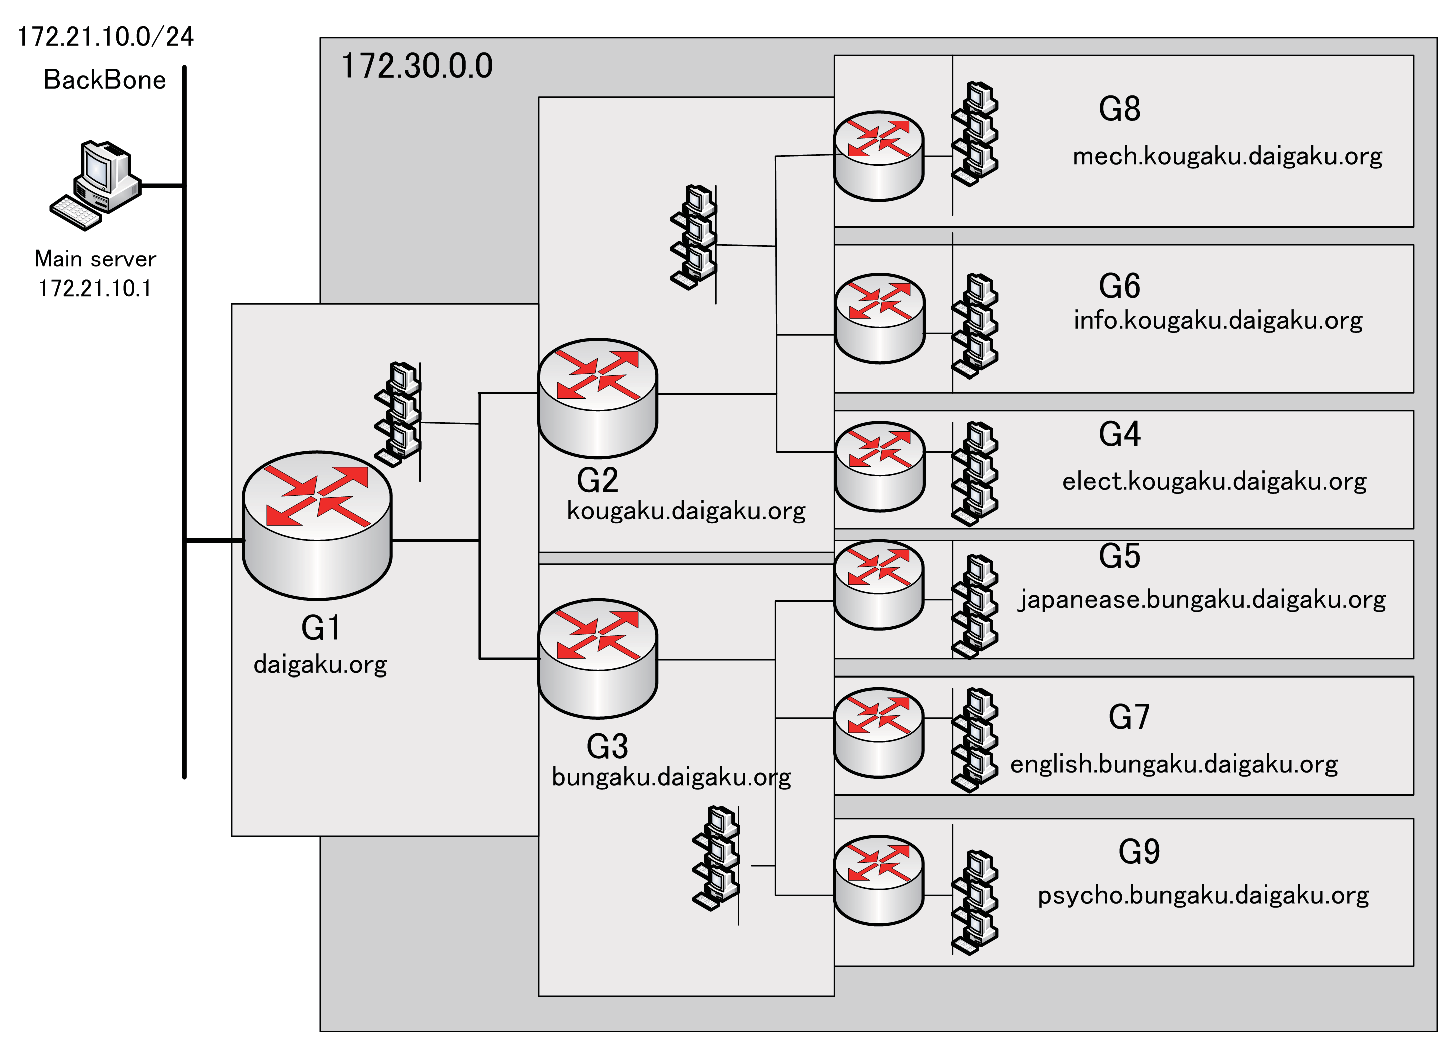
\includegraphics{./etc/specs/final.eps}}
\vspace*{-1zh}
\end{center}
\caption{最終課題構成図}
\label{final:fig:finalnet}
\end{figure}
ただし,ここで使用しているグループやドメインは仮のものであり,どのグルー
プがどこを担当し,どのようなドメイン・サブドメインにするかは後ほど決定
する.

\subsection{要求仕様}

\subsubsection{各グループのIPアドレスの割り当て}
G1以下の全体のネットワークに 172.30.0.0(ナチュラルマスク)のネットワー
クが割り当てられているので,各グループ同士で協議の上,サブネット化をし
て用いる.

\subsubsection{各グループの責任範囲}
各グループが責任を持って設定しなければならない範囲は,各グループのルー
タの上流側インターフェイスの接続・設定から下流側のサブネットワークの全
ての機器(スイッチングハブ,サーバ,コンピュータ,周辺機器,ケーブル)
である.ただし下流側ルータのインターフェイス接続は,下流側グループの担
当となる.

\subsubsection{各グループのルータのIPアドレス}
\begin{itemize}
\item 各サブネットの最も小さい IP アドレスから付与する.
\item サブネット内に複数のルータがある場合は,グループ番号の小さいものから順に付与する.
\end{itemize}

\subsubsection{ルーティング}
\begin{itemize}
\item 静的ルーティングを用いる.
\item 各ワークステーション,コンピュータ等は,デフォルトゲートウェイとして自
グループの上位側ルータを指定する.
\end{itemize}

\subsubsection{DNS ドメインの構成}
\begin{itemize}
\item G1 以下の全体ネットワークに daigaku.org ドメインが付与されている.
\item G1 が daigaku.org ゾーンを管理し,G2,G3 にそれぞれサブドメイン
  kougaku, bungaku を割り当てて,それらのゾーンを委譲する.
\item G2 は kougaku.daigaku.org ゾーンを管理し,G4,G6,G8 にそれぞれ
  elect,info,mech サブドメインを割り当て,ゾーンを委譲をする.
\item G3 は bungaku.daigaku.org ゾーンを管理し,G5,G7,G9 にそれぞれ
  japanese,english,psycho サブドメインを割り当て,ゾーンを委譲をする.
\item G4 は elect.kougaku.daigaku.org ゾーンを管理する.
\item G5 は japanese.bungaku.daigaku.org ゾーンを管理する.
\item G6 は info.kougaku.daigaku.org ゾーンを管理する.
\item G7 は english.bungaku.daigaku.org ゾーンを管理する.
\item G8 は mech.kougaku.daigaku.org ゾーンを管理する.
\item G9 は psycho.bungaku.daigaku.org ゾーンを管理する.
\item 逆引きは考えなくてよい(設定を行う必要はない).
\end{itemize}

\subsubsection{外部ネットワークとの接続}
\begin{itemize}
\item 各グループのサーバ間は,接続可能であること.
\item 各グループのサーバは,Mail server 172.21.10.1 に接続可能であること.
\item 各グループのサーバは,backbone 172.21.10.0/24 に接続可能であること.
\end{itemize}

\subsubsection{サービス}
\begin{itemize}
\item 全ての端末からメール送受信,ウェブ閲覧が行えること.
\item メールアカウントは全員分作成する.
\item その他,必要と感じるサービス,便利であると考えるサービスがあれば
  構築する.構築したサービスについては,レポートに記述すること.
\end{itemize}


\subsubsection*{考慮すべき点}
\begin{itemize}
\item どのようにネットワークの設計を行うか
\item どのような設定をして要求する仕様を満たすか.
\item ネットワークのポリシーはどのように設定すべきか.
\item 他者との共同作業をどのように行うべきか.
\item どこまでが自分の責任範囲で,どこからが他者に責任範囲か.
\item 他者への設定依頼はどのようにすべきか.
\end{itemize}


\clearpage


%------------------------------------------------------------------- 参考文献
%\input{reference.tex}

\end{document}
